\documentclass[letterpaper,12pt,twoside]{book}
\usepackage[spanish,es-noshorthands]{babel}

%%%%%%%%%%%%%%%%%%%%%%%%%%%%%%%%%%%%%%%%%%%%%%
%%%          Se incluye el preámbulo       %%%
%%%%%%%%%%%%%%%%%%%%%%%%%%%%%%%%%%%%%%%%%%%%%%
% ==================================================
% Fuentes, idioma y codificación
% ==================================================
\usepackage[T1]{fontenc}        % Acentos correctos en PDF
\usepackage[utf8]{inputenc}     % Archivos fuente en UTF-8
\usepackage[spanish]{babel}     % Español (títulos, fechas, etc.)
\decimalpoint                   % Usar punto decimal

% Fuente moderna (texto + mejor rasterizado)
\usepackage{lmodern}
%\usepackage{stix}

\usepackage[table]{xcolor} % Para pintar las celdas y filas
\usepackage{graphicx}      % Para el \resizebox
\usepackage{tikz}          % Para dibujar los cuadritos de la leyenda




% ==================================================
% Matemáticas
% ==================================================
\usepackage{amsmath, amssymb, mathtools}
% Opcionales de mates avanzadas (descomenta solo si los usas)
% \usepackage{physics}
%\usepackage{tensor}
% \usepackage{cancel}
\usepackage{empheq}             % Para enmarcar/destacar ecuaciones

% ==================================================
% Página, espaciado y párrafos
% ==================================================
\usepackage{setspace}

% ==================================================
% Cabeceras y pies de página
% ==================================================
%\usepackage{fancyhdr}
%\setlength{\headheight}{14.5pt}
%\pagestyle{fancy}


% ==================================================
% Tablas, múltiples columnas, etc.
% ==================================================
\usepackage{booktabs}           % Tablas bonitas
% \usepackage{multirow}         % Solo si usas celdas de varias filas
\usepackage{multicol}           % Texto en varias columnas

% ==================================================
% Colores, figuras y gráficos
% ==================================================
\usepackage{xcolor}
\usepackage{graphicx}
\graphicspath{{Figuras/}{logo/}}
\usepackage{float}
\usepackage{subcaption}
\usepackage{tikz}
\usetikzlibrary{positioning, shapes, matrix, fit, backgrounds, arrows.meta}
\pgfdeclarelayer{background}
\pgfdeclarelayer{foreground}
\pgfsetlayers{background,main,foreground}

\usepackage{pgfplots}
\pgfplotsset{
    width=10cm,
    compat=1.18    % versión moderna recomendada
}

% ==================================================
% Títulos de secciones (estética)
% ==================================================
\usepackage{titlesec}
\definecolor{gray75}{gray}{0.75}
\newcommand{\hsp}{\hspace{20pt}}

% Como extarticle/article NO tienen \chapter, formateamos \section:
\titleformat{\section}[hang]
  {\Large\bfseries}
  {\thesection\hsp\textcolor{gray75}{|}\hsp}
  {0pt}
  {\Large\bfseries}

% ==================================================
%  Descomentar para puntos en la tabla de contenidos
% ==================================================

%\usepackage{tocloft}
%\renewcommand{\cftsecleader}{\cftdotfill{\cftdotsep}}
%\sidecaptionvpos{figure}{tl}

% ==================================================
% Cajas de color / bloques (tcolorbox)
% ==================================================
%\usepackage{tcolorbox}
%\tcbuselibrary{skins,breakable}

% ==================================================
% Enlaces
% ==================================================
\usepackage[hidelinks]{hyperref}

%%%%%%%%%%%%%%%%%%%%%%%%%%%%%%%%%%%%%%%%%
%%%%%      Underline Eqs        %%%%%%%%%
%%%%%%%%%%%%%%%%%%%%%%%%%%%%%%%%%%%%%%%%%

\newsavebox\MBox
\newcommand\Cline[2][red]{{\sbox\MBox{$#2$}%
  \rlap{\usebox\MBox}\color{#1}\rule[-1.2\dp\MBox]{\wd\MBox}{0.5pt}}}
%%%%%%%%%%%%%%%%%%%%%%%%%%%%%%%%%%%%%%%%%%
%%%        CONSTANTES                %%%%%
%%%%%%%%%%%%%%%%%%%%%%%%%%%%%%%%%%%%%%%%%%
\newcommand\mom{\sqrt{\frac{m\omega}{2\hbar}}}
\newcommand\momsq{\frac{m\omega}{2\hbar}}
\newcommand\dad{\sqrt{\frac{m\omega\hbar}{2}}ie^{-\abs{z}^2/2}}
\newcommand\gus{\sqrt{\frac{\hbar}{2m\omega}}}
\newcommand\gussq{\frac{\hbar}{2m\omega}}
\newcommand\adag{\hat{a}^{\dagger}}
\newcommand\ah{\hat{a}}

\newcommand{\ylm}[2]{Y_{#1}^{#2}}
\newcommand{\fun}[3]{\Psi_{#1 #2 #3}(r,\theta,\phi)=R_{#1 #2}(r)Y_{#2}^{#3}(\theta,\phi)}
\newcommand{\funup}[3]{\Psi_{#1 #2 #3,\,+\frac{1}{2}}(r,\theta,\phi)=R_{#1 #2}(r)Y_{#2}^{#3}(\theta,\phi)}
\newcommand{\fundown}[3]{\Psi_{#1 #2 #3,\,-\frac{1}{2}}(r,\theta,\phi)=R_{#1 #2}(r)Y_{#2}^{#3}(\theta,\phi)}
%%%%%%%%%%%%%%%%%%%%%%%%%%%%%%%%%%%%%%%%%%%
%%%%     PALETA DE COLORES         %%%%%%%%
%%%%%%%%%%%%%%%%%%%%%%%%%%%%%%%%%%%%%%%%%%%
\definecolor{Verde}{HTML}{31B189}
\definecolor{Azul}{HTML}{7ACE67}
\definecolor{Naranja}{HTML}{FFC872}
% Paleta compartida con la presentación y el póster.
\definecolor{marinoCIMAT}{HTML}{0A1A2F}
\definecolor{vinoCIMAT}{HTML}{7A2237}
\definecolor{petroleo}{HTML}{3B5366}
\definecolor{fondoSlide}{HTML}{F4F5F7}
\definecolor{textoBody}{HTML}{1A1A1A}
\definecolor{textoSec}{HTML}{4A4A4A}
\definecolor{csvEconomico}{HTML}{A8C8E0}
\definecolor{csvComorbilidad}{HTML}{E89D9D}
\definecolor{csvTrabajoSocial}{HTML}{A8D5BA}
\definecolor{umapEconomico}{HTML}{378ADD}
\definecolor{umapComorbilidad}{HTML}{D85A30}
\definecolor{umapTrabajoSocial}{HTML}{1D9E75}
\definecolor{easyPositive}{HTML}{A8D5BA}
\definecolor{hardPositive}{HTML}{FFC966}
\definecolor{easyNegative}{HTML}{D8D8D8}
\definecolor{hardNegative}{HTML}{E89D9D}
\definecolor{bloqueCode}{HTML}{1C1C1E}
\definecolor{tokenCyan}{HTML}{5BD9C8}
\definecolor{tokenVerde}{HTML}{7EDFA5}
\definecolor{tokenVioleta}{HTML}{B4A3E8}
\definecolor{semVerde}{HTML}{4CAF50}
\definecolor{semAmarillo}{HTML}{FFC107}
\definecolor{semRojo}{HTML}{E53935}
\definecolor{Crema}{HTML}{FFE3B3}
\definecolor{AzulUV}{HTML}{1C36A1}
\definecolor{VerdeUV}{HTML}{00AA33}
\definecolor{RCimat}{HTML}{73243D}
\definecolor{GCimat}{HTML}{ACAAAB}


%%%%%%%%%%%%%%%%%%%%%%%%%%%%%%%%%%%%%%%%%%%%%%
%%%        Configuración bloques grises    %%%
%%%%%%%%%%%%%%%%%%%%%%%%%%%%%%%%%%%%%%%%%%%%%%
\usetikzlibrary{positioning, shapes}
\pgfdeclarelayer{background}
\pgfdeclarelayer{foreground}
\pgfsetlayers{background,main,foreground}
\usepackage{tcolorbox}
\tcbuselibrary{skins,breakable}
\newenvironment{myblock}[1]{%
    \tcolorbox[beamer,
    noparskip,breakable,
    colback=white,       % Fondo blanco
    colframe=black,      % Borde negro
    coltitle=black,      % Color del título en negro
    coltext=black,       % Texto negro
    sharp corners,       % Esquinas sin redondear
    boxrule=1pt,         % Grosor de las líneas del borde
    enhanced jigsaw,     % Mejora la estructura del cuadro
    before skip=10pt,    % Espacio antes del cuadro
    after skip=10pt]}    % Espacio después del cuadro
    {\endtcolorbox}


\newtcbox{\othermathbox}[1][]{nobeforeafter, tcbox raise base, enhanced, sharp corners, colback=white!10, colframe=AzulUV!30!black,drop fuzzy shadow, left=1em, top=1em, right=1em, bottom=1em}

% Syntax: \colorboxed[<color model>]{<color specification>}{<math formula>}
\newcommand*{\colorboxed}{}
\def\colorboxed#1#{%
  \colorboxedAux{#1}%
}
\newcommand*{\colorboxedAux}[3]{%
  % #1: optional argument for color model
  % #2: color specification
  % #3: formula
  \begingroup
    \colorlet{cb@saved}{.}%
    \color#1{#2}%
    \boxed{%
      \color{cb@saved}%
      #3%
    }%
  \endgroup
}
% ==================================================
\usepackage{csquotes}
\usepackage[backend=biber, style=numeric, sorting = none]{biblatex} % Estilo APA automático
\addbibresource{Bibliografia/referencias.bib} % Llama a tu archivo nuevo


%%%%%%%%%%%%%%%%%%%%%%%%%%%%%%%%%%%%%%%%%%%%%%
%%%       Paquete para portada CIMAT       %%%
%%%%%%%%%%%%%%%%%%%%%%%%%%%%%%%%%%%%%%%%%%%%%%
\usepackage{CIMATpreamble}
\setlength{\headheight}{30pt}

%%%%%%%%%%%%%%%%%%%%%%%%%%%%%%%%%%%%%%%%%%%%%%
%%%     Datos de la portada CIMAT          %%%
%%%%%%%%%%%%%%%%%%%%%%%%%%%%%%%%%%%%%%%%%%%%%%
\title{Aprendizaje métrico y modelos de lenguaje pre-entrenados para la resolución de entidades en bases de datos clínicas}
\author{Ing. Uziel Isaí Luján López}
\documentType{T E S I S}
\degree{Maestro en Cómputo Estadístico}
\supervisor{Dr. Víctor Hugo Muñiz Sánchez}
\supervisorSecond{Dr. Víctor Mireles Chávez}
\cityandyear{Monterrey, Nuevo León, \today}

\begin{document}

%%%%%%%%%%%%%%%%%%%%%%%%%%%%%%%%%%%%%%%%%%%%%%
%%%      Portada oficial CIMAT             %%%
%%%%%%%%%%%%%%%%%%%%%%%%%%%%%%%%%%%%%%%%%%%%%%
\maketitle

%%%%%%%%%%%%%%%%%%%%%%%%%%%%%%%%%%%%%%%%%%%%%%
%%%        Frontmatter                     %%%
%%%%%%%%%%%%%%%%%%%%%%%%%%%%%%%%%%%%%%%%%%%%%%
\frontmatter

% --- Dedicatoria ---
\chapter*{}
\begin{flushright}
  \emph{A mis padres, por todo.}
  \thispagestyle{empty}
\end{flushright}

% --- Resumen ---
\chapter*{Resumen}
\addcontentsline{toc}{chapter}{Resumen}

Esta tesis aborda el problema de ligado de registros en bases de datos clínicas, tomando como caso de estudio registros de pacientes COVID-19 del Instituto Nacional de Enfermedades Respiratorias (INER). La ausencia de identificadores únicos confiables y la alta variabilidad en la captura de los datos motivan el diseño e implementación de un sistema basado en arquitecturas neuronales profundas y modelos de lenguaje pre-entrenados.

El sistema propuesto opera en dos etapas: recuperación de candidatos y clasificación de pares de registros. Los registros tabulares se transforman en secuencias estructuradas de texto mediante su serialización en formato clave-valor. En la primera etapa, un Bi-Encoder, entrenado con la función de pérdida \textit{Multiple Negatives Ranking Loss} (MNRL), construye un espacio métrico compartido, proyecta los registros en él y recupera eficientemente los candidatos con mayor similitud semántica. En la segunda etapa, cada registro de consulta se empareja con cada uno de los candidatos recuperados. Un Cross-Encoder, entrenado con \textit{Binary Cross Entropy} (BCE), procesa conjuntamente los dos registros para clasificarlos o no como la misma entidad.

También se exploran estrategias de aumento de datos diseñadas para mitigar la desproporción entre pares positivos y negativos y favorecer la capacidad de generalización de los modelos. Los experimentos no evidenciaron una mejora en dicha capacidad, debido a que los patrones sintéticos implementados no reprodujeron adecuadamente la variabilidad de los datos reales.

En conjunto, los resultados muestran que la propuesta logra un equilibrio entre eficiencia y precisión sobre el conjunto de datos construido a partir de los registros clínicos del INER, lo que respalda su integración como un sistema confiable para el ligado de registros clínicos heterogéneos con información faltante.


\paragraph{Palabras clave:} aprendizaje métrico, resolución de entidades, modelos de lenguaje, ligado de registros, registros clínicos

% --- Agradecimientos ---
\chapter*{Agradecimientos}
\addcontentsline{toc}{chapter}{Agradecimientos}

Texto de agradecimientos.

% --- Tabla de contenidos y listas ---
\tableofcontents
\clearpage

\listoffigures
\clearpage

%%%%%%%%%%%%%%%%%%%%%%%%%%%%%%%%%%%%%%%%%%%%%%
%%%        Mainmatter                      %%%
%%%%%%%%%%%%%%%%%%%%%%%%%%%%%%%%%%%%%%%%%%%%%%
\mainmatter

\spacing{1.5}

%%%%%%%%%%%%%%%%%%%%%%%%%%%%%%%%%%%%%%%%%%%%%%
%%%       Capítulos de la Tesis            %%%
%%%%%%%%%%%%%%%%%%%%%%%%%%%%%%%%%%%%%%%%%%%%%%
\chapter{Introducción}

\section{Contexto y motivación}
La integración de información proveniente de múltiples fuentes es un problema central en el análisis de datos dentro de instituciones públicas. Particularmente en el contexto del sector salud, las bases de datos suelen ser inherentemente heterogéneas, con estructuras dispares, catálogos incompletos, errores de captura, duplicidades y un alto grado de información faltante~\cite{cappuzzo2020,ong2014}. Estas condiciones dificultan enormemente la vinculación de registros que se refieren a la misma entidad o persona, lo cual limita la capacidad de las instituciones para generar diagnósticos confiables y tomar decisiones informadas.

El Instituto Nacional de Enfermedades Respiratorias Ismael Cosío Villegas (INER) experimentó una exacerbación de este fenómeno durante la emergencia sanitaria por COVID-19. La necesidad operativa de atender volúmenes masivos de pacientes obligó a la captura acelerada de información a través de múltiples sistemas independientes entre sí (administrativos, clínicos y de trabajo social). Consolidar estas fuentes fragmentadas no es solo un requerimiento para la optimización administrativa, sino un paso clínico fundamental: garantizar que la calidad, interoperabilidad y consistencia de los registros permitan un seguimiento riguroso y unificado para los pacientes post-COVID-19. La posibilidad de construir herramientas que identifiquen coincidencias de manera precisa, transparente y escalable tiene un impacto potencial directo en la operación institucional del INER.

\section{Planteamiento del problema}
El desafío central para la integración de las bases de datos del INER radica en la ausencia de identificadores únicos estandarizados. Aunque dentro de dichas bases  existan campos teóricamente vinculantes, como el número de expediente o el nombre del paciente, estos fungen como llaves ``rotas'' debido a la naturaleza ruidosa de la captura humana en el mundo real, sobre todo en situaciones de emergencia sanitaria.

Al proceso de identificar registros coincidentes entre bases de datos distintas se le conoce en la literatura como Ligado de Registros (\textit{Record Linkage}) o Resolución de Entidades~\cite{dunn1946,fellegi1969,li2020} y es fundamental para obtener una visión coherente y completa de la información disponible. Los métodos clásicos para abordar este problema, basados en reglas condicionales rígidas o comparaciones de cadenas de caracteres (como distancias de edición~\cite{levenshtein1966,damerau1964} o métricas de similitud de cadenas~\cite{jaro1989}), ofrecen soluciones aceptables únicamente cuando los datos son consistentes y relativamente limpios. Sin embargo, resultan insuficientes ante la variabilidad lingüística, la presencia de errores ortográficos y tipográficos o la existencia de texto libre con ambigüedad semántica~\cite{li2020}.
Estas limitaciones se vuelven particularmente críticas en dominios sensibles como la atención médica, donde un error de vinculación puede afectar directamente la calidad de vida de una persona o el seguimiento clínico de un caso específico.

En años recientes, los avances en técnicas de aprendizaje profundo y procesamiento de lenguaje natural han abierto nuevas posibilidades para abordar este problema. Los modelos de lenguaje pre-entrenados basados en la arquitectura Transformer~\cite{vaswani2017}, como BERT~\cite{devlin2019}, han demostrado una alta capacidad para capturar relaciones semánticas y desambiguar texto en contextos complejos, permitiendo modelar distancias robustas entre registros heterogéneos. Estas herramientas son especialmente útiles cuando se requiere comparar información almacenada en formatos distintos~\cite{li2020,cappuzzo2020} (e.g. comparar texto libre con datos tabulares) y trabajar con información incompleta o ruidosa~\cite{ong2014,li2020}.

Sin embargo, a este desafío de calidad y heterogeneidad presentes en los datos se suma una barrera computacional crítica: la comparación y revisión exhaustiva de todos los pares posibles en bases de datos masivas conlleva una complejidad cuadrática $\mathcal{O}(N^2)$. Aplicar directamente a esta escala arquitecturas neuronales profundas, como los Transformers, resulta prohibitivo debido a su alto costo computacional.

Por lo tanto, existe una necesidad relevante de superar tanto las limitaciones léxicas como los cuellos de botella computacionales. Se requiere un sistema moderno capaz de comprender e integrar el contexto semántico de la información del paciente, tolerar el ruido inherente a la captura humana, reducir drásticamente el espacio de búsqueda y estimar de manera efectiva si dos registros distintos corresponden a la misma entidad. Este escenario es de alta pertinencia en el contexto mexicano, donde la construcción de este tipo de herramientas tiene un impacto directo tanto en la operación institucional como en el bienestar de la población.


\section{Objetivos}

\subsection{Objetivo general}
Diseñar e implementar un sistema robusto para el ligado de registros entre bases de datos heterogéneas, basado en una arquitectura neuronal profunda de dos etapas: recuperación de candidatos y clasificación de pares de registros.

Evaluar y validar el sistema mediante la vinculación de registros clínicos proporcionados por el Instituto Nacional de Enfermedades Respiratorias (INER), estableciendo una estructura modular y una metodología reproducible para la integración de información en el sector público de salud.

\subsection{Objetivos específicos}

\begin{enumerate}
    \item Definir bloques semánticos que permitan organizar adecuadamente los atributos de las bases de datos del INER de acuerdo con las modalidades de información que representan.
    \item Construir representaciones textuales estructuradas de los registros mediante la serialización y concatenación de sus bloques semánticos en una única secuencia con formato clave-valor, definido a partir de la inclusión de tokens especiales.
    \item Implementar una etapa de recuperación entrenando un modelo basado en una arquitectura neuronal de tipo siamesa (Bi-Encoder), que construya un espacio métrico compartido y sea capaz de proyectar los registros en él, permitiendo recuperar los registros candidatos a ser la misma entidad.
    \item Desarrollar una fase de clasificación entrenando un modelo basado en una arquitectura que emplee el mecanismo de autoatención (Cross-Encoder) como clasificador binario de los pares formados a partir de los registros recuperados en la etapa anterior, con el propósito de estimar si corresponden a la misma entidad.
    \item Analizar el efecto de estrategias de aumento de datos sobre la desproporción entre pares positivos y negativos y la capacidad de generalización de los modelos ante el ruido y la variabilidad presentes en registros no observados durante el entrenamiento.
    \item  Evaluar el desempeño de las etapas de recuperación y clasificación, así como el comportamiento integral del sistema, mediante métricas apropiadas para cada componente.
\end{enumerate}


\section{Contribución de la tesis}

La principal aportación de este trabajo de tesis reside en el diseño metodológico y la implementación de un sistema robusto y moderno que vincula la ingeniería de datos con el aprendizaje profundo aplicado al sector salud. Mientras que las soluciones convencionales dependen de procesos de limpieza manual y revisión exhaustiva, así como de reglas condicionales frágiles ante el error humano, esta tesis demuestra que los modelos de lenguaje pre-entrenados pueden tolerar y absorber el ruido inherente a los datos del mundo real si se les proporciona la estructura y el contexto adecuados.

Al evolucionar de métricas de similitud léxica clásicas hacia una arquitectura neuronal profunda de dos etapas, el sistema propuesto aborda el compromiso entre eficiencia y precisión. La etapa de recuperación reduce el espacio de búsqueda evitando la necesidad de analizar todos los posibles pares mediante la selección de registros candidatos, mientras que la etapa de clasificación analiza en detalle los pares formados a partir de estos candidatos para determinar si efectivamente corresponden a la misma entidad.

Adicionalmente, se analiza una estrategia de aumento de datos diseñada para mitigar la desproporción entre pares positivos y negativos y favorecer la capacidad de generalización de los modelos. Aunque los experimentos no evidenciaron una mejora en dicha capacidad, permitieron identificar las limitaciones del mecanismo sintético implementado para reproducir los patrones de variabilidad presentes en los datos reales. En conjunto, el proyecto proporciona una estructura modular y una metodología reproducible que pueden servir como base para desarrollar herramientas de integración de información en instituciones públicas que carecen de identificadores únicos confiables.

\chapter{Marco teórico y estado del arte}

% 2.1 EL PROBLEMA MATEMÁTICO

\section{El problema de ligado de registros (\textit{Record Linkage})}

El ligado de registros (\textit{Record Linkage}) constituye un problema fundamental para la integración de información proveniente de fuentes de datos heterogéneas y fragmentadas. En la literatura de ciencias de la computación, particularmente en las áreas de bases de datos e integración de información, este problema se relaciona estrechamente con la resolución o emparejamiento de entidades (\textit{Entity Resolution} o \textit{Entity Matching})~\cite{li2020,cappuzzo2020}. En ambos casos, el objetivo es determinar si dos o más registros provenientes de distintas fuentes representan a la misma entidad del mundo real, especialmente cuando no existe un identificador único global y confiable. La complejidad del problema se incrementa ante la presencia de errores tipográficos, variaciones en la grafía, campos faltantes y diferencias en los formatos de almacenamiento, lo que convierte su resolución en un desafío estadístico y computacional relevante.

Desde una perspectiva histórica, el concepto fue introducido formalmente por Dunn~\cite{dunn1946} en 1946, quien visualizó el ligado de registros como una herramienta esencial para la creación de un sistema de información longitudinal que permitiera el seguimiento de individuos a lo largo de su ciclo de vida. No obstante, la formalización matemática y probabilística del problema no se consolidaría sino hasta 1969, con el trabajo seminal de Fellegi y Sunter~\cite{fellegi1969}. Su modelo establece un marco de decisión basado en la teoría de pruebas de hipótesis, donde cada par de registros es clasificado en una de tres categorías: enlace (\textit{link}), no enlace (\textit{non-link}) o caso indeciso (\textit{clerical review}), basándose en la probabilidad de observar ciertas concordancias en los atributos dado que el par es realmente un duplicado o no.

Matemáticamente, sean $A$ y $B$ dos conjuntos de registros, con $n=|A|$ y $m=|B|$, y sea $e(r)$ la entidad del mundo real representada por un registro $r$. El conjunto de enlaces verdaderos puede expresarse como la relación

\[
M=\{(a,b)\in A\times B : e(a)=e(b)\}.
\]

El objetivo del ligado de registros es estimar $M$ a partir de los atributos observados, dado que la identidad representada por cada registro no se conoce de manera directa. Una estrategia exhaustiva requiere evaluar los $n\cdot m$ pares contenidos en el producto cartesiano $A\times B$, por lo que su complejidad es $\mathcal{O}(nm)$. Cuando ambas bases tienen tamaños comparables, es decir, $n\approx m\approx N$, esta complejidad puede expresarse como $\mathcal{O}(N^2)$. En contextos institucionales como el del INER, este crecimiento representa una barrera computacional que exige mecanismos eficientes para reducir el espacio de candidatos.

En la literatura contemporánea, la resolución de entidades se utiliza como un concepto amplio que abarca tareas relacionadas, como el ligado de registros entre distintas fuentes y la deduplicación dentro de una misma base de datos~\cite{christen2012}. En esta tesis, el problema se aborda desde una perspectiva semántica, con el objetivo de superar las limitaciones de la comparación sintáctica mediante representaciones vectoriales aprendidas.

% 2.2 ENFOQUES CLÁSICOS Y MÉTRICAS DE SIMILITUD LÉXICA
%
\section{Enfoques clásicos y métricas de similitud léxica}

Históricamente, el tratamiento del ligado de registros ha dependido de la comparación sintáctica de cadenas de caracteres (\textit{strings}). Estos métodos, se dividen principalmente en métricas basadas en edición, comparadores de caracteres y métodos basados en tokens. Su objetivo es cuantificar la discrepancia entre dos cadenas para decidir si representan un mismo valor.

\subsection{Métricas basadas en edición y comparadores}

\paragraph{Distancia de Levenshtein.}
La distancia de Levenshtein~\cite{levenshtein1966} cuantifica la diferencia entre dos cadenas como el número mínimo de inserciones, eliminaciones o sustituciones de caracteres necesarias para transformar una en la otra. Para expresar el resultado como una similitud en el intervalo $[0,1]$, la distancia puede dividirse entre la longitud de la cadena más larga y restarse de 1; de este modo, una similitud de 1 indica una coincidencia exacta.

Una variante relevante es la distancia de Damerau-Levenshtein~\cite{damerau1964}, que incorpora la transposición de caracteres adyacentes como una operación elemental. La Tabla~\ref{tab:ejemplo_distancias_edicion} muestra la diferencia entre ambas métricas ante un error común de mecanografía.

\begin{table}[H]
\centering
\caption{Ejemplo de las distancias de Levenshtein y Damerau-Levenshtein}
\label{tab:ejemplo_distancias_edicion}
\small
\begin{tabular}{>{\raggedright\arraybackslash}p{2.6cm}
                >{\raggedright\arraybackslash}p{2.5cm}
                >{\raggedright\arraybackslash}p{4.5cm}
                >{\raggedright\arraybackslash}p{3.8cm}}
\toprule
\textbf{Métrica} & \textbf{Cadenas} & \textbf{Interpretación} & \textbf{Cálculo} \\
\midrule
Levenshtein
  & \texttt{MARIA} $\rightarrow$ \texttt{MAIRA}
  & Requiere sustituir \texttt{R} por \texttt{I} y \texttt{I} por \texttt{R}. Dos operaciones de edición.
  & Distancia: $d=2$

    \vspace{2pt}
    $\operatorname{sim}=1-\dfrac{2}{5}$

    \vspace{2pt}
    $\operatorname{sim}=0.60$ \\
\addlinespace
Damerau-Levenshtein
  & \texttt{MARIA} $\rightarrow$ \texttt{MAIRA}
  & Reconoce el intercambio \texttt{RI} $\rightarrow$ \texttt{IR} como una sola transposición.
  & Distancia: $d=1$

    \vspace{2pt}
    $\operatorname{sim}=1-\dfrac{1}{5}$

    \vspace{2pt}
    $\operatorname{sim}=0.80$ \\
\bottomrule
\end{tabular}
\end{table}

\paragraph{Índice de Jaro y Jaro-Winkler.}
El índice de Jaro~\cite{jaro1989} mide la similitud entre dos cadenas considerando la cantidad de caracteres coincidentes, su posición relativa y las transposiciones necesarias para alinearlos. Su valor pertenece al intervalo $[0,1]$, donde 1 indica una coincidencia exacta. Jaro-Winkler~\cite{winkler1990} extiende esta medida y otorga mayor peso a las cadenas que comparten los primeros caracteres, una propiedad útil para comparar nombres propios.

La Tabla~\ref{tab:ejemplo_jaro_winkler} ilustra el efecto de esta corrección. Las cadenas \texttt{MARTHA} y \texttt{MARHTA} contienen los mismos caracteres, pero presentan una transposición. Jaro les asigna una similitud alta y Jaro-Winkler la incrementa porque ambas comienzan con el prefijo \texttt{MAR}.

\begin{table}[H]
\centering
\caption{Ejemplo de los índices de Jaro y Jaro-Winkler (MARTHA VS MARHTA)}
\label{tab:ejemplo_jaro_winkler}
\small
\begin{tabular}{>{\raggedright\arraybackslash}p{2.7cm}
                >{\raggedright\arraybackslash}p{5.6cm}
                >{\raggedright\arraybackslash}p{5.0cm}}
\toprule
\textbf{Índice} & \textbf{Información considerada} & \textbf{Cálculo} \\
\midrule
Jaro
  & Coincidencia de caracteres y transposición entre \texttt{TH} y \texttt{HT}.
  & Coincidencias: $m=6$

    Transposiciones: $t=1$

    \vspace{2pt}
    $J=\dfrac{1}{3}\left(1+1+\dfrac{5}{6}\right)$

    \vspace{2pt}
    $J=\dfrac{17}{18}\approx0.944$ \\
\addlinespace
Jaro-Winkler
  & Puntuación de Jaro más el peso adicional por el prefijo compartido \texttt{MAR}.
  & Longitud del prefijo: $\ell=3$

    Factor de escala: $p=0.1$

    \vspace{2pt}
    $JW=0.944+3(0.1)(1-0.944)$

    \vspace{2pt}
    $JW\approx0.961$ \\
\bottomrule
\end{tabular}
\end{table}

\paragraph{Métodos basados en $q$-gramas.}
Por otro lado, enfoques basados en fragmentos de texto o $q$-gramas~\cite{ukkonen1992} permiten una comparación más flexible al descomponer las cadenas en sub-secuencias de longitud fija, facilitando la identificación de coincidencias parciales incluso cuando la edición acumulada es alta.

\subsection{Modelos probabilísticos y pesos de importancia}
Más allá de la comparación de una sola cadena, el modelo de Fellegi-Sunter~\cite{fellegi1969} proporcionó la base teórica para combinar múltiples comparaciones de atributos. En este modelo, cada atributo recibe un peso basado en su capacidad de discriminación; por ejemplo, una coincidencia en un apellido poco común tiene un peso mayor que una coincidencia en un nombre frecuente. En contextos textuales, también pueden emplearse técnicas de ponderación de términos como TF-IDF (\textit{Term Frequency-Inverse Document Frequency})~\cite{salton1988}, que permiten identificar qué palabras dentro de un registro son más informativas para el proceso de vinculación.

\subsection{Limitaciones de la comparación sintáctica}
Las métricas sintácticas descritas anteriormente resultan útiles cuando las diferencias entre los registros se limitan a variaciones superficiales en su escritura. Sin embargo, sus comparaciones se derivan principalmente de la coincidencia de caracteres o tokens y no representan explícitamente el significado ni el contexto de la información~\cite{christen2012,barlaug2021}. En consecuencia, dos valores con formas léxicas distintas pueden recibir una similitud baja aun cuando sean semánticamente equivalentes; de manera inversa, dos cadenas similares pueden corresponder a entidades diferentes. En las bases de datos clínicas, la variación terminológica, las abreviaturas y la presencia de texto libre acentúan esta limitación. Esta brecha motiva la transición hacia representaciones vectoriales aprendidas y modelos neuronales para el emparejamiento de entidades~\cite{barlaug2021,li2020}.

% 2.3 EL CAMBIO DE PARADIGMA: APRENDIZAJE PROFUNDO Y MODELOS DE LENGUAJE PRE-ENTRENADOS

\section{Aprendizaje profundo y modelos de lenguaje pre-entrenados}

Los avances recientes en los enfoques neuronales para la resolución de entidades se han beneficiado de la evolución de las representaciones vectoriales en el procesamiento de lenguaje natural (PLN)~\cite{barlaug2021}. A diferencia de las métricas léxicas descritas anteriormente, los \textit{embeddings} densos codifican patrones distribucionales en espacios continuos, lo que permite aprovechar similitudes que no se reducen a coincidencias exactas de caracteres o tokens~\cite{li2020}. Sin embargo, las ventajas del aprendizaje profundo no son uniformes para todos los tipos de datos: el estudio sistemático de Mudgal et al.~\cite{mudgal2018} encontró sus principales beneficios en problemas de emparejamiento con registros textuales o ruidosos, mientras que en datos estructurados y limpios los métodos convencionales podían conservar un desempeño competitivo.

\subsection{De representaciones dispersas a vectores densos}
Las representaciones tradicionales del texto, como los vectores de conteos y TF-IDF, asignan dimensiones independientes a los términos del vocabulario, lo que produce vectores dispersos de alta dimensionalidad~\cite{salton1988}. Aunque estas representaciones permiten cuantificar la importancia y coincidencia de los términos, no construyen por sí mismas un espacio continuo en el que palabras relacionadas ocupen posiciones cercanas.

Uno de los antecedentes fundamentales del modelado semántico mediante redes neuronales es el modelo de lenguaje probabilístico propuesto por Bengio et al.~\cite{bengio2003}, que permitió aprender representaciones distribuidas de palabras conjuntamente con la función de probabilidad de secuencias textuales.

\paragraph{Representaciones estáticas.}
Este paradigma se consolidó con Word2Vec~\cite{mikolov2013}, que aprende vectores a partir de los contextos locales en los que aparecen las palabras, y con GloVe~\cite{pennington2014}, que incorpora estadísticas globales de coocurrencia del corpus. En ambos casos, las regularidades lingüísticas se representan mediante relaciones geométricas en un espacio continuo.

FastText~\cite{bojanowski2017} extendió este enfoque al representar cada palabra a partir de unidades subléxicas o $n$-gramas de caracteres. Esta composición permite obtener representaciones para palabras poco frecuentes o no observadas durante el entrenamiento y aprovechar regularidades morfológicas, lo que resulta útil en vocabularios amplios y especializados.

\paragraph{Representaciones contextualizadas mediante redes recurrentes.}
A pesar de sus diferencias, Word2Vec, GloVe y FastText producen representaciones estáticas: una palabra recibe el mismo vector independientemente del contexto en que aparezca. Así, el término ``alta'' tendría una única representación aunque pudiera referirse al egreso hospitalario o describir una magnitud elevada.

Los modelos contextuales abordaron esta limitación al calcular la representación de cada palabra en función de la secuencia completa. ELMo~\cite{peters2018}, basado en un modelo de lenguaje bidireccional con redes LSTM, genera vectores que cambian según el contexto y permiten modelar fenómenos como la polisemia. Esta distinción entre representaciones estáticas y contextualizadas proporciona el antecedente conceptual para las arquitecturas basadas en atención descritas en la subsección siguiente.

\subsection{La arquitectura Transformer y el mecanismo de atención}
La arquitectura Transformer, propuesta por Vaswani et al.~\cite{vaswani2017}, estableció un modelo de procesamiento de secuencias basado exclusivamente en mecanismos de atención, prescindiendo de estructuras recurrentes y convolucionales. Una de sus operaciones centrales es la atención de producto punto escalado (\textit{Scaled Dot-Product Attention}). En el caso de la autoatención, las representaciones de una misma secuencia se proyectan linealmente en tres matrices: consultas ($Q$), claves ($K$) y valores ($V$). La salida se calcula como una suma ponderada de los valores, donde los pesos reflejan la compatibilidad entre cada consulta y las claves:

\begin{equation}
\text{Attention}(Q, K, V) = \text{softmax}\!\left(\frac{Q K^\top}{\sqrt{d_k}}\right) V
\label{eq:scaled_dot_product_attention}
\end{equation}

donde $d_k$ es la dimensionalidad de las claves. El factor $\sqrt{d_k}$ evita que los productos punto alcancen magnitudes que saturen la función \textit{softmax} y produzcan gradientes demasiado pequeños. Esta operación permite calcular representaciones contextuales al ponderar la relevancia de cada token respecto de los demás elementos de la secuencia.

El Transformer emplea además atención multicabeza (\textit{Multi-Head Attention}), que ejecuta varias operaciones de atención en paralelo sobre proyecciones lineales distintas de $Q$, $K$ y $V$, y concatena sus resultados:

\begin{equation}
\text{MultiHead}(Q, K, V) = \text{Concat}(\text{head}_1, \dots, \text{head}_h) W^O
\label{eq:multihead}
\end{equation}

donde $\text{head}_i = \text{Attention}(Q W_i^Q, K W_i^K, V W_i^V)$. En registros tabulares serializados, este mecanismo permite que los tokens asociados con distintos atributos y valores intercambien información dentro de una representación contextual conjunta~\cite{li2020}.

\subsection{Modelos de lenguaje pre-entrenados (PLMs)}
La aplicación de Transformers a tareas de procesamiento de lenguaje natural se fortaleció mediante el preentrenamiento sobre corpus textuales de gran escala. Modelos como BERT (\textit{Bidirectional Encoder Representations from Transformers})~\cite{devlin2019} aprenden representaciones bidireccionales mediante objetivos autosupervisados y posteriormente pueden adaptarse a tareas específicas mediante ajuste fino (\textit{fine-tuning}). RoBERTa~\cite{liu2019} mostró que modificaciones en los datos, los hiperparámetros y el procedimiento de preentrenamiento podían mejorar el desempeño de este paradigma.

En esta tesis, los modelos preentrenados proporcionan el punto de partida para procesar las representaciones textuales de los registros del INER. El ajuste posterior adapta estos modelos a las dos tareas del sistema: construir un espacio métrico para la recuperación de candidatos y clasificar los pares de registros formados a partir de ellos.


% 2.4 ESTADO DEL ARTE EN LIGADO DE REGISTROS NEURONAL (SBERT Y DITTO)

\section{Estado del arte en ligado de registros}

La aplicación directa de modelos de lenguaje densos para evaluar el producto cartesiano de dos bases de datos masivas resulta computacionalmente prohibitiva. El paso de inferencia (\textit{Forward Pass}) de un Transformer basado en atención cruzada exhaustiva posee una complejidad cuadrática respecto a la longitud de la secuencia, lo que hace inviable calcular la similitud de millones de pares. Para mitigar este cuello de botella computacional, el estado del arte ha convergido hacia el paradigma \textit{Retrieve \& Re-rank} (Recuperación y Re-ordenamiento), una arquitectura de dos fases que equilibra eficiencia y precisión semántica.

\subsection{Aprendizaje métrico y recuperación eficiente con Bi-Encoders}

\paragraph{Aprendizaje métrico.}
El aprendizaje métrico busca construir un espacio de representación en el que la proximidad entre dos objetos refleje una relación relevante para la tarea~\cite{kulis2013}. En el ligado de registros, esta relación corresponde a la pertenencia a una misma entidad. Sea $\sigma$ la función que transforma un registro en una secuencia textual serializada y sea $\mathcal{X}$ el conjunto de secuencias que pueden utilizarse como entrada del modelo. Para dos registros $a\in A$ y $b\in B$, se define

\[
x_a=\sigma(a),
\qquad
x_b=\sigma(b).
\]

El codificador neuronal es una función parametrizada

\[
f_\theta:\mathcal{X}\longrightarrow\mathbb{R}^{d},
\]

que proyecta cada secuencia en un vector de dimensión fija. En consecuencia,

\[
\mathbf{z}_a=f_\theta(x_a),
\qquad
\mathbf{z}_b=f_\theta(x_b).
\]

La función $f_\theta$ no constituye por sí misma el espacio de representación; este corresponde a su imagen

\[
\mathcal{Z}_\theta
=f_\theta(\mathcal{X})
\subseteq\mathbb{R}^{d},
\]

cuya geometría depende de los parámetros aprendidos $\theta$. Cada elemento de $\mathcal{Z}_\theta$ es, por tanto, un \textit{embedding} a nivel de registro: una representación vectorial densa y aprendida que sintetiza la información contextual capturada por el Transformer a partir de la secuencia serializada. A diferencia de las representaciones estáticas de palabras descritas previamente, estos vectores representan registros completos y dependen tanto de su contenido como de la estructura proporcionada durante la serialización. De este modo, $\mathbf{z}_a$ y $\mathbf{z}_b$ son representaciones densas de $a$ y $b$, respectivamente, y sus relaciones geométricas codifican la similitud relevante para la tarea de ligado.

Al dotar $\mathcal{Z}_\theta$ con una función de similitud $\operatorname{sim}( \cdot)$, la similitud entre dos entradas puede escribirse como

\[
\operatorname{sim}_\theta(x_a,x_b)
=\operatorname{sim}\!\left(f_\theta(x_a),f_\theta(x_b)\right)
=\operatorname{sim}(\mathbf{z}_a,\mathbf{z}_b).
\]

El entrenamiento procura que dos registros de la misma entidad tengan una similitud alta en este espacio, mientras que los registros de entidades diferentes ocupen posiciones más alejadas:

\[
e(a)=e(b)\Rightarrow
\operatorname{sim}_\theta(x_a,x_b)\ \text{alta},
\qquad
e(a)\neq e(b)\Rightarrow
\operatorname{sim}_\theta(x_a,x_b)\ \text{baja}.
\]

En este enfoque no necesariamente se aprende una función de distancia nueva. En particular, el sistema puede utilizar una medida fija, como la similitud coseno, mientras aprende $f_\theta$ para organizar los registros dentro del espacio de representación. La estrategia de optimización empleada para obtener esta organización se describe posteriormente en la subsección dedicada al aprendizaje contrastivo.

\paragraph{Bi-Encoders y redes siamesas.}
Una red siamesa está formada por dos ramas que comparten arquitectura y parámetros, de modo que ambas aplican la misma función de codificación a entradas diferentes~\cite{bromley1993}. El término Bi-Encoder indica que los dos elementos de una comparación se codifican de forma independiente; cuando ambas ramas comparten sus parámetros, como en este trabajo, el Bi-Encoder constituye además una arquitectura siamesa.

Sentence-BERT (SBERT), propuesto por Reimers y Gurevych~\cite{reimers2019}, adapta modelos preentrenados como BERT a esta configuración. Cada secuencia se procesa por separado y las representaciones de sus tokens se agregan mediante una operación de \textit{pooling} para obtener un vector de dimensión fija. Formalmente, el codificador puede expresarse como $f_\theta=p\circ T_\theta$, donde $T_\theta$ es el Transformer que produce representaciones contextualizadas de los tokens y $p$ es la operación de \textit{pooling}. El mismo codificador se aplica de manera independiente a $x_a$ y $x_b$; sus tokens no interactúan directamente durante esta codificación. La comparación ocurre únicamente después de obtener $\mathbf{z}_a$ y $\mathbf{z}_b$, lo que permite calcular y almacenar cada representación una sola vez.

Reimers y Gurevych evaluaron tres estrategias de agregación: la media de las representaciones de salida (MEAN), su máximo por dimensión (MAX) y la representación asociada con el token \texttt{[CLS]}. MEAN fue su configuración predeterminada y obtuvo el mejor desempeño en la ablación presentada, aunque su ventaja fue reducida bajo el objetivo de clasificación y más clara bajo el objetivo de regresión semántica~\cite{reimers2019}. Por esta razón, en este trabajo $p$ corresponde a una operación de \textit{mean pooling}.

% Diagrama conceptual de un Bi-Encoder siamés para recuperación.
\providecolor{petroleo}{HTML}{3B5366}
\providecolor{vinoCIMAT}{HTML}{7A2237}
\begin{center}
\begin{tikzpicture}[
  >={Stealth[length=2.4mm]},
  flow/.style={->, draw=gray!65, line width=0.8pt},
  shared/.style={<->, draw=vinoCIMAT!70, dashed, line width=0.8pt},
  record/.style={draw=gray!45, fill=gray!6, rounded corners=3pt,
                 minimum width=2.1cm, minimum height=0.85cm, align=center},
  encoder/.style={draw=petroleo, fill=petroleo!10, rounded corners=3pt,
                  minimum width=2.2cm, minimum height=0.9cm, align=center},
  pooling/.style={draw=gray!45, fill=gray!8, rounded corners=3pt,
                  minimum width=1.7cm, minimum height=0.7cm, align=center},
  vector/.style={draw=petroleo, fill=white, circle, minimum size=0.8cm},
  similarity/.style={draw=vinoCIMAT, fill=vinoCIMAT!8, rounded corners=3pt,
                     minimum width=2.6cm, minimum height=0.9cm, align=center},
  every node/.style={font=\footnotesize}
]
  \node[record]  (recordA) at (-2.6,6.5) {Registro $x_a$};
  \node[record]  (recordB) at ( 2.6,6.5) {Registro $x_b$};
  \node[encoder] (encoderA) at (-2.6,4.9) {Codificador\\$f_\theta$};
  \node[encoder] (encoderB) at ( 2.6,4.9) {Codificador\\$f_\theta$};
  \node[pooling] (poolingA) at (-2.6,3.3) {\textit{mean pooling}};
  \node[pooling] (poolingB) at ( 2.6,3.3) {\textit{mean pooling}};
  \node[vector]  (vectorA) at (-2.6,1.75) {$\mathbf z_a$};
  \node[vector]  (vectorB) at ( 2.6,1.75) {$\mathbf z_b$};
  \node[similarity] (cosine) at (0,0.25) {Cálculo de\\similitud coseno};
  \node[draw=petroleo, fill=petroleo!8, rounded corners=3pt,
        minimum width=3.2cm, minimum height=0.75cm]
    (score) at (0,-1.25) {$\operatorname{sim}_\theta(x_a,x_b)$};

  \draw[flow] (recordA) -- (encoderA);
  \draw[flow] (recordB) -- (encoderB);
  \draw[flow] (encoderA) -- (poolingA);
  \draw[flow] (encoderB) -- (poolingB);
  \draw[flow] (poolingA) -- (vectorA);
  \draw[flow] (poolingB) -- (vectorB);
  \draw[flow] (vectorA) -- (cosine.north west);
  \draw[flow] (vectorB) -- (cosine.north east);
  \draw[flow] (cosine) -- node[right] {puntaje} (score);

  \draw[shared] (encoderA.east) -- (encoderB.west);
  \node[color=vinoCIMAT] at (0,5.25) {pesos compartidos};
\end{tikzpicture}
\captionof{figure}{Bi-Encoder siamés para aprendizaje métrico y recuperación. Cada registro se codifica de forma independiente mediante la misma función $f_\theta$; la interacción ocurre después, al comparar los vectores y recuperar los candidatos más cercanos.}
\label{fig:bi_encoder_siamese}
\end{center}


\paragraph{Recuperación de candidatos.}
Una vez codificados los registros, su similitud puede calcularse mediante el coseno entre sus representaciones. SBERT utiliza esta función para comparar embeddings durante la inferencia en tareas de similitud textual semántica~\cite{reimers2019}. El coseno depende del ángulo entre los vectores y es invariante ante cambios positivos en su magnitud; por tanto, la comparación se basa en la orientación relativa que las representaciones adquieren en el espacio aprendido:

\[
\operatorname{sim}_\theta(x_a,x_b)=
\frac{\mathbf{z}_a^{\top}\mathbf{z}_b}
{\lVert\mathbf{z}_a\rVert_2\lVert\mathbf{z}_b\rVert_2}.
\]

La normalización $L_2$ proyecta los embeddings sobre la hiperesfera unitaria y elimina el efecto de su magnitud, de modo que el coseno cuantifica únicamente su orientación relativa~\cite{manning2008}.
Sean
\[
\widehat{\mathbf{z}}_a=\mathbf{z}_a/\lVert\mathbf{z}_a\rVert_2 \quad \text{y} \quad \widehat{\mathbf{z}}_b=\mathbf{z}_b/\lVert\mathbf{z}_b\rVert_2
\]

los embeddings normalizados. Entonces,

\[
\operatorname{sim}_\theta(x_a,x_b)
=\widehat{\mathbf{z}}_a^{\top}\widehat{\mathbf{z}}_b,
\qquad
\left\lVert\widehat{\mathbf{z}}_a-\widehat{\mathbf{z}}_b\right\rVert_2^2
=2-2\operatorname{sim}_\theta(x_a,x_b).
\]

Por lo tanto, sobre embeddings normalizados, maximizar la similitud coseno, maximizar el producto punto y minimizar la distancia euclidiana producen el mismo ordenamiento de vecinos. Esta equivalencia no se extiende a cualquier función de distancia. Por ejemplo, SBERT reportó resultados aproximadamente equivalentes al utilizar la distancia Manhattan negativa, pero se trata de un resultado empírico específico de sus experimentos y no de una identidad matemática general~\cite{reimers2019}. En este trabajo se adopta el coseno por su interpretación angular y por su compatibilidad directa con la normalización y la recuperación vectorial.

De esta forma, para un registro de consulta $a\in A$, la etapa de recuperación permite seleccionar los $K$ registros de $B$ con mayor similitud:

\[
R_K(a)=
\underset{b\in B}{\operatorname{TopK}}
\operatorname{sim}_\theta(x_a,x_b).
\]

Los elementos de $R_K(a)$ son los registros candidatos recuperados.

\paragraph{Eficiencia computacional.}
Un modelo que procesa conjuntamente cada par del producto cartesiano requiere $n\cdot m$ inferencias profundas. En cambio, un Bi-Encoder necesita únicamente $n+m$ codificaciones, porque cada registro se representa una sola vez y los vectores resultantes pueden reutilizarse~\cite{reimers2019}. Una búsqueda exacta todavía puede requerir $n\cdot m$ operaciones de similitud vectorial, aunque estas son considerablemente más económicas que las inferencias de un Transformer. Cuando se emplean índices de búsqueda aproximada de vecinos, la recuperación puede realizarse sin recorrer exhaustivamente toda la base. Finalmente, al conservar solo $K$ candidatos por consulta, la etapa de clasificación posterior evalúa como máximo $n\cdot K$ pares, con $K\ll m$.

\subsection{Clasificación fina con Cross-Encoders}

\paragraph{Procesamiento conjunto del par.}
La etapa de recuperación produce, para cada registro de consulta $a\in A$, un conjunto $R_K(a)\subseteq B$ de registros candidatos. Para cada $b\in R_K(a)$ se forma entonces un par de secuencias serializadas $(x_a,x_b)$. A diferencia del Bi-Encoder, que aplica $f_\theta$ de forma independiente a cada entrada, un Cross-Encoder construye una única secuencia conjunta:

\[
x_{a,b}
=
\texttt{[CLS]}
\oplus x_a
\oplus \texttt{[SEP]}
\oplus x_b
\oplus \texttt{[SEP]},
\]

donde $\oplus$ representa la concatenación. Esta secuencia se procesa en una sola pasada mediante un Transformer $T_\phi$:

\[
\mathbf H_{a,b}
=
T_\phi(x_{a,b})
\in\mathbb R^{L\times h},
\]

donde $L$ es la longitud total de la secuencia concatenada y $h$ la dimensión de sus representaciones ocultas. En consecuencia, el modelo no produce primero dos embeddings independientes, sino una representación contextualizada que depende simultáneamente de ambos registros.

\paragraph{Interacciones cruzadas mediante autoatención.}
En cada capa del Transformer, las consultas, claves y valores se calculan a partir de todos los tokens de la secuencia conjunta~\cite{vaswani2017,devlin2019}. Si se omiten los tokens especiales para simplificar la notación, la matriz de pesos de atención puede representarse por bloques como

\[
\mathbf A
=
\begin{pmatrix}
\mathbf A_{aa} & \mathbf A_{ab} \\
\mathbf A_{ba} & \mathbf A_{bb}
\end{pmatrix}.
\]

Los bloques diagonales $\mathbf A_{aa}$ y $\mathbf A_{bb}$ representan interacciones entre tokens del mismo registro. Los bloques $\mathbf A_{ab}$ y $\mathbf A_{ba}$ contienen interacciones cruzadas: permiten que un token de $x_a$ atienda a los tokens de $x_b$ y viceversa. Por ejemplo, el valor de un atributo clínico en un registro puede contextualizarse directamente respecto del nombre del atributo y del valor correspondiente en el otro registro.

Aunque estas interacciones son cruzadas entre registros, el mecanismo continúa siendo autoatención, porque las matrices de consultas, claves y valores se derivan de una misma secuencia concatenada. No se trata de una capa de \textit{cross-attention} separada, como la utilizada entre el codificador y el decodificador de otras arquitecturas.

\paragraph{Clasificación del par.}
DITTO aplica esta estrategia al emparejamiento de entidades: serializa los atributos mediante los tokens \texttt{[COL]} y \texttt{[VAL]}, concatena los dos registros y utiliza la representación contextualizada de \texttt{[CLS]} para realizar una clasificación binaria~\cite{li2020}. Sea

\[
\mathbf h_{a,b}
=
\mathbf H_{a,b}^{[\texttt{CLS}]}
\in\mathbb R^h
\]

la representación final del token \texttt{[CLS]}. El Cross-Encoder produce un logit escalar

\[
\ell_\phi(x_a,x_b)
=
\mathbf w_\phi^\top\mathbf h_{a,b}+b_\phi,
\]

y una puntuación en el intervalo $[0,1]$:

\[
p_\phi(y_{a,b}=1\mid x_a,x_b)
=
\operatorname{sigmoid}\!\left(\ell_\phi(x_a,x_b)\right),
\]

donde $y_{a,b}=1$ indica que $e(a)=e(b)$. La decisión final se obtiene comparando esta puntuación con un umbral seleccionado sobre datos de validación. La salida debe interpretarse como una probabilidad estimada por el modelo; su calibración no está garantizada únicamente por aplicar la función sigmoide.

\paragraph{Expresividad y costo computacional.}
La representación $\mathbf h_{a,b}$ es específica del par: cambia si se sustituye cualquiera de los dos registros. Esta propiedad permite modelar coincidencias, contradicciones y correspondencias finas entre atributos antes de reducir la información a un único vector. En el Bi-Encoder, por el contrario, cada registro debe comprimirse sin conocer el elemento con el que será comparado.

Esta mayor expresividad impide precalcular y reutilizar una representación independiente para cada registro. El Cross-Encoder requiere una inferencia por cada par y su autoatención opera sobre una secuencia de longitud aproximada $L_a+L_b$, con costo cuadrático respecto de esa longitud. Por esta razón se aplica únicamente a los pares formados con los candidatos recuperados previamente: evalúa como máximo $n\cdot K$ pares en lugar de los $n\cdot m$ elementos del producto cartesiano.


% 2.5 ESTRATEGIA DE ENTRENAMIENTO MODERNAS (MNRL y DA)

\section{Estrategias modernas de optimización: Aprendizaje contrastivo y aumento de datos}

El entrenamiento de arquitecturas neuronales para el ligado de registros enfrenta un desafío estadístico fundamental: el desbalance extremo de clases. En el producto cartesiano de dos bases de datos, la inmensa mayoría de los pares corresponden a entidades distintas, mientras que las coincidencias reales son escasas. Sin un esquema adecuado de muestreo o ponderación, la contribución de los pares negativos puede dominar el objetivo de entrenamiento. Dos estrategias complementarias ante este problema y la variabilidad de los registros son el aprendizaje contrastivo, que permite aprovechar múltiples comparaciones negativas, y el aumento de datos, que expone al modelo a perturbaciones que preservan la identidad.

\subsection{Aprendizaje contrastivo y \textit{Multiple Negatives Ranking Loss}}
El objetivo del aprendizaje contrastivo en la resolución de entidades es construir el espacio de representación de tal forma que los registros de una misma entidad tengan embeddings próximos, mientras que los de entidades diferentes queden separados.

Una formulación eficiente para este propósito es la función de pérdida \textit{Multiple Negatives Ranking Loss} (MNRL). La estrategia de reutilizar como negativos las respuestas pertenecientes a otros ejemplos del mismo lote fue introducida por Henderson et al.~\cite{henderson2017} para entrenar representaciones destinadas a la recuperación eficiente de respuestas. La minería de negativos consiste en seleccionar, para cada registro de consulta, ejemplos de entidades distintas que el modelo debe aprender a separar. Cuando se eligen registros especialmente similares a la consulta, pero con una identidad diferente, se denominan negativos difíciles. MNRL reduce la necesidad de seleccionar explícitamente un negativo para cada consulta al reutilizar los registros positivos asociados con las demás consultas del lote como negativos en lote (\textit{in-batch negatives}).

Dado un lote de tamaño $M$ compuesto por pares positivos $\{(a_i,b_i)\}_{i=1}^{M}$, la función considera $b_i$ como el registro positivo de la consulta $a_i$ y los elementos $b_j$, con $j\neq i$, como registros negativos. Formalmente:

\begin{equation}
\mathcal{L}_{\text{MNRL}}
=
-\frac{1}{M}\sum_{i=1}^{M}
\log
\frac{
\exp\!\left(\operatorname{sim}_\theta(x_{a_i},x_{b_i})/\tau\right)
}{
\sum_{j=1}^{M}
\exp\!\left(\operatorname{sim}_\theta(x_{a_i},x_{b_j})/\tau\right)
}
\label{eq:mnrl}
\end{equation}

donde $\operatorname{sim}_\theta$ es la similitud inducida por el Bi-Encoder y $\tau>0$ es un hiperparámetro de temperatura. Los valores pequeños de $\tau$ amplifican las diferencias entre similitudes y producen una distribución más concentrada, mientras que los valores mayores la suavizan.

Cada registro de consulta se compara así con $M-1$ negativos sin tener que incorporarlos como pares adicionales al lote. Sin embargo, la estrategia supone que $b_j$ representa una entidad distinta de $a_i$ para todo $j\neq i$. Si esta condición no se cumple, una coincidencia real se convierte en un falso negativo y el objetivo empuja erróneamente sus representaciones en direcciones opuestas. Por ello, la composición del lote debe controlar las identidades repetidas. MNRL tampoco excluye el uso complementario de minería de negativos difíciles cuando se requieren ejemplos más informativos.

\subsection{Aumento de datos (\textit{Data Augmentation}) en dominios tabulares}
La robustez del modelo depende de su capacidad para generalizar ante variaciones no observadas durante el entrenamiento. En el contexto de los expedientes clínicos del INER, la información tabular presenta errores tipográficos, campos nulos y discrepancias de formato, fenómeno referido en este trabajo como ``llaves rotas''.

El aumento de datos busca favorecer la robustez ante estas perturbaciones mediante transformaciones adaptadas al texto. Snippext estudió operadores como la inserción, eliminación, sustitución e intercambio de tokens, además de proponer MixDA para interpolar las representaciones de los ejemplos originales y aumentados~\cite{miao2020}.

En el emparejamiento de entidades, DITTO aplicó este principio a registros serializados mediante la eliminación de fragmentos de tokens, la eliminación de atributos completos y el intercambio del orden de los dos registros del par~\cite{li2020}. Estas transformaciones buscan evitar que el modelo dependa de una única señal y favorecer su robustez ante valores faltantes, tokens ausentes o variaciones en el orden de los atributos. Al aplicarse en aprendizaje supervisado, deben conservar la etiqueta y producir ejemplos plausibles respecto del proceso real de captura; de lo contrario, pueden introducir ruido de etiqueta o favorecer invariancias que no corresponden al dominio. Por tanto, el aumento de datos constituye una hipótesis de regularización cuya utilidad depende de la fidelidad con que las perturbaciones sintéticas representen la variabilidad observada. Su adaptación al dominio clínico y su evaluación experimental se describen en los capítulos posteriores.

\chapter{Datos y Preprocesamiento}

Este capítulo describe el análisis y procesamiento de los datos clínicos y administrativos proporcionados por el \textbf{Instituto Nacional de Enfermedades Respiratorias (INER)}. Estos conjuntos de datos están constituidos por registros de admisiones hospitalarias, diagnósticos, comorbilidades y estudios socioeconómicos, los cuales presentan desafíos reales de heterogeneidad, datos faltantes y errores de captura manual.

El uso de estos datos se realizó bajo protocolos de confidencialidad. Se restringió el acceso a información sensible, garantizando que los análisis se centraran en patrones y relaciones detectables sin comprometer la identidad de los pacientes.

\section{Análisis exploratorio y descripción de las bases de datos}

Los datos utilizados en este trabajo de investigación corresponden a registros tabulares de pacientes atendidos durante la emergencia sanitaria por COVID-19, especificamente entre marzo de 2020 y mayo de 2023. La información fue capturada de forma independiente por tres sistemas o departamentos hospitalarios, cada uno con un propósito distinto y sin un mecanismo de integración entre ellos. Esta fragmentación produjo tres bases de datos paralelas que cubren el mismo universo de pacientes, pero que difieren en estructura, volumen y convenciones de captura.

La tabla~\ref{tab:resumen_fuentes} presenta las cifras principales de cada fuente.

\begin{table}[H]
\centering
\caption{Volumen, estructura y propósito por fuente de datos}
\label{tab:resumen_fuentes}
\small
\resizebox{\linewidth}{!}{%
\begin{tabular}{>{\raggedright\arraybackslash}p{2.8cm}
                >{\centering\arraybackslash}p{1.6cm}
                >{\centering\arraybackslash}p{1.6cm}
                >{\raggedright\arraybackslash}p{3.5cm}
                >{\raggedright\arraybackslash}p{5cm}}
\toprule
\textbf{Base} & \textbf{Registros} & \textbf{Columnas} & \textbf{Cobertura temporal} & \textbf{Propósito} \\
\midrule
Diagnóstico y Comorbilidad
  & 4{,}278 & 24
  & Feb 2020 -- Dic 2023
  & Diagnósticos clínicos (texto libre + CIE-10) y comorbilidades \\
\addlinespace
Económico
  & 4{,}632 & 24
  & Ene 2020 -- May 2023
  & Costo de atención hospitalaria, perfil socioeconómico y geográfico \\
\addlinespace
Trabajo Social
  & 14{,}796 & 20
  & Nov 2019 -- May 2023
  & Evaluación social y datos demográficos completos \\
\midrule
\textbf{Total} & \textbf{23{,}706} & & & \\
\bottomrule
\end{tabular}}
\end{table}

\subsection{Diagnóstico y Comorbilidad}

Esta base registra la información clínica del paciente: diagnósticos principal y secundarios, tanto en texto libre como codificados bajo el estándar CIE-10, junto con comorbilidades específicas y agrupaciones clínicas. Sus 24 columnas se agrupan en cuatro categorías: identificadores y fechas del episodio; diagnósticos en texto libre con sus correspondientes códigos CIE-10; comorbilidades agrupadas; y variables binarias que indican la presencia de condiciones específicas como obesidad, diabetes o cardiopatía.

La tabla~\ref{tab:panorama_comorbilidad_tesis} presenta el panorama general de sus columnas.

\begin{table}[H]
\centering
\small
\caption{Panorama general de columnas — Diagnóstico y Comorbilidad}
\label{tab:panorama_comorbilidad_tesis}
\begin{tabular}{lp{3cm}rr}
\toprule
\textbf{Columna} & \textbf{Tipo de dato} & \textbf{\% Nulos} & \textbf{Únicos} \\
\midrule
expediente            & int64   & 0.00\% & 4097 \\
nombre                & str     & 0.00\% & 4150 \\
fechaing              & str     & 0.00\% & 988  \\
fechaegr              & str     & 0.00\% & 982  \\
diagnosticoprincipal  & str     & 0.00\% & 214  \\
cie101                & str     & 0.00\% & 3    \\
diagnostico2          & str     & 31.58\% & 204 \\
cie102                & str     & 31.86\% & 114 \\
diagnostico3          & str     & 63.46\% & 83   \\
cie103                & str     & 63.51\% & 59   \\
diagnostico4          & str     & 89.22\% & 24   \\
cie104                & str     & 89.22\% & 14   \\
dx2                   & str     & 31.86\% & 114 \\
dx3                   & str     & 63.51\% & 59   \\
dx4                   & str     & 89.22\% & 14   \\
obesidad              & float64 & 0.00\% & 2    \\
obesidad1             & float64 & 0.00\% & 2    \\
cardiopatia           & float64 & 0.00\% & 2    \\
comorbi               & str     & 0.00\% & 10   \\
diabetes              & float64 & 0.00\% & 2    \\
nefropatia            & float64 & 0.00\% & 2    \\
eaperge               & float64 & 0.00\% & 2    \\
tephap                & float64 & 0.00\% & 2    \\
comorbicv             & str     & 0.00\% & 5    \\
\bottomrule
\end{tabular}
\end{table}


\subsection{Económico}

Esta base captura los costos de atención hospitalaria, las variables financieras y el perfil socioeconómico y geográfico del paciente. Sus 24 columnas se agrupan en identificadores y fechas del episodio; variables numéricas de estancia, gastos, ingresos y egresos; variables categóricas demográficas (sexo, escolaridad, ocupación); y variables de clasificación socioeconómica y de residencia.

La tabla~\ref{tab:panorama_econo_tesis} presenta el panorama general de sus columnas.

\begin{table}[H]
\centering
\small
\caption{Panorama general de columnas — Económico}
\label{tab:panorama_econo_tesis}
\resizebox{\linewidth}{!}{%
\begin{tabular}{>{\raggedright\arraybackslash}p{8.5cm}>{\raggedright\arraybackslash}p{2.5cm}rr}
\toprule
\textbf{Columna} & \textbf{Tipo de dato} & \textbf{\% Nulos} & \textbf{Únicos} \\
\midrule
EXP                               & str     & 1.73\%  & 4331 \\
NOMBRE\_DEL\_PACIENTE             & str     & 0.00\%  & 4409 \\
SEXO                              & str     & 0.00\%  & 2    \\
EDAD                              & float64 & 0.15\%  & 104  \\
GRUPO\_EDAD                       & str     & 0.15\%  & 18   \\
RESULTADO                         & str     & 26.40\% & 10   \\
ETIQUETAS\_COVID                  & str     & 66.54\% & 42   \\
MOTIVO\_DE\_EGRESO                & str     & 0.39\%  & 4    \\
FECHA\_INGRESO\_INER              & str     & 0.00\%  & 990  \\
FECHA\_DE\_ALTA\_MEJORIA          & str     & 0.00\%  & 953  \\
DIAS\_ESTANCIA                    & int64   & 0.00\%  & 115  \\
GASTO\_TOTAL                      & float64 & 0.00\%  & 4567 \\
GASTO\_DIARIO                     & float64 & 0.00\%  & 4567 \\
TOTAL\_DE\_INGRESOS               & float64 & 15.72\% & 488  \\
TOTAL\_DE\_EGRESOS                & float64 & 20.27\% & 1683 \\
ESCOLARIDAD                       & str     & 24.59\% & 8    \\
OCUPACION                         & str     & 64.81\% & 9    \\
DERECHOHABIENTE\_Y/O\_BENEFICIARIO & str    & 0.00\%  & 20   \\
VULNERABILIDAD\_SOCIOECONOMICA    & bool    & 0.00\%  & 2    \\
NIVEL\_SOCIOECONOMICO             & str     & 13.10\% & 14   \\
ESTADO\_RESIDENCIA                & str     & 0.97\%  & 32   \\
CLAVE\_GEOESTADISTICA\_ESTATAL    & float64 & 1.21\%  & 27   \\
MUNICIPIO\_RESIDENCIA             & str     & 0.97\%  & 293  \\
CLAVE\_GEOESTADISTICA\_MUNICIPAL  & float64 & 1.21\%  & 141  \\
\bottomrule
\end{tabular}}
\end{table}


\subsection{Trabajo Social}

Esta base concentra la evaluación del área de trabajo social junto con datos demográficos completos. Es la más voluminosa de las tres y, a diferencia de las otras, descompone el nombre del paciente en tres campos separados (apellido paterno, apellido materno y nombre de pila). Sus 20 columnas incluyen identificadores del paciente; variables numéricas y categóricas demográficas; y campos de clasificación socioeconómica. Incluye además la columna \texttt{Unnamed: 19}, un artefacto del proceso de extracción con 98.3\% de valores nulos que no aporta información alguna y cuya eliminación es directa, dando paso al análisis de calidad de los datos.

La tabla~\ref{tab:panorama_ts_tesis} presenta el panorama general de las columnas de esta base.

\begin{table}[H]
\centering
\footnotesize
\caption{Panorama general de columnas — Trabajo Social}
\label{tab:panorama_ts_tesis}
\resizebox{\linewidth}{!}{%
\begin{tabular}{>{\raggedright\arraybackslash}p{5.5cm} >{\raggedright\arraybackslash}p{2.5cm} r r}
\toprule
\textbf{Columna} & \textbf{Tipo de dato} & \textbf{\% Nulos} & \textbf{Únicos} \\
\midrule
AÑO                                  & int64   &  0.00\% &      4 \\
FILA                                 & int64   &  0.00\% &  6{,}108 \\
EXPEDIENTE                           & int64   &  0.00\% & 14{,}795 \\
NO. HISTORIA                         & str     &  0.00\% & 14{,}794 \\
FECHA DE ELABORACIÓN                 & str     & 27.85\% &  2{,}333 \\
APELLIDO PATERNO                     & str     &  0.01\% &  3{,}368 \\
APELLIDO MATERNO                     & str     &  0.67\% &  2{,}483 \\
NOMBRE                               & str     &  0.13\% &  6{,}377 \\
EDAD                                 & str     &  4.40\% &  5{,}503 \\
FECHA DE NACIMIENTO                  & str     &  4.40\% & 10{,}999 \\
GENERO                               & str     &  4.51\% &      2 \\
DIAGNOSTICO                          & str     & 61.30\% &    165 \\
ESCOLARIDAD                          & str     &  0.13\% &     49 \\
OCUPACIÓN                            & str     &  4.43\% &    265 \\
DERECHOHABIENTE Y/O BENEFICIARIO     & str     &  1.68\% &     29 \\
DELEGACIÓN O MUNICIPIO PERMANENTE    & str     &  1.70\% &  1{,}073 \\
ESTADO / PAIS PERMANENTE             & str     &  0.05\% &    143 \\
TOTAL DE PUNTOS                      & str     &  0.03\% &     99 \\
NIVEL SOCIOECONÓMICO                 & str     &  0.03\% &     60 \\
\texttt{Unnamed: 19}                 & str     & 98.26\% &      7 \\
\bottomrule
\end{tabular}}
\end{table}


\subsection{Taxonomía de variables por fuente}

La tabla~\ref{tab:taxonomia_funcional} clasifica las columnas de cada fuente combinando tres criterios: el rol que cumple la columna en el registro (identificador, fecha, índice), el tipo de dato que almacena (numérico, binario, texto libre) y el tipo de variable estadística (categórica nominal, continua). Ningún criterio resulta suficiente por sí mismo para agrupar las columnas, pero la combinación de los tres revela patrones estructurales y funcionales de cada sistema de captura.

\begin{table}[H]
\centering
\caption{Clasificación funcional de columnas por fuente}
\label{tab:taxonomia_funcional}
\small
\resizebox{\linewidth}{!}{%
\begin{tabular}{>{\raggedright\arraybackslash}p{3.5cm}
                >{\raggedright\arraybackslash}p{5.5cm}
                >{\raggedright\arraybackslash}p{5.5cm}
                >{\raggedright\arraybackslash}p{5.5cm}}
\toprule
\textbf{Categoría} & \textbf{Comorbilidad} & \textbf{Económico} & \textbf{Trabajo Social} \\
\midrule
Identificadores
  & \texttt{expediente}, \texttt{nombre}
  & \texttt{EXP}, \texttt{NOMBRE\_DEL\_PACIENTE}
  & \texttt{EXPEDIENTE}, \texttt{NO. HISTORIA}, \texttt{APELLIDO PATERNO}, \texttt{APELLIDO MATERNO}, \texttt{NOMBRE} \\
\midrule
Fechas (datetime)
  & \texttt{fechaing}, \texttt{fechaegr}
  & \texttt{FECHA\_INGRESO\_INER}, \texttt{FECHA\_DE\_ALTA\_MEJORIA}
  & \texttt{FECHA DE ELABORACIÓN}, \texttt{FECHA DE NACIMIENTO} \\
\midrule
Numéricos (entero y flotante)
  & ---
  & \texttt{EDAD}, \texttt{DIAS\_ESTANCIA}, \texttt{GASTO\_TOTAL}, \texttt{GASTO\_DIARIO}, \texttt{TOTAL\_DE\_INGRESOS}, \texttt{TOTAL\_DE\_EGRESOS}, \texttt{CLAVE GEOESTADISTICA} (estatal y municipal)
  & \texttt{AÑO}, \texttt{FILA}, \texttt{EDAD}, \texttt{TOTAL DE PUNTOS} \\
\midrule
Binarios (0/1)
  & \texttt{obesidad}, \texttt{obesidad1}, \texttt{cardiopatia}, \texttt{diabetes}, \texttt{nefropatia}, \texttt{eaperge}, \texttt{tephap}
  & \texttt{VULNERABILIDAD\_SOCIOECONOMICA}
  & --- \\
\midrule
Categóricos (baja cardinalidad)
  & \texttt{comorbi}, \texttt{comorbicv}, \texttt{cie101}
  & \texttt{SEXO}, \texttt{RESULTADO}, \texttt{MOTIVO\_DE\_EGRESO}, \texttt{ESCOLARIDAD}, \texttt{OCUPACION}
  & \texttt{GENERO}, \texttt{DERECHOHABIENTE Y/O BENEFICIARIO}, \texttt{ESCOLARIDAD}, \texttt{NIVEL SOCIOECONÓMICO}, \texttt{Unnamed: 19} \\
\midrule
Categóricos (alta cardinalidad)
  & \texttt{cie102--104}, \texttt{dx2--dx4}
  & \texttt{GRUPO\_EDAD}, \texttt{DERECHOHABIENTE Y/O BENEFICIARIO}, \texttt{NIVEL\_SOCIOECONOMICO}, \texttt{ETIQUETAS\_COVID}, \texttt{ESTADO\_RESIDENCIA}, \texttt{MUNICIPIO\_RESIDENCIA}
  & \texttt{OCUPACIÓN}, \texttt{DELEGACIÓN O MUNICIPIO PERMANENTE}, \texttt{ESTADO / PAIS PERMANENTE} \\
\midrule
Texto libre
  & \texttt{diagnosticoprincipal}, \texttt{diagnostico2--4}
  & ---
  & \texttt{DIAGNOSTICO} \\
\bottomrule
\end{tabular}}
\end{table}

La clasificación funcional, aunque útil técnicamente, no refleja el tipo de \emph{información} que las columnas representan. La tabla~\ref{tab:taxonomia_semantica} reagrupa las mismas columnas según su naturaleza semántica, que es la perspectiva relevante para un sistema de ligado de registros: lo que importa es qué columnas son comparables entre fuentes, no cómo están almacenadas.

\begin{table}[H]
\centering
\caption{Clasificación por naturaleza semántica de la información}
\label{tab:taxonomia_semantica}
\small
\resizebox{\linewidth}{!}{%
\begin{tabular}{>{\raggedright\arraybackslash}p{3cm}
                >{\raggedright\arraybackslash}p{5.5cm}
                >{\raggedright\arraybackslash}p{5.5cm}
                >{\raggedright\arraybackslash}p{5.5cm}}
\toprule
\textbf{Naturaleza} & \textbf{Comorbilidad} & \textbf{Económico} & \textbf{Trabajo Social} \\
\midrule
Identificación
  & \texttt{nombre}
  & \texttt{NOMBRE\_DEL\_PACIENTE}, \texttt{SEXO}, \texttt{EDAD}, \texttt{GRUPO\_EDAD}
  & \texttt{APELLIDO PATERNO}, \texttt{APELLIDO MATERNO}, \texttt{NOMBRE}, \texttt{EDAD}, \texttt{FECHA DE NACIMIENTO}, \texttt{GENERO} \\
\midrule
Clínica
  & \texttt{diagnosticoprincipal}, \texttt{diagnostico2--4}, \texttt{cie101--104}, \texttt{dx2--dx4}, \texttt{comorbi}, \texttt{comorbicv}, \texttt{obesidad}, \texttt{obesidad1}, \texttt{cardiopatia}, \texttt{diabetes}, \texttt{nefropatia}, \texttt{eaperge}, \texttt{tephap}
  & \texttt{RESULTADO}, \texttt{ETIQUETAS\_COVID}, \texttt{MOTIVO\_DE\_EGRESO}
  & \texttt{DIAGNOSTICO} \\
\midrule
Geográfica
  & ---
  & \texttt{ESTADO\_RESIDENCIA}, \texttt{MUNICIPIO\_RESIDENCIA}, \texttt{CLAVE GEOESTADISTICA} (estatal y municipal)
  & \texttt{DELEGACIÓN O MUNICIPIO PERMANENTE}, \texttt{ESTADO / PAIS PERMANENTE} \\
\midrule
Socioeconómica
  & ---
  & \texttt{ESCOLARIDAD}, \texttt{OCUPACION}, \texttt{DERECHOHABIENTE Y/O BENEFICIARIO}, \texttt{NIVEL\_SOCIOECONOMICO}, \texttt{VULNERABILIDAD\_SOCIOECONOMICA}
  & \texttt{ESCOLARIDAD}, \texttt{OCUPACIÓN}, \texttt{DERECHOHABIENTE Y/O BENEFICIARIO}, \texttt{TOTAL DE PUNTOS}, \texttt{NIVEL SOCIOECONÓMICO} \\
\midrule
Administrativa
  & \texttt{expediente}, \texttt{fechaing}, \texttt{fechaegr}
  & \texttt{EXP}, \texttt{DIAS\_ESTANCIA}, \texttt{FECHA\_INGRESO\_INER}, \texttt{FECHA\_DE\_ALTA\_MEJORIA}, \texttt{TOTAL\_DE\_INGRESOS}, \texttt{TOTAL\_DE\_EGRESOS}, \texttt{GASTO\_TOTAL}, \texttt{GASTO\_DIARIO}
  & \texttt{EXPEDIENTE}, \texttt{NO. HISTORIA}, \texttt{FECHA DE ELABORACIÓN}, \texttt{AÑO}, \texttt{FILA} \\
\bottomrule
\end{tabular}}
\end{table}

De esta taxonomía se desprenden cuatro observaciones estructurales clave:

\begin{itemize}
    \item \textbf{Comorbilidad} concentra la información clínica más rica: variables binarias de comorbilidad y doble representación de diagnósticos (texto libre y códigos CIE-10). Es la única fuente con cobertura completa en todas sus columnas clínicas.

    \item \textbf{Económico} es la única fuente con variables financieras cuantitativas y cobertura geográfica codificada (estado, municipio, claves geoestadísticas). Sus campos de diagnóstico son categóricos de baja a media cardinalidad, no texto libre.

    \item \textbf{Trabajo Social} es la única que descompone el nombre en tres campos separados, y la única con índices administrativos (\texttt{AÑO}, \texttt{FILA}) que son artefactos de consolidación temporal, sin valor semántico.

    \item \textbf{El orden del nombre difiere entre Comorbilidad y Económico.} Comorbilidad almacena \texttt{NOMBRE(S) APELLIDO\_P APELLIDO\_M}, mientras que Económico lo invierte a \texttt{APELLIDO\_P APELLIDO\_M NOMBRE(S)}. Trabajo Social evita esta ambigüedad separando los tres componentes en campos distintos.
\end{itemize}

La tabla~\ref{tab:cardinalidad_compartidos} profundiza en los campos categóricos que aparecen tanto en Económico como en Trabajo Social, mostrando cómo la cardinalidad se reduce ---o no--- al normalizar el texto.

\begin{table}[H]
\centering
\caption{Cardinalidad de campos compartidos --- Económico vs.\ Trabajo Social}
\label{tab:cardinalidad_compartidos}
\small
\resizebox{\linewidth}{!}{%
\begin{tabular}{>{\raggedright\arraybackslash}p{6.0cm}
                >{\centering\arraybackslash}p{2.2cm}
                >{\centering\arraybackslash}p{2.2cm}
                >{\centering\arraybackslash}p{2.2cm}
                >{\centering\arraybackslash}p{2.2cm}
                >{\raggedright\arraybackslash}p{2.2cm}}
\toprule
\textbf{Campo} & \textbf{Cat.\ Econo.} & \textbf{Cat.\ norm.\ Econo.} & \textbf{Cat.\ TS} & \textbf{Cat.\ norm.\ TS} \\
\midrule
ESCOLARIDAD                      &  8 &  6 &  49 & 25  \\
OCUPACIÓN                        &  9 &  8 & 265 & 265 \\
DERECHOHABIENTE Y/O BENEFICIARIO & 20 & 20 &  29 &  23 \\
NIVEL SOCIOECONÓMICO             & 14 & 14 &  60 &  60 \\
\bottomrule
\end{tabular}}
\end{table}

El contraste más extremo es \texttt{OCUPACIÓN}: Económico emplea un vocabulario controlado con 9 categorías, mientras que Trabajo Social lo captura como texto libre de alta cardinalidad que no se reduce tras normalización. \texttt{DERECHOHABIENTE Y/O BENEFICIARIO} concentra la mayoría de sus registros en variantes del mismo valor (\texttt{Ninguno}, \texttt{NINGUNO}, \texttt{Ninguno} con espacio final), generando cardinalidad artificial sin diferencia semántica. \texttt{NIVEL SOCIOECONÓMICO} usa escalas incompatibles entre fuentes: sufijos \texttt{E}/\texttt{X} en Económico frente a una escala numérica propia en Trabajo Social.

\subsection{Cobertura de valores nulos}
Algo sumamente relevante para el proceso de ligado es la completitud de la información presente en cada registro. En particular, las bases de datos analizadas presentan una alta ausencia de datos que varían entre campo sin patrones claros.

La tabla~\ref{tab:nulos_comparativo} resume los patrones de nulos más relevantes por categoría de campo y fuente.

\begin{table}[H]
\centering
\caption{Patrones de valores nulos por campo y base de datos}
\label{tab:nulos_comparativo}
\small
\resizebox{\linewidth}{!}{%
\begin{tabular}{>{\raggedright\arraybackslash}p{6cm}
                >{\centering\arraybackslash}p{3cm}
                >{\centering\arraybackslash}p{3.5cm}
                >{\centering\arraybackslash}p{3.5cm}}
\toprule
\textbf{Campo / Categoría} & \textbf{Comorbilidad} & \textbf{Económico} & \textbf{Trabajo Social} \\
\midrule
Expediente & 0\% & 1.73\% (80 regs.) & 0\% \\
\midrule
Nombre (identificación) & 0\% & 0\% & $<$1\% \\
\midrule
Fecha de ingreso/elaboración & 0\% & 0\% & 27.85\% \\
\midrule
Fecha de egreso/alta & 0\% & 0\% & --- \\
\midrule
Diagnóstico principal & 0\% & 26.4\% & 61.3\% \\
\midrule
Diagnósticos adicionales & 31.6\%--89.2\% & --- & --- \\
\midrule
Clasificación COVID & --- & 66.5\% & --- \\
\midrule
Variables socioeconómicas & --- & 13.1\%--64.8\% & $<$5\% \\
\midrule
Variables geográficas & --- & $<$2\% & $<$2\% \\
\midrule
Variables demográficas & --- & $<$1\% & 4.4\%--4.5\% \\
\bottomrule
\end{tabular}}
\end{table}

Se distinguen tres patrones de ausencia de datos:

\textbf{Patrón 1---Nulos estructurales:} En Comorbilidad, los diagnósticos secundario, terciario y cuarto son nulos cuando el paciente no registró diagnósticos adicionales, por lo que su ausencia es informativa. En Trabajo Social, \texttt{DIAGNOSTICO} solo tiene valor en registros del periodo COVID-19, y \texttt{Unnamed: 19} es un artefacto del sistema con cobertura casi nula, candidato directo a eliminación.

\textbf{Patrón 2---Nulos por cobertura parcial:} En Económico, los nulos de \texttt{ETIQUETAS\_COVID} se concentran en registros más antiguos (incorporación tardía del campo), mientras que los de \texttt{RESULTADO} aparecen distribuidos uniformemente (captura inconsistente). \texttt{EXP} es el único identificador primario con valores faltantes en todo el conjunto de datos.

\textbf{Patrón 3---Nulos por falta de captura:} \texttt{FECHA DE ELABORACIÓN} en Trabajo Social, y \texttt{ESCOLARIDAD} y \texttt{OCUPACION} en Económico presentan alta ausencia de datos por inconsistencia en el proceso de registro, no por diseño del sistema.


En conjunto suman 23,706 registros distribuidos en tres esquemas que comparten información del mismo paciente pero desde perspectivas distintas. Ninguna base cuenta con un identificador único universal: el número de expediente es el campo candidato a llave, pero su nomenclatura y confiabilidad varían entre fuentes. Los campos de nombre del paciente presentan diferencias de orden (el formato \texttt{NOMBRE APELLIDOS} en Comorbilidad frente a \texttt{APELLIDOS NOMBRE} en Económico), de estructura (campos separados en Trabajo Social frente a campo único en las otras dos) y de codificación de caracteres. Esta heterogeneidad estructural es el eje del problema que este trabajo aborda: ante la ausencia de un identificador común confiable, se requiere un mecanismo de comparación que opere directamente sobre la información disponible, trascendiendo las variaciones superficiales de captura entre los tres sistemas.

\section{Calidad de los datos y heterogeneidad estructural}

El análisis de calidad se organiza alrededor de los campos que afectan directamente la identificación del paciente y el proceso de ligado entre fuentes. Se examinan primero los campos críticos comparables entre las tres bases ---\textbf{nombre}, \textbf{expediente} y \textbf{fechas}--- y se consolidan al final los hallazgos específicos de cada fuente.

\subsection{Campo nombre}

El campo de nombre del paciente es el más heterogéneo en calidad entre las tres fuentes. A las diferencias de formato ya documentadas se suman patrones de degradación distintos en cada sistema. La tabla~\ref{tab:chars_nombre} resume los caracteres problemáticos detectados en los campos de nombre de cada base.

\begin{table}[H]
\centering
\caption{Caracteres problemáticos en campos de nombre por fuente}
\label{tab:chars_nombre}
\small
\resizebox{\linewidth}{!}{%
\begin{tabular}{>{\raggedright\arraybackslash}p{2.5cm}
                >{\raggedright\arraybackslash}p{4.0cm}
                >{\centering\arraybackslash}p{2.2cm}
                >{\centering\arraybackslash}p{2.5cm}
                >{\raggedright\arraybackslash}p{5.0cm}}
\toprule
\textbf{Fuente} & \textbf{Campo(s)} & \textbf{Registros} & \textbf{\%} & \textbf{Caracteres principales} \\
\midrule
Comorbilidad
  & \texttt{nombre}
  & 307
  & 7.2\%
  & \texttt{?} por Ñ (223), punto (85), \texttt{|} (3) \\
\addlinespace
Económico
  & \texttt{NOMBRE\_DEL\_PACIENTE}
  & 78
  & 1.7\%
  & punto (49), paréntesis con anotación clínica (28), \texttt{/} (1) \\
\addlinespace
Trabajo Social
  & \texttt{AP. PATERNO} / \texttt{AP. MATERNO} / \texttt{NOMBRE}
  & 99 / 39 / 181
  & 0.7\% / 0.3\% / 1.2\%
  & punto (225), NBSP (58), \texttt{/} (32), \texttt{|} (3) \\
\bottomrule
\end{tabular}}
\end{table}

Cada fuente presenta un tipo de problema distinto. En \textbf{Comorbilidad}, la causa dominante es un error de encoding del sistema fuente: el carácter \texttt{?} representa una Ñ mal codificada (ej. \texttt{RAMIREZ NI?O} por \texttt{RAMIREZ NIÑO}), corregible mediante una regla simple de sustitución. En \textbf{Económico}, el problema principal es la captura de anotaciones clínicas dentro del campo de nombre (\texttt{CAMACHO ROJAS MARIA (ESAVI)}), que requiere limpieza mediante expresión regular. En \textbf{Trabajo Social}, el carácter más problemático es el espacio de no separación NBSP (\textbackslash xa0), que no es detectado por la función estándar \texttt{strip()}; el punto abreviativo (\texttt{MA. CARMEN}) y el prefijo \texttt{R/N} son convenciones de captura más que errores.

\subsection{Campo expediente}

El número de expediente es el principal candidato a llave foránea para el ligado entre fuentes. La tabla~\ref{tab:exp_calidad} resume las métricas clave de cada fuente.

\begin{table}[H]
\centering
\caption{Calidad del identificador de expediente por fuente}
\label{tab:exp_calidad}
\small
\resizebox{\linewidth}{!}{%
\begin{tabular}{>{\raggedright\arraybackslash}p{2.5cm}
                >{\raggedright\arraybackslash}p{1.8cm}
                >{\centering\arraybackslash}p{2cm}
                >{\centering\arraybackslash}p{1.5cm}
                >{\centering\arraybackslash}p{2.2cm}
                >{\centering\arraybackslash}p{2.5cm}
                >{\raggedright\arraybackslash}p{3.0cm}}
\toprule
\textbf{Fuente} & \textbf{Campo} & \textbf{Cobertura} & \textbf{Únicos} & \textbf{EXP dup.} & \textbf{Conflictos EXP$\leftrightarrow$nombre} & \textbf{Rango} \\
\midrule
Comorbilidad & \texttt{expediente} & 100\% & 95.8\% & 159 (340 regs.) & 14 (tipográficos) & 76,389--255,242 \\
\addlinespace
Económico    & \texttt{EXP}        & 98.3\% & 93.5\% & 173 (394 regs.) & 6 (identidades distintas) & 76,389--684,189 \\
\addlinespace
Trabajo Social & \texttt{EXPEDIENTE} & 100\% & 100\% & 1 (2 regs.) & 0 & 236,215--251,119 \\
\bottomrule
\end{tabular}}
\end{table}

Las tres fuentes difieren en su confiabilidad como llave foránea de forma gradual. \textbf{Trabajo Social} es el más limpio: cobertura perfecta, prácticamente sin duplicados, cero conflictos con nombre y un rango numérico compacto que sugiere un subsistema de asignación propio. Cuenta además con un segundo identificador, \texttt{NO. HISTORIA} (formato \texttt{IAN\#\#\#\#\#\#}), utilizable como respaldo.

\textbf{Comorbilidad} presenta expedientes duplicados por reingresos (el mismo paciente atendido más de una vez). Los conflictos entre expediente y nombre son artefactos tipográficos o de codificación del mismo episodio, no identidades distintas. El rango mínimo coincide con el de Económico, lo que indica un sistema de asignación compartido entre ambas fuentes.

\textbf{Económico} es el más problemático: además de duplicados por reingresos, presenta registros con \texttt{EXP} nulo o con valor \texttt{S/E} que no pueden participar en ningún ligado vía este campo, y expedientes asignados a personas con nombres completamente distintos en fechas próximas. Estos casos constituyen errores del sistema de captura, no artefactos de normalización, y hacen que \texttt{EXP} no pueda emplearse como llave única sin validación cruzada con el campo de nombre.

\subsection{Fechas}

Las tres fuentes no comparten la misma estructura de campos de fecha, lo que condiciona el tipo de verificación posible en cada una. La tabla~\ref{tab:fechas_calidad} resume la cobertura y los hallazgos por fuente.

\begin{table}[H]
\centering
\caption{Campos de fecha y hallazgos de coherencia por fuente}
\label{tab:fechas_calidad}
\small
\resizebox{\linewidth}{!}{%
\begin{tabular}{>{\raggedright\arraybackslash}p{2.5cm}
                >{\raggedright\arraybackslash}p{4.0cm}
                >{\centering\arraybackslash}p{2.5cm}
                >{\raggedleft\arraybackslash}p{6cm}}
\toprule
\textbf{Fuente} & \textbf{Campos de fecha} & \textbf{Nulos} & \textbf{Hallazgos} \\
\midrule
Comorbilidad
  & \texttt{fechaing}, \texttt{fechaegr}
  & 0 en ambos
  & 0 fuera de rango; 0 inversiones; 19 ingresos igual a egreso (altas mismo día) \\
\addlinespace
Económico
  & \texttt{FECHA\_INGRESO\_INER}, \texttt{FECHA\_DE\_ALTA\_MEJORIA}
  & 0 en ambos
  & 8 altas anteriores al ingreso (inversión); 143 mismo día; 12 discrepancias con \texttt{DIAS\_ESTANCIA} \\
\addlinespace
Trabajo Social
  & \texttt{FECHA DE ELABORACIÓN}, \texttt{FECHA DE NACIMIENTO}
  & 4,120 / 651
  & 2 registros con fecha 2019 (atípicos); valor mínimo de nacimiento 1916 (posible captura errónea) \\
\bottomrule
\end{tabular}}
\end{table}

\textbf{Comorbilidad} es la fuente con la mayor limpieza temporal: cobertura completa, ningún registro fuera del rango COVID y altas el mismo día del ingreso que son clínicamente posibles.

\textbf{Económico} presenta el único caso de inversión temporal entre las tres fuentes: registros con \texttt{FECHA\_DE\_ALTA\_MEJORIA} anterior a \texttt{FECHA\_INGRESO\_INER}, concentrados en enero--marzo de 2020, lo que sugiere un valor por defecto del sistema al inicio de la pandemia. Algunos de estos registros generan un \texttt{DIAS\_ESTANCIA} negativo, confirmando la anomalía. Las discrepancias adicionales entre días calculados y el campo \texttt{DIAS\_ESTANCIA} son menores (diferencia de un día por criterio de conteo).

\textbf{Trabajo Social} tiene una estructura de fechas cualitativamente distinta: no registra ingreso ni egreso clínico, sino la fecha de elaboración de la valoración social, que es el campo con mayor proporción de nulos entre todas las fechas del conjunto. La fecha de nacimiento tiene un valor mínimo sospechoso que podría indicar errores de captura en pacientes de edad avanzada. El campo \texttt{AÑO} codifica el año de forma redundante y debe descartarse.

\subsection{Anomalías y hallazgos específicos por fuente}

A diferencia de los campos anteriores ---nombre, expediente y fechas, que permiten una comparación directa entre fuentes--- las columnas restantes de cada base no tienen contraparte en las otras dos. Cada fuente captura dimensiones distintas: diagnósticos clínicos codificados (Comorbilidad), variables financieras y socioeconómicas con vocabulario controlado (Económico), y variables socioeconómicas con captura libre más campos administrativos de consolidación (Trabajo Social). Los hallazgos de calidad se presentan por separado para cada una.

\textbf{Comorbilidad.}
\begin{itemize}
    \item \textbf{Códigos fuera del catálogo oficial CIE-10.} \texttt{cie101} (diagnóstico principal) es 100\% conforme al estándar. Los diagnósticos secundario y terciario presentan extensiones institucionales propias del hospital: \texttt{cie102} con 13.4\%, \texttt{cie103} con 28.5\% y \texttt{cie104} con 5.2\% de códigos no catalogados en el estándar ISO. Tienen significado clínico real en el contexto institucional y no deben tratarse como errores, aunque requieren un mapeo explícito antes de cualquier análisis comparativo externo.

    \item \textbf{Redundancia total de columnas \texttt{dx}.} Las columnas \texttt{dx2}, \texttt{dx3} y \texttt{dx4} son duplicados exactos (100\% de coincidencia registro a registro) de \texttt{cie102}, \texttt{cie103} y \texttt{cie104} respectivamente, incluyendo los mismos patrones de nulos. Son candidatas directas a eliminación.

    \item \textbf{Alta variabilidad textual en diagnósticos libres.} \texttt{diagnosticoprincipal} presenta cientos de variantes textuales que se colapsan a apenas tres códigos CIE-10, con \texttt{U07.1} (COVID-19) dominando casi la totalidad de los registros. Esta variabilidad justifica el uso del código CIE-10 como referencia canónica.

    \item \textbf{Discordancia \texttt{obesidad} vs \texttt{obesidad1}.} Ambas columnas registran obesidad pero difieren en el 13.7\% de los registros. En todos los casos discordantes \texttt{obesidad}=1 y \texttt{obesidad1}=0, lo que indica que \texttt{obesidad} aplica un criterio clínico más amplio.

    \item \textbf{Consistencia interna de las variables de agrupación.} Las categorías de \texttt{comorbi} y \texttt{comorbicv} son internamente coherentes con las variables binarias individuales que agrupan.
\end{itemize}

\textbf{Económico.}
\begin{itemize}
    \item \textbf{Valores extremos en variables financieras.} \texttt{GASTO\_TOTAL} y \texttt{GASTO\_DIARIO} presentan valores superiores a \$2,000,000 MXN y \$61,198/día respectivamente. Corresponden a estancias prolongadas o procedimientos de alta complejidad, no a errores de captura, pero deben considerarse en cualquier modelo que incluya estas variables.

    \item \textbf{Formato mixto en \texttt{EDAD}.} Algunos registros presentan edad fuera del rango esperado: bebés menores de un año registrados como fracción decimal (ej. 0.833 = 10 meses) y un valor extremo de 104 años que probablemente es un error de captura.

    \item \textbf{Inconsistencias en variables categóricas.} La normalización reduce categorías en \texttt{ESCOLARIDAD} y \texttt{OCUPACION} únicamente por espacios finales. \texttt{ETIQUETAS\_COVID} refleja su incorporación tardía al sistema de captura. \texttt{MUNICIPIO\_RESIDENCIA} presenta 141 singletons sobre 293 categorías, indicando alta dispersión geográfica.
\end{itemize}

\textbf{Trabajo Social.}
\begin{itemize}
    \item \textbf{\texttt{EDAD} como texto libre.} A diferencia de Económico, la edad se almacena como cadena en formato ``X años Y meses Z días'' (43.4\% con formato completo) o variante parcial (56.6\%). Se detectaron 119 casos extremos: bebés con 0 años expresados en meses y días, y un registro de 102 años que requiere verificación.

    \item \textbf{\texttt{FILA} como artefacto de consolidación.} Este campo es un índice de renglón heredado de los archivos anuales que forman el CSV consolidado. Cada valor aparece entre una y cuatro veces según cuántos archivos contenían ese número de fila, sin ningún significado clínico ni administrativo.

    \item \textbf{\texttt{OCUPACIÓN} como campo de captura libre.} Se comporta como texto libre con alta cardinalidad (61 singletons), en contraste con el vocabulario controlado del campo homónimo en Económico.

    \item \textbf{Alta cardinalidad geográfica.} \texttt{DELEGACIÓN O MUNICIPIO PERMANENTE} pasa de 1,073 a 759 categorías tras normalización, con 514 singletons. La reducción refleja variaciones tipográficas, pero la cardinalidad residual es demasiado alta para tratamiento como variable categórica directa.
\end{itemize}

\section{Generación del conjunto de datos etiquetados}

El espacio de búsqueda \textbf{completo} en el proceso de ligado consta de todos los pares posibles entre registros de las distintas bases de datos. Con un total de 23,706 registros distribuidos en las tres bases, el \textit{producto cartesiano} entre pares de CSV arroja una cifra de \textbf{151,648,056 combinaciones posibles}. Evaluar cada par de forma individual es computacionalmente inviable y de difícil manejo, por lo que se requiere un mecanismo de filtrado que reduzca el espacio a un conjunto manejable de candidatos, algo que la literatura de ligado de registros denomina \emph{blocking} y siempre se realiza como primer paso pues permite descartar de forma relativamente confiable la gran mayoría de los pares que no pueden corresponder a la misma entidad.

El número de expediente, pese a no ser un identificador 100\% confiable, permite un filtro natural: solo se consideran candidatos los pares de registros que comparten el mismo expediente entre dos fuentes distintas, aceptando como limitación no detectar los casos borde donde el expediente no es igual pese a compartir otros atributos, pero permite sugerir patrones estructurales y semánticos que puedan ser útiles para trascender esta limitación hacia nuevas aproximaciones. Este criterio reduce el espacio de 151 millones a 11,424 candidatos. Se añadieron 63 pares adicionales correspondientes a registros de la base Económico cuyo expediente es nulo pero cuyo nombre normalizado coincide con el de otra fuente, totalizando 11,487 pares candidatos.

\subsection{Vinculación inicial}

Como primer paso se aplicó una normalización básica: conversión a mayúsculas, eliminación de acentos y colapso de espacios. Con esta versión se construyeron pares (expediente, nombre) por cada base y se compararon en los tres cruces posibles. La tabla~\ref{tab:vinculacion_basica} muestra los resultados.

\begin{table}[H]
\centering
\caption{Vinculación entre bases --- normalización básica}
\label{tab:vinculacion_basica}
\resizebox{\textwidth}{!}{%
\begin{tabular}{>{\raggedright\arraybackslash}p{3.8cm} >{\centering\arraybackslash}p{1.3cm} >{\centering\arraybackslash}p{1.3cm} >{\centering\arraybackslash}p{1.5cm} >{\centering\arraybackslash}p{1.8cm} >{\centering\arraybackslash}p{2.0cm} >{\centering\arraybackslash}p{2.3cm}}
\toprule
\textbf{Cruce} & \textbf{EXP A} & \textbf{EXP B} & \textbf{EXP iguales} & \textbf{Nombres iguales} & \textbf{EXP y nombre iguales} & \textbf{EXP igual, nombre distinto} \\
\midrule
Económico $\leftrightarrow$ Comorbilidad   & 4{,}330 &  4{,}097 & 3{,}629 &     1 &     1 & 3{,}628 \\
Económico $\leftrightarrow$ Trabajo Social  & 4{,}330 & 14{,}795 & 3{,}995 & 3{,}661 & 3{,}653 &   342 \\
Comorbilidad $\leftrightarrow$ Trabajo Social & 4{,}097 & 14{,}795 & 3{,}800 &    17 &    16 & 3{,}784 \\
\bottomrule
\end{tabular}%
}
\end{table}



El resultado revela un problema severo: el cruce Económico $\leftrightarrow$ Comorbilidad, que comparte 3,629 expedientes, apenas registra un par con nombre coincidente; los 3,628 restantes aparecen con nombres distintos a pesar de compartir expediente. El cruce Comorbilidad $\leftrightarrow$ Trabajo Social presenta un patrón similar, con 3,784 discrepancias de 3,800 expedientes compartidos. En contraste, Económico $\leftrightarrow$ Trabajo Social muestra una alta tasa de coincidencia (3,653 de 3,995), lo que sugiere que el problema no es la calidad de los nombres en sí, sino la forma en que se almacenan entre sistemas.

La tabla~\ref{tab:disc_v1_econ_comor} presenta una muestra de las discrepancias para el cruce más afectado.

\begin{table}[H]
\centering
\small
\caption{Muestra de discrepancias --- Económico $\leftrightarrow$ Comorbilidad}
\label{tab:disc_v1_econ_comor}
\resizebox{\linewidth}{!}{%
\begin{tabular}{r >{\raggedright\arraybackslash}p{8cm} >{\raggedright\arraybackslash}p{8cm}}
\toprule
\textbf{EXP} & \textbf{Nombre (Económico)} & \textbf{Nombre (Comorbilidad)} \\
\midrule
237568 & MOLINA GONZALEZ BLANCA ESTELA     & BLANCA ESTELA MOLINA GONZALEZ \\
237569 & MENDEZ AGUILAR JOSE ODILON MAR    & JOSE ODILON MAR MENDEZ AGUILAR \\
237571 & GARCIA MARTINEZ DONACIANO         & DONACIANO GARCIA MARTINEZ \\
237572 & CALDERON REYES CONSUELO           & CONSUELO CALDERON REYES \\
237574 & PRADO APOLINAR VICTOR DANIEL      & DANIEL PRADO APOLINAR \\
237577 & ROSAS CHAVARRIA GUILLERMO         & GUILLERMO ROSAS CHAVARRIA \\
237578 & VIDAL SEGUNDO ESTEBAN             & ESTEBAN VIDAL SEGUNDO \\
237579 & GARDUNO TREJO ALEJANDRO           & ALEJANDRO GARDU?O TREJO \\
237581 & GUADARRAMA PINA MARIA DEL CARME   & MARIA DEL CARME GUADARRAMA PI?A \\
237582 & CASADO CORONA JUAN JOSE           & JUAN JOSE CASADO CORONA \\
\bottomrule
\end{tabular}}
\end{table}



El patrón es claro: Comorbilidad captura el nombre en orden \texttt{NOMBRE AP AM}, mientras que Económico utiliza \texttt{AP AM NOMBRE}. Los tokens son los mismos, solo cambia su orden. Este hallazgo, junto con la codificación defectuosa \texttt{?} por \texttt{Ñ} en Comorbilidad, explica las tasas artificialmente bajas de la vinculación inicial y motiva el diseño de una normalización más robusta.

\subsection{Normalización robusta}

A partir del diagnóstico anterior se diseñó un proceso de normalización que resuelve los problemas sistemáticos en una sola pasada. La normalización consta de cuatro pasos: (1) corrección del encoding defectuoso \texttt{?}$\to$\texttt{N} en la base Comorbilidad, (2) descomposición NFD para eliminar acentos y diacríticos, (3) eliminación de todo carácter no alfabético mediante expresión regular y (4) ordenamiento alfabético de los tokens resultantes. Este último paso hace que la comparación sea invariante al orden de captura del nombre, resolviendo la diferencia estructural entre los formatos \texttt{NOMBRE AP AM} y \texttt{AP AM NOMBRE} que presentan las fuentes.

La tabla~\ref{tab:normalizacion} muestra el impacto de esta normalización en los pares confirmados por la llave exacta: expediente + nombre normalizado iguales.

\begin{table}[H]
\centering
\small
\caption{Pares confirmados: normalización básica vs.\ robusta}
\label{tab:normalizacion}
\begin{tabular}{lrrr}
\toprule
\textbf{Cruce} & \textbf{Básica} & \textbf{Robusta} & \textbf{\% Reconciliados} \\
\midrule
Económico $\leftrightarrow$ Comorbilidad   &     1 & 2,939 & 81.0\% \\
Económico $\leftrightarrow$ Trabajo Social & 3,653 & 3,729 & 93.3\% \\
Comorbilidad $\leftrightarrow$ Trabajo Social & 16 & 3,187 & 83.9\% \\
\bottomrule
\end{tabular}
\end{table}

\subsection{Clasificación por etapas}

La vinculación oficial clasifica los 11,487 candidatos aplicando tres criterios en secuencia. La tabla~\ref{tab:ground_truth} desglosa el resultado de cada capa por cruce entre bases.

\begin{table}[H]
\centering
\small
\caption{Vinculación oficial: pares confirmados por capa y cruce}
\label{tab:ground_truth}
\resizebox{\linewidth}{!}{%
\begin{tabular}{lrrrrr}
\toprule
\textbf{Cruce} & \textbf{\shortstack{Llave\\ exacta}} & \textbf{\shortstack{Métrica\\ clásica}} & \textbf{\shortstack{Rev. manual:\\ match}} & \textbf{\shortstack{Rev. manual:\\ no\_match}} & \textbf{\shortstack{Positivos\\ confirmados}} \\
\midrule
Económico $\leftrightarrow$ Comorbilidad   & 2,939 &   469 & 228 &  9 & 3,636 \\
Económico $\leftrightarrow$ Trabajo Social  & 3,729 &   234 &  59 & 10 & 4,022 \\
Comorbilidad $\leftrightarrow$ Trabajo Social & 3,187 &   415 & 206 &  2 & 3,808 \\
\midrule
\textbf{Total} & \textbf{9,855} & \textbf{1,118} & \textbf{493} & \textbf{21} & \textbf{11,466} \\
\bottomrule
\end{tabular}}
\end{table}

\begin{enumerate}
    \item \textbf{Llave exacta}: resuelve 9,855 pares (85.8\% de los candidatos) al exigir coincidencia perfecta en expediente y nombre normalizado.
    \item \textbf{Métrica clásica}: añade 1,118 pares mediante similitud de Jaro-Winkler ($\text{JW} \geq 0.88$) y distancia de Levenshtein ($\text{Lev} \geq 0.85$), umbrales calibrados manualmente para tolerar errores tipográficos asociados a registros de la misma entidad.
    \item \textbf{Revisión manual}: procesó los 514 pares no resueltos por ninguna de las capas anteriores: 493 se confirmaron como positivos y 21 como negativos.
\end{enumerate}



Las discrepancias que la segunda y tercera capa debieron resolver se agrupan en tres categorías:
\begin{itemize}
    \item \textbf{Errores tipográficos}: variaciones ortográficas menores (\texttt{BERNANDO} vs \texttt{BERNARDO}, \texttt{STEINNER} vs \texttt{STENNER}).
    \item \textbf{Nombres truncados o incompletos}: una fuente registra el nombre completo y la otra solo una abreviación (\texttt{MAR} vs \texttt{MARIO}, \texttt{CARME} vs \texttt{CARMEN}).
    \item \textbf{Nombres sustancialmente distintos para el mismo expediente}: atribuibles a posibles errores de captura o reasignación de expediente en el sistema hospitalario (e.g., \texttt{VICTOR DANIEL} vs \texttt{ARMANDO} en el EXP 237574).
\end{itemize}
Las dos primeras categorías fueron resueltas mayoritariamente por la capa de métrica clásica; la tercera requirió revisión manual a detalle para determinar si los registros correspondían al mismo paciente.

El resultado es un conjunto de 11,466 pares positivos que constituye un \textbf{estándar de plata} (\textit{silver standard}): es decir, un conjunto de datos etiquetado mediante reglas deterministas, no por revisión exhaustiva, suficiente para entrenar y evaluar los modelos de aprendizaje profundo de los capítulos subsecuentes aunque con posible ruido inherente a la vinculación automática. Los 21 pares negativos confirmados se conservan como referencia de alta calidad, aunque su volumen es marginal frente al desbalance natural del problema.

\subsection{Resolución de entidades}

El concepto central de la vinculación es la \textbf{entidad}: la representación unificada de un paciente real a través de sus distintas apariciones en las bases de datos. Cada entidad agrupa uno o más registros confirmados como pertenecientes al mismo paciente y recibe un identificador numérico único: \texttt{entity\_id}.

La Tabla~\ref{tab:ejemplo_entidades} ilustra el concepto: dos registros con nombres ligeramente distintos por error de captura quedan agrupados bajo el mismo identificador, al igual que un paciente presente en las tres fuentes con nombre idéntico.

\begin{table}[H]
\centering
\caption{Ejemplo ilustrativo de agrupación por \texttt{entity\_id}.}
\label{tab:ejemplo_entidades}
\small
\begin{tabular}{clp{5.5cm}}
\toprule
\textbf{\texttt{entity\_id}} & \textbf{Fuente} & \textbf{Nombre en el registro} \\
\midrule
1219 & Comorbilidad   & JUAN PEREZ GOMEZ  \\
1219 & Trabajo Social & JUAN PERES GOMEZ  \\
\midrule
5432 & Económico      & MARIA Dulce GARCIA LOPEZ \\
5432 & Comorbilidad   & Dulce MARIA GARCIA LOPEZ \\
5432 & Trabajo Social & MARIA GARCIA LOPEZ \\
\bottomrule
\end{tabular}
\end{table}




A partir de los pares confirmados, se aplica un algoritmo de conjuntos disjuntos (Union-Find) para asignar este identificador único de entidad (\texttt{entity\_id}) a cada paciente. Si el registro A está vinculado con B, y B con C, entonces A, B y C reciben el mismo \texttt{entity\_id} aunque A y C no hayan sido comparados directamente.
El algoritmo recibe dos conjuntos de pares positivos: los pares confirmados entre distintas bases (por llave exacta, métrica clásica o revisión manual) y los registros duplicados dentro del mismo CSV que comparten expediente y nombre normalizado, estos últimos son excluidos de la clasificación por etapas pero se reconectan aquí para recibir el mismo \texttt{entity\_id} que su representante.

Cada grupo o cluster resultante de este proceso recibe su identificador único; los registros sin ningún par positivo quedan como \text{singletons} con su propio \texttt{entity\_id}.

La tabla~\ref{tab:distribucion_entidades} muestra la distribución de las 15,283 entidades únicas según las regiones de presencia entre las tres bases.

\begin{table}[H]
\centering
\small
\caption{Distribución de entidades únicas por región}
\label{tab:distribucion_entidades}
\begin{tabular}{lr}
\toprule
\textbf{Región} & \textbf{Entidades} \\
\midrule
Solo Económico                              &    189 \\
Solo Comorbilidad                           &     93 \\
Solo Trabajo Social                         & 10,396 \\
Económico $\cap$ Comorbilidad (sin TS)      &    206 \\
Económico $\cap$ Trabajo Social (sin Comor) &    600 \\
Comorbilidad $\cap$ Trabajo Social (sin Eco)&    378 \\
En las 3 bases                              &  3,421 \\
\midrule
\textbf{Total}                              & \textbf{15,283} \\
\bottomrule
\end{tabular}
\end{table}

El resultado final se resume de la siguiente manera:
\begin{itemize}
    \item \textbf{15,283} entidades únicas
    \item \textbf{4,605} vinculables ($\geq$ 2 fuentes): 1,184 duplas y 3,421 tríadas
    \item \textbf{10,678} entidades presentes en una sola base de datos
    \item \textbf{10,665} entidades con un solo registro (singletons)
\end{itemize}

Se identificaron 10,678 entidades presentes exclusivamente en una fuente. De estas, 10,665 corresponden a clústeres singleton, mientras que 13 agrupan múltiples registros dentro de la misma base de datos.
La mayoría de las entidades son exclusivas de Trabajo Social, reflejo de su mayor volumen de registros. Las 3,421 entidades presentes en las tres bases constituyen el núcleo de pares con mayor certeza de vinculación, ya que fueron identificadas de forma independiente por tres fuentes distintas. La figura~\ref{fig:distribucion_entidades} visualiza esta distribución, y la figura~\ref{fig:venn_entidades} la representa como diagrama de Venn.

\begin{figure}[H]
\centering
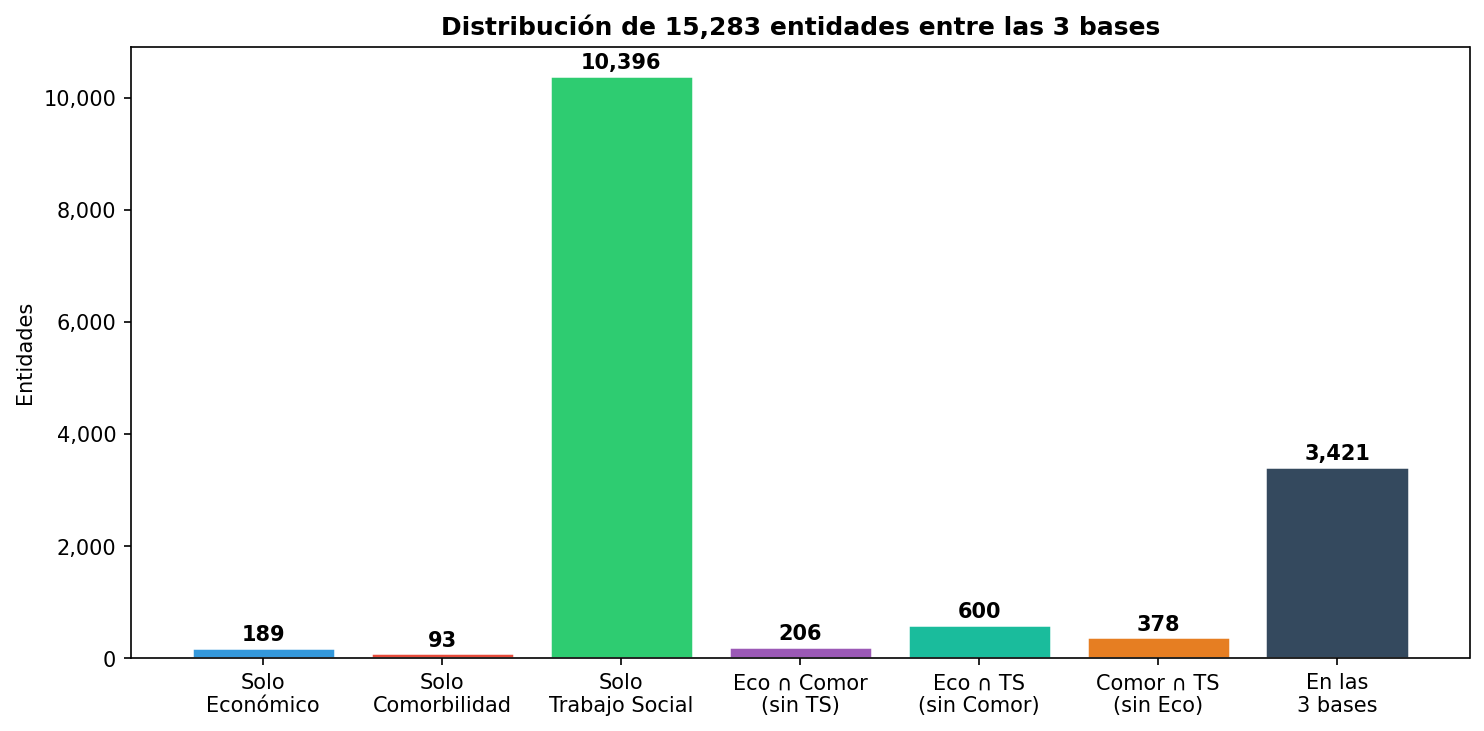
\includegraphics[width=\linewidth]{Figuras/distribucion_entidades.png}
\caption{Distribución de entidades únicas por región}
\label{fig:distribucion_entidades}
\end{figure}

\begin{figure}[H]
\centering
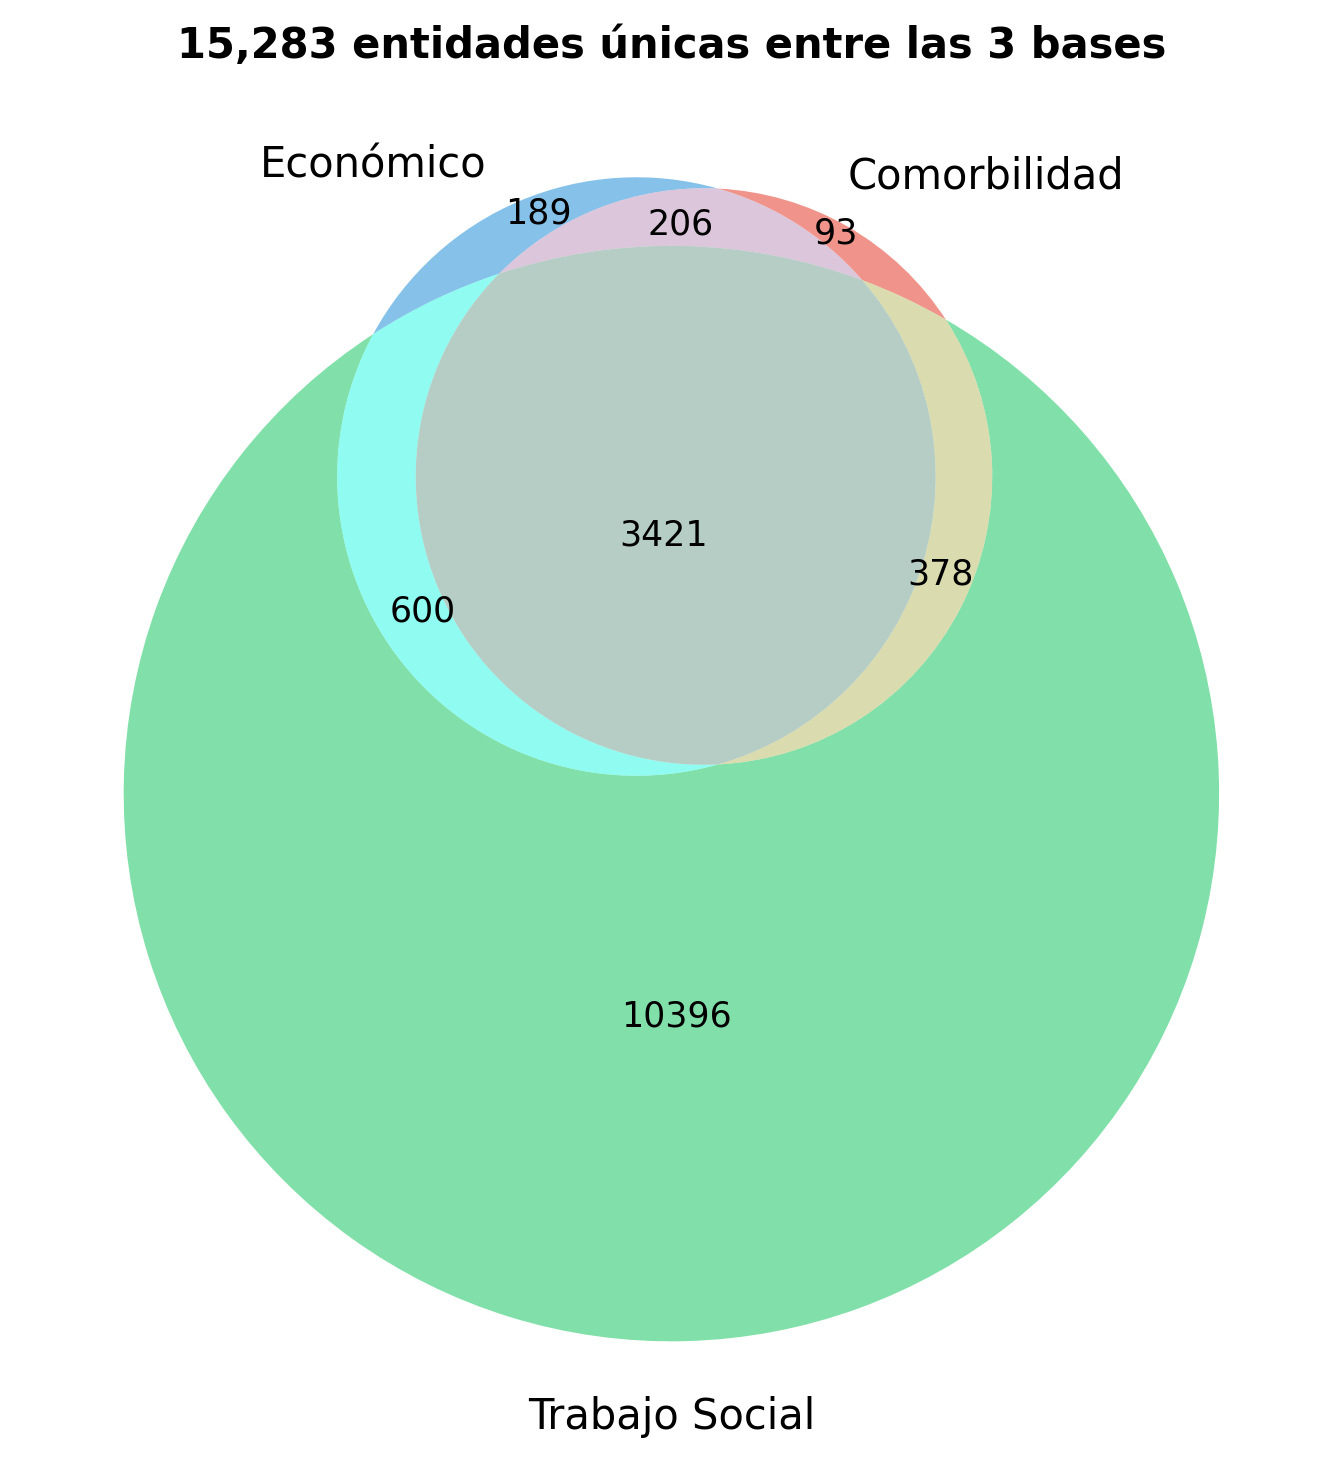
\includegraphics[width=0.75\linewidth]{Figuras/venn_entidades.png}
\caption{Diagrama de Venn: distribución de entidades entre las tres bases}
\label{fig:venn_entidades}
\end{figure}

La tabla~\ref{tab:sintesis_espacios} condensa el resultado completo de la vinculación oficial en dos paneles: las métricas a nivel de pares y las métricas a nivel de entidades.

\begin{table}[H]
\centering
\small
\caption{Síntesis del espacio de búsqueda y entidades vinculables}
\label{tab:sintesis_espacios}
\textbf{Pares de comparación}\\[2pt]
\begin{tabular}{lr}
\toprule
\textbf{Métrica} & \textbf{Valor} \\
\midrule
Espacio total cross-CSV               & 151,648,056 \\
Candidatos (vinculación oficial)      &      11,487 \\
\quad Llave exacta                    &       9,855 \\
\quad Métrica clásica                 &       1,118 \\
\quad Revisión manual                 &         514 \\
Positivos confirmados                 &      11,466 \\
Negativos confirmados                 &          21 \\
\bottomrule
\end{tabular}

\vspace{12pt}

\textbf{Entidades únicas}\\[2pt]
\begin{tabular}{lr}
\toprule
\textbf{Métrica} & \textbf{Valor} \\
\midrule
Registros totales (3 bases)            & 23,706 \\
Entidades únicas                        & 15,283 \\
Solo en una base                        & 10,678 \\
Vinculables (en $\geq$2 bases)          &  4,605 \\
$\bullet$ En exactamente 2 bases        &  1,184 \\
$\bullet$ En las 3 bases                &  3,421 \\
\bottomrule
\end{tabular}
\end{table}

Es importante señalar que este conjunto etiquetado constituye un \textit{silver standard}, no una verdad absoluta. Su construcción depende del número de expediente como filtro primario, lo que implica que cualquier paciente cuyo expediente difiera entre fuentes queda excluido de los candidatos, incluso si su nombre es semánticamente similar. Esta limitación es inherente al enfoque determinístico y motiva la transición hacia un modelo basado en representaciones semánticas, descrito en el Capítulo~4.

\section{Limitaciones}
\label{sec:limitaciones}

El pipeline descrito en las secciones anteriores operó bajo un esquema determinístico basado en reglas explícitas: filtrado por expediente, normalización de nombres, métricas de similitud clásica y revisión manual. Este enfoque fue suficiente para generar el \textit{silver standard}, pero dejó al descubierto tres limitaciones estructurales que motivan un cambio de paradigma.

La primera y más crítica es la \textbf{dependencia del número de expediente como filtro de candidatos}. Cualquier paciente cuyo expediente difiera entre fuentes queda automáticamente excluido del espacio de búsqueda, incluso si su nombre es semánticamente similar. El caso de los 80 registros con \texttt{EXP} nulo en Económico tratados como excepción mediante cruce por nombre evidencia esta fragilidad: un volumen mayor de expedientes faltantes habría requerido un enfoque diferente. La cobertura real del ground truth podría ser ligeramente superior a las 4,605 entidades vinculadas reportadas, pero el método determinístico no puede recuperar esos casos sin ampliar el filtro.

La segunda limitación es la \textbf{colisión de identificadores y el riesgo de falsos positivos por normalización}. En Económico se detectaron 6 expedientes asignados a nombres completamente distintos, lo que significa que un join por expediente sin validación cruzada genera pares espurios. Por otra parte, el ordenamiento alfabético de tokens ---necesario para resolver la diferencia de formato entre Comorbilidad y Económico--- introduce un riesgo: dos personas con los mismos apellidos y nombres, pero en orden diferente, colapsarían a la misma secuencia normalizada. En una base hospitalaria con apellidos frecuentes como García, López o Martínez este riesgo no es despreciable; aunque el expediente actúa como primer filtro, y la revisión manual confirmó 21 negativos explícitos, la prevención de este tipo de errores no puede garantizarse con reglas rígidas.

La tercera limitación es la \textbf{heterogeneidad estructural que impide la comparación directa del registro completo columna a columna}. Una misma variable ---el diagnóstico del paciente--- se representa como texto libre con codificación CIE-10 en Comorbilidad, como categórica de baja cardinalidad en Económico y como texto libre sin codificación en Trabajo Social. Las variables socioeconómicas como escolaridad u ocupación difieren incluso en el vocabulario: Económico emplea catálogos controlados mientras que Trabajo Social las captura como texto libre. Un esquema relacional tradicional requeriría armonizar todas estas representaciones antes de cualquier consulta, lo que resulta inviable cuando los sistemas de origen evolucionan de forma independiente, pero más interesante aún, cuando la información de un mismo paciente queda fragmentada en múltiples fuentes que no comparten el mismo esquema, algoritmos de comparación sintáctica como Jaro-Winkler o Levenshtein no pueden aplicarse de forma directa pues sus puntajes rara vez coinciden de forma consistente y requieren reglas condicionales que crecen en complejidad con cada nueva fuente haciendo que el proceso de ligado sea cada vez más frágil y costoso, llevando un mayor número de casos a revisión manual que podrían resolverse de forma automática si se contara con un modelo de \textbf{comparación semántica}.

Estas limitaciones comparten una causa común: el enfoque opera sobre la \textbf{representación tabular} de los datos, donde cada columna tiene un formato, un orden y un vocabulario definidos por el sistema de origen. La información del mismo paciente queda fragmentada en esquemas inconexos que solo pueden reconciliarse mediante  intervención humana para resolver casos ambiguos.

La alternativa que se explora en el Capítulo~4 consiste en trascender la representación tabular y comparación sintáctica y operar sobre una \textbf{abstracción semántica} del paciente: representar cada registro como un conjunto de \textbf{bloques de información comparables} (diagnóstico clínico, perfil demográfico, situación socioeconómica) independientemente de cómo estén codificados en la base original, y comparar los registros completos mediante representaciones vectoriales aprendidas. Este cambio de paradigma, de la comparación de caracteres en cada columna a la comparación semántica de entidades, es el núcleo metodológico de la propuesta en el siguiente capítulo.
\chapter{Metodología}
% ==============================================================================
% 4.1 BLOQUES SEMÁNTICOS
% ==============================================================================
\section{Definición y estructuración de bloques semánticos}
\label{sec:bloques_semanticos}

El capítulo anterior evidenció tres limitaciones estructurales del enfoque determinístico y sintáctico:

\begin{itemize}
    \item La dependencia del expediente como primer filtro en ausencia de identificadores únicos confiables.
    \item El riesgo de falsos positivos y falsos negativos inducido por la ambigüedad de la captura manual en los nombres y apellidos, que no resuelve la normalización.
    \item La heterogeneidad estructural que impide comparar directamente los registros completos columna a columna entre bases de datos distintas.
\end{itemize}

La más crítica para el diseño de un sistema de ligado automático es la tercera: una misma variable real (el diagnóstico del paciente, su ocupación, su nivel socioeconómico) se representa en cada sistema del INER con esquemas, vocabularios y formatos distintos. Comparar caracteres entre campos que no comparten ni nombre, ni tipo, ni codificación es un callejón sin salida metodológico. La alternativa metodológica que se propone en este capítulo consiste en trascender la representación tabular y operar sobre una \textbf{abstracción semántica} del paciente, donde la información del registro quede representada de manera uniforme y comparable entre bases de datos.

Para ello, se define el concepto de \textbf{bloque semántico} como una agrupación lógica de atributos que comparten un eje de información común, independientemente de la nomenclatura u organización de la base de datos de origen. Cada bloque se materializa en una fuente particular mediante un \textit{soporte}, que es el subconjunto de columnas que lo implementan en esa base específica.

La noción de bloque semántico puede entenderse por analogía con las modalidades de un modelo multimodal. Por ejemplo, en un sistema de clasificación musical, la calidad de la predicción mejora cuando el modelo dispone simultáneamente de la señal de audio, la letra de la canción y el video oficial. Cada una de estas fuentes ofrece una vista parcial de la misma realidad subyacente, y su combinación enriquece la representación que el modelo puede aprender. Sin embargo, no toda canción tiene video oficial; algunas tienen letra, otras no. Un modelo multimodal robusto debe operar con las modalidades disponibles en cada caso, sin depender de que todas estén siempre presentes.

Los bloques semánticos cumplen el mismo rol en el dominio de resolución de entidades en el ámbito clínico. \texttt{[BLK\_ID]} es una modalidad que identifica al paciente, \texttt{[BLK\_CLIN]} es otra que caracteriza su perfil clínico, \texttt{[BLK\_GEO]} otra con información extra, y así sucesivamente. Cada base de datos del INER implementa un subconjunto distinto de estas modalidades: Comorbilidad carece de \texttt{[BLK\_GEO]} y \texttt{[BLK\_SOCIO]} por diseño, del mismo modo que una canción puede carecer de video oficial. Cuando el paciente es atendido en múltiples servicios, sus modalidades se distribuyen entre los sistemas, y es tarea del modelo de ligado reconstruir la unidad de la entidad a partir de las piezas disponibles. La serialización basada en bloques, que se detalla en la Sección~\ref{sec:early_fusion}, materializa esta filosofía: cada registro se representa únicamente con los bloques que posee, produciendo secuencias de longitud variable que reflejan fielmente la información presente sin imputación ni relleno.

% Diagrama: Bloques semánticos como modalidades del paciente
\begin{figure}[H]
\centering
\begin{tikzpicture}[
    cell/.style={align=center, font=\tiny\ttfamily},
    rowbox/.style={draw, rounded corners=1pt, fill=white, inner sep=5pt},
    bloc/.style={draw, rounded corners=3pt, inner sep=2pt},
    rowlabel/.style={anchor=east, font=\footnotesize\sffamily},
    tab/.style={draw, rounded corners=1pt, fill=white, inner xsep=4pt, inner ysep=1pt, font=\scriptsize\sffamily\bfseries}]

\definecolor{cID}{HTML}{4A90D9}
\definecolor{cCLIN}{HTML}{E74C3C}
\definecolor{cGEO}{HTML}{2ECC71}
\definecolor{cSOCIO}{HTML}{F39C12}
\definecolor{cADMIN}{HTML}{9B59B6}

\pgfmathsetmacro{\cw}{2.4}
\pgfmathsetmacro{\cs}{0.2}
\pgfmathsetmacro{\rh}{1.2}
\pgfmathsetmacro{\rs}{0.2}

\pgfmathsetmacro{\xA}{0}
\pgfmathsetmacro{\xB}{\cw+\cs}
\pgfmathsetmacro{\xC}{2*(\cw+\cs)}
\pgfmathsetmacro{\xD}{3*(\cw+\cs)}
\pgfmathsetmacro{\xE}{4*(\cw+\cs)}
\pgfmathsetmacro{\tw}{5*\cw+4*\cs}
\pgfmathsetmacro{\bw}{\cw}
\pgfmathsetmacro{\bh}{3*\rh+2*\rs+0.3}

\pgfmathsetmacro{\yA}{0}
\pgfmathsetmacro{\yB}{-\rh-\rs}
\pgfmathsetmacro{\yC}{-2*\rh-2*\rs}

% BARRAS VERTICALES (bloques)
\node[bloc, fill=cID!10,   minimum width=\bw*1cm, minimum height=\bh*1cm] at (\xA*1cm, 0) {};
\node[bloc, fill=cCLIN!10, minimum width=\bw*1cm, minimum height=\bh*1cm] at (\xB*1cm, 0) {};
\node[bloc, fill=cGEO!10,  minimum width=\bw*1cm, minimum height=\bh*1cm] at (\xC*1cm, 0) {};
\node[bloc, fill=cSOCIO!10,minimum width=\bw*1cm, minimum height=\bh*1cm] at (\xD*1cm, 0) {};
\node[bloc, fill=cADMIN!10,minimum width=\bw*1cm, minimum height=\bh*1cm] at (\xE*1cm, 0) {};

% Etiquetas de bloques (arriba)
\node[above=2mm, font=\small\ttfamily\bfseries] at (\xA*1cm, 0.5*\bh*1cm) {\texttt{[BLK\_ID]}};
\node[above=2mm, font=\small\ttfamily\bfseries] at (\xB*1cm, 0.5*\bh*1cm) {\texttt{[BLK\_CLIN]}};
\node[above=2mm, font=\small\ttfamily\bfseries] at (\xC*1cm, 0.5*\bh*1cm) {\texttt{[BLK\_GEO]}};
\node[above=2mm, font=\small\ttfamily\bfseries] at (\xD*1cm, 0.5*\bh*1cm) {\texttt{[BLK\_SOCIO]}};
\node[above=2mm, font=\small\ttfamily\bfseries] at (\xE*1cm, 0.5*\bh*1cm) {\texttt{[BLK\_ADMIN]}};

% Renglón 1: Comorbilidad
\node[rowbox, minimum width=\tw*1cm, minimum height=\rh*1cm] at (0.5*\tw*1cm, \yA*1cm) {};
\node[tab, anchor=south] at (0.5*\tw*1cm, \yA*1cm + 0.5*\rh*1cm + 0.12cm) {Comorbilidad};
\node[cell] at (\xA*1cm, \yA*1cm) {nombre};
\node[cell] at (\xB*1cm, \yA*1cm) {diagnósticos\\comorbilidades};
\node[cell, text=gray!40] at (\xC*1cm, \yA*1cm) {---};
\node[cell, text=gray!40] at (\xD*1cm, \yA*1cm) {---};
\node[cell] at (\xE*1cm, \yA*1cm) {expediente\\fechas};

% Renglón 2: Económico
\node[rowbox, minimum width=\tw*1cm, minimum height=\rh*1cm] at (0.5*\tw*1cm, \yB*1cm) {};
\node[tab, anchor=south] at (0.5*\tw*1cm, \yB*1cm + 0.5*\rh*1cm + 0.12cm) {Económico};
\node[cell] at (\xA*1cm, \yB*1cm) {nombre\\edad};
\node[cell] at (\xB*1cm, \yB*1cm) {resultado\\etiq\_covid};
\node[cell] at (\xC*1cm, \yB*1cm) {estado\\municipio};
\node[cell] at (\xD*1cm, \yB*1cm) {escolaridad\\ocupación};
\node[cell] at (\xE*1cm, \yB*1cm) {expediente\\estancia\\gastos};

% Renglón 3: Trabajo Social
\node[rowbox, minimum width=\tw*1cm, minimum height=\rh*1cm] at (0.5*\tw*1cm, \yC*1cm) {};
\node[tab, anchor=south] at (0.5*\tw*1cm, \yC*1cm + 0.5*\rh*1cm + 0.12cm) {T. Social};
\node[cell] at (\xA*1cm, \yC*1cm) {apellidos\\nombre\\fecha\_nac};
\node[cell] at (\xB*1cm, \yC*1cm) {diagnóstico};
\node[cell] at (\xC*1cm, \yC*1cm) {delegación\\estado};
\node[cell] at (\xD*1cm, \yC*1cm) {escolaridad\\ocupación\\nivel};
\node[cell] at (\xE*1cm, \yC*1cm) {expediente\\historia\\fecha\_elab};

\end{tikzpicture}
\caption{Bloques semánticos como modalidades. Las columnas verticales representan los cinco bloques;
las franjas horizontales son registros de cada base. Las intersecciones muestran ejemplos del soporte;
las celdas vacías (\texttt{---}) indican bloques ausentes por diseño.}
\label{fig:bloques_modalidades}
\end{figure}


El análisis de los tres sistemas del INER, documentado en el Anexo de Bloques Semánticos, identificó cinco bloques que cubren la totalidad de la información de los pacientes. La Tabla~\ref{tab:columnas_por_bloque_comparativo} muestra el mapeo completo de columnas a bloques para cada fuente.

\begin{table}[H]
\centering
\caption{Columnas por bloque semántico — comparativa entre fuentes}
\label{tab:columnas_por_bloque_comparativo}
\small
\resizebox{\linewidth}{!}{%
\begin{tabular}{>{\raggedright\arraybackslash}p{3cm}
                >{\raggedright\arraybackslash}p{5.5cm}
                >{\raggedright\arraybackslash}p{5.5cm}
                >{\raggedright\arraybackslash}p{5.5cm}}
\toprule
\textbf{Bloque semántico} & \textbf{Comorbilidad} & \textbf{Económico} & \textbf{Trabajo Social} \\
\midrule
\texttt{[BLK\_ID]}
  & \texttt{nombre}
  & \texttt{NOMBRE\_DEL\_PACIENTE}, \texttt{SEXO}, \texttt{EDAD}, \texttt{GRUPO\_EDAD}
  & \texttt{APELLIDO PATERNO}, \texttt{APELLIDO MATERNO}, \texttt{NOMBRE}, \texttt{EDAD}, \texttt{FECHA DE NACIMIENTO}, \texttt{GENERO} \\
\midrule
\texttt{[BLK\_CLIN]}
  & \texttt{diagnosticoprincipal}, \texttt{diagnostico2}, \texttt{diagnostico3}, \texttt{diagnostico4}, \texttt{cie10}, \texttt{cie102}, \texttt{cie103}, \texttt{cie104}, \texttt{dx2}, \texttt{dx3}, \texttt{dx4}, \texttt{comorbi}, \texttt{comorbicv}, \texttt{obesidad}, \texttt{obesidad1}, \texttt{cardiopatia}, \texttt{diabetes}, \texttt{nefropatia}, \texttt{eaperge}, \texttt{tephap}
  & \texttt{RESULTADO}, \texttt{ETIQUETAS\_COVID}, \texttt{MOTIVO\_DE\_EGRESO}
  & \texttt{DIAGNOSTICO} \\
\midrule
\texttt{[BLK\_GEO]}
  & ---
  & \texttt{ESTADO\_RESIDENCIA}, \texttt{MUNICIPIO\_RESIDENCIA}, \texttt{CLAVE GEOESTADISTICA} (estatal y municipal)
  & \texttt{DELEGACIÓN O MUNICIPIO PERMANENTE}, \texttt{ESTADO / PAIS PERMANENTE} \\
\midrule
\texttt{[BLK\_SOCIO]}
  & ---
  & \texttt{ESCOLARIDAD}, \texttt{OCUPACION}, \texttt{DERECHOHABIENTE Y/O BENEFICIARIO}, \texttt{NIVEL\_SOCIOECONOMICO}, \texttt{VULNERABILIDAD\_SOCIOECONOMICA}
  & \texttt{ESCOLARIDAD}, \texttt{OCUPACIÓN}, \texttt{DERECHOHABIENTE Y/O BENEFICIARIO}, \texttt{TOTAL DE PUNTOS}, \texttt{NIVEL SOCIOECONÓMICO} \\
\midrule
\texttt{[BLK\_ADMIN]}
  & \texttt{expediente}, \texttt{fechaing}, \texttt{fechaegr}
  & \texttt{EXP}, \texttt{DIAS\_ESTANCIA}, \texttt{FECHA\_INGRESO\_INER}, \texttt{FECHA\_DE\_ALTA\_MEJORIA}, \texttt{TOTAL\_DE\_INGRESOS}, \texttt{TOTAL\_DE\_EGRESOS}, \texttt{GASTO\_TOTAL}, \texttt{GASTO\_DIARIO}
  & \texttt{EXPEDIENTE}, \texttt{NO. HISTORIA}, \texttt{FECHA DE ELABORACIÓN}, \texttt{AÑO}, \texttt{FILA} \\
\bottomrule
\end{tabular}}
\end{table}

La tabla revela dos formas de heterogeneidad. La primera es cuantitativa: un mismo bloque tiene distinto número de columnas según la fuente. \texttt{[BLK\_ID]} va de 1 columna en Comorbilidad a 6 en Trabajo Social; \texttt{[BLK\_CLIN]} va de 20 columnas en Comorbilidad a 1 en Trabajo Social. La segunda es cualitativa: los soportes no solo difieren en tamaño, sino también en el vocabulario y la granularidad de los datos. En \texttt{[BLK\_GEO]}, Económico desglosa estado y municipio en columnas separadas más claves geoestadísticas oficiales, mientras que Trabajo Social los agrupa en dos campos descriptivos; en \texttt{[BLK\_SOCIO]}, Económico incluye \texttt{VULNERABILIDAD\_SOCIOECONOMICA} como columna explícita, mientras que Trabajo Social la aproxima mediante \texttt{TOTAL DE PUNTOS}.

La segunda dimensión de heterogeneidad es la cobertura: no todas las fuentes implementan todos los bloques. Comorbilidad, al ser una base enfocada exclusivamente en el perfil clínico del paciente, carece por completo de los bloques \texttt{[BLK\_GEO]} y \texttt{[BLK\_SOCIO]}. Esto implica que un registro de Comorbilidad, por definición, nunca contará con información geográfica ni socioeconómica, independientemente de si el paciente la tiene registrada en otros sistemas. La Tabla~\ref{tab:bloques_completitud_comparativo} resume la completitud de cada bloque por fuente.

\begin{table}[H]
\centering
\caption{Completitud por bloque semántico — comparativa}
\label{tab:bloques_completitud_comparativo}
\small
\resizebox{\linewidth}{!}{%
\begin{tabular}{>{\raggedright\arraybackslash}p{2.8cm}
                >{\centering\arraybackslash}p{1.4cm}
                >{\centering\arraybackslash}p{2.0cm}
                >{\centering\arraybackslash}p{1.4cm}
                >{\centering\arraybackslash}p{2.0cm}
                >{\centering\arraybackslash}p{1.4cm}
                >{\centering\arraybackslash}p{2.0cm}}
\toprule
\textbf{Bloque} & \multicolumn{2}{c}{\textbf{Comorbilidad}} & \multicolumn{2}{c}{\textbf{Económico}} & \multicolumn{2}{c}{\textbf{Trabajo Social}} \\
\cmidrule(lr){2-3}\cmidrule(lr){4-5}\cmidrule(lr){6-7}
 & \textbf{Cols.} & \textbf{\% Completo} & \textbf{Cols.} & \textbf{\% Completo} & \textbf{Cols.} & \textbf{\% Completo} \\
\midrule
\texttt{[BLK\_ID]}    & 1  & 100.0\% & 4  & 99.8\%  & 6  & 94.7\% \\
\texttt{[BLK\_CLIN]}  & 20 & 10.8\%  & 3  & 33.4\%  & 1  & 38.7\% \\
\texttt{[BLK\_GEO]}   & --- & ---    & 4  & 98.8\%  & 2  & 98.3\% \\
\texttt{[BLK\_SOCIO]} & --- & ---    & 5  & 35.2\%  & 5  & 93.8\% \\
\texttt{[BLK\_ADMIN]} & 3  & 100.0\% & 8  & 79.4\%  & 5  & 98.2\% \\
\bottomrule
\end{tabular}}
\end{table}
{\footnotesize\textit{\textbf{\% Completo}:} porcentaje de registros en los que \emph{todas} las columnas del bloque son no nulas. Un único campo nulo dentro del bloque afecta la completitud del bloque.}

Esta tabla introduce una tercera capa de heterogeneidad: incluso cuando un bloque existe en una fuente, su completitud varía drásticamente. \texttt{[BLK\_CLIN]} es el caso más extremo: en Comorbilidad solo el 10.8\% de los registros tienen las 20 columnas clínicas completas, debido a la estructura jerárquica de diagnósticos (un paciente puede tener de 1 a 4 diagnósticos, y las columnas \texttt{diagnostico2} a \texttt{diagnostico4} quedan nulas si no aplican). En Económico, la completitud del mismo bloque es del 33.4\%, lastrada por la incorporación tardía de \texttt{ETIQUETAS\_COVID} (66.5\% de registros con este campo nulo). En Trabajo Social, \texttt{DIAGNOSTICO} es un campo auxiliar que solo se llenó para pacientes COVID, resultando en 38.7\% de completitud. Por el contrario, \texttt{[BLK\_ID]} es robusto en las tres fuentes (94.7\% a 100\%), y \texttt{[BLK\_ADMIN]} también se mantiene alto (79.4\% a 100\%).

Tres patrones adicionales merecen atención. Primero, \texttt{[BLK\_SOCIO]} es fuerte en Trabajo Social (93.8\%) pero débil en Económico (35.2\%), donde \texttt{OCUPACION} es el principal responsable de la incompletitud (64.8\% nulos). Segundo, Comorbilidad tiene el \texttt{[BLK\_CLIN]} más rico en número de columnas (20) pero el más fragmentado por nulos; Trabajo Social tiene el más escaso en columnas (1) pero el más limpio en cobertura relativa. Tercero, un bloque ausente (\texttt{---} en la tabla) no es un caso de datos faltantes: es una ausencia estructural por diseño del sistema de origen.

Esta heterogeneidad de cobertura no es un obstáculo para el enfoque propuesto, sino precisamente la razón que lo motiva. La serialización basada en bloques, que se detalla en la Sección~\ref{sec:early_fusion}, simplemente omite los bloques ausentes en cada registro y serializa únicamente los presentes, produciendo secuencias de longitud variable que reflejan fielmente la información disponible sin necesidad de imputación ni relleno.


% ==============================================================================
% 4.2 ARQUITECTURA GENERAL Y EL PROBLEMA O(N^2)
% ==============================================================================
\section{Arquitectura general del sistema: \textit{Retrieve \& Re-rank}}

Los modelos de lenguaje pre-entrenados como BERT (\textit{Bidirectional Encoder Representations from Transformers}) ofrecen una vía para abordar la heterogeneidad estructural descrita en la sección anterior. Su representación textual permite procesar registros con atributos faltantes sin requerir imputación de datos; sin embargo, esto no garantiza una robustez intrínseca ante la ausencia de información, pues el impacto depende del patrón de faltantes y de la capacidad del modelo para discriminar con los atributos disponibles. Su aplicación directa al problema de ligado de registros enfrenta además una barrera computacional inmediata: la comparación exhaustiva.

Dadas dos bases de datos $A$ y $B$ con $n$ y $m$ registros respectivamente, el enfoque ingenuo de evaluar todos los pares posibles tiene complejidad $\mathcal{O}(n \cdot m)$. En el caso concreto del INER, los volúmenes de las tres fuentes (4,278 registros en Comorbilidad, 4,632 en Económico y 14,796 en Trabajo Social) generan productos cartesianos del orden de decenas de millones de pares. Por ejemplo, alinear Comorbilidad contra Económico produce aproximadamente 19.8 millones de combinaciones, y Comorbilidad contra Trabajo Social alcanza 63.3 millones. Ejecutar un Transformer profundo sobre cada par es computacionalmente inviable, incluso con aceleración por GPU.

% Diagrama del espacio de búsqueda O(n^3)
% Tres bases de datos como ejes del cubo; cada cara = producto cartesiano
\providecolor{csvComorbilidad}{HTML}{E89D9D}
\providecolor{csvEconomico}{HTML}{A8C8E0}
\providecolor{csvTrabajoSocial}{HTML}{A8D5BA}
\providecolor{petroleo}{HTML}{3B5366}
\providecolor{vinoCIMAT}{HTML}{7A2237}
\begin{center}
\begin{tikzpicture}[
  scale=1.8,
  font=\footnotesize,
  arr/.style={->, >=Stealth, line width=0.8pt}
]
  % Ángulo de proyección
  \pgfmathsetmacro{\ca}{cos(20)}
  \pgfmathsetmacro{\sa}{sin(20)}
  \pgfmathsetmacro{\sx}{2.0}
  \pgfmathsetmacro{\sy}{2.2}
  \pgfmathsetmacro{\sz}{3.5}

  % Coordenadas 3D → 2D
  \coordinate (O)   at (0, 0);
  \coordinate (X)   at ({\sx*\ca}, {\sx*\sa});
  \coordinate (Y)   at ({\sy*\ca}, {-\sy*\sa});
  \coordinate (Z)   at (0, \sz);
  \coordinate (XY)  at ({\sx*\ca + \sy*\ca}, {\sx*\sa - \sy*\sa});
  \coordinate (XZ)  at ({\sx*\ca}, {\sz + \sx*\sa});
  \coordinate (YZ)  at ({\sy*\ca}, {\sz - \sy*\sa});
  \coordinate (XYZ) at ({\sx*\ca + \sy*\ca}, {\sz + \sx*\sa - \sy*\sa});

  % --- Caras del cubo (en orden inverso para superposición correcta) ---

  % Cara trasera (yz): Económico × T. Social
  \fill[csvEconomico!30] (O) -- (Y) -- (YZ) -- (Z) -- cycle;
  \draw[csvEconomico, line width=1.0pt] (O) -- (Y) -- (YZ) -- (Z) -- cycle;

  % Cara trasera (xz): Comorbilidad × T. Social
  \fill[csvComorbilidad!30] (O) -- (X) -- (XZ) -- (Z) -- cycle;
  \draw[csvComorbilidad, line width=1.0pt] (O) -- (X) -- (XZ) -- (Z) -- cycle;

  % Cara inferior (xy): Comorbilidad × Económico
  \fill[csvTrabajoSocial!30] (O) -- (X) -- (XY) -- (Y) -- cycle;
  \draw[csvTrabajoSocial, line width=1.0pt] (O) -- (X) -- (XY) -- (Y) -- cycle;

  % Aristas de la cara superior (semiocultas, punteadas)
  \draw[csvEconomico, line width=0.6pt, dashed] (X) -- (XZ) -- (XYZ) -- (YZ) -- (Y);
  \draw[csvTrabajoSocial, line width=0.6pt, dashed] (X) -- (XY) -- (Y);
  \draw[csvComorbilidad, line width=0.6pt, dashed] (XZ) -- (XYZ) -- (YZ);

  % --- Flechas de los ejes ---
  \begin{scope}[arr]
    \draw[petroleo] (O) -- ({2.3*\ca}, {2.3*\sa})   node[anchor=south west, petroleo] {Comorbilidad 4,278};
    \draw[vinoCIMAT] (O) -- ({2.5*\ca}, {-2.5*\sa})  node[anchor=north west, vinoCIMAT] {Económico 4,632};
    \draw[petroleo!50!vinoCIMAT] (O) -- (0, 3.7) node[anchor=east, petroleo!50!vinoCIMAT] {Trabajo Social 14,796};
  \end{scope}

  % --- Etiquetas de pares por cara (centroides calculados) ---
  \node[fill=white, inner sep=2pt, font=\small] at ({\sx*\ca/2}, {(\sx*\sa + \sz)/2})     {63.3M pares};
  \node[fill=white, inner sep=2pt, font=\small] at ({\sy*\ca/2}, {(\sz - \sy*\sa)/2})     {68.5M pares};
  \node[fill=white, inner sep=2pt, font=\small] at ({(\sx+\sy)*\ca/2}, {(\sx-\sy)*\sa/2}) {19.8M pares};

  % --- Anotación de complejidad ---
  \node[font=\footnotesize, anchor=north] at ({(\sx+\sy)*\ca/2}, -2.0)
    {Total: $\sim$151.6M pares ($\mathcal{O}(n^3)$)};

\end{tikzpicture}
\captionof{figure}{Espacio de búsqueda del problema de ligado. Cada eje representa una base de datos y cada cara del cubo corresponde al producto cartesiano entre dos fuentes.}
\label{fig:cubo_producto_cartesiano}
\end{center}


La solución propuesta sigue la arquitectura \textit{Retrieve \& Re-rank}, un embudo de dos fases que separa la eficiencia de la profundidad. En la primera fase, un modelo ligero (\textit{Bi-Encoder}) proyecta cada registro a un vector denso de baja dimensión y recupera los $K$ vecinos más cercanos mediante similitud coseno, reduciendo el espacio de búsqueda de $\mathcal{O}(n \cdot m)$ a $\mathcal{O}(n \cdot K)$ con $K \ll m$. En la segunda fase, un modelo profundo (\textit{Cross-Encoder}) examina con atención cruzada únicamente los $K$ pares candidatos por registro y produce una decisión final de ligado.

Esta arquitectura no solo resuelve el problema de escalabilidad, sino que además introduce una división metodológica natural entre las dos fases. El Bi-Encoder optimiza recuperación (\textit{recall}), priorizando no descartar ningún par legítimo, mientras que el Cross-Encoder optimiza precisión (\textit{precision}), discriminando entre los falsos positivos y los verdaderos positivos que el primer filtro no pudo separar. El resultado es un sistema que combina lo mejor de ambos mundos: la eficiencia de una búsqueda de vecinos y la sensibilidad de un clasificador profundo.

% Diagrama de la arquitectura Retrieve & Re-rank
% Adaptado de Presentacion_4/Secciones/01_recap.tex
\providecolor{petroleo}{HTML}{3B5366}
\providecolor{vinoCIMAT}{HTML}{7A2237}
\providecolor{semVerde}{HTML}{4CAF50}
\providecolor{hardNegative}{HTML}{E89D9D}
\begin{center}
\begin{tikzpicture}[
  >={Stealth[length=2.5mm]},
  arr/.style={->, gray!55, dashed, line width=0.9pt},
  every node/.style={font=\footnotesize}
]
  % --- Datos tabulares (3 cards escalonadas) ---
  \filldraw[white, draw=gray!30, line width=0.4pt, rounded corners=2pt] (0.6, -0.7) rectangle (1.8, 0.3);
  \filldraw[white, draw=gray!30, line width=0.4pt, rounded corners=2pt] (0.3, -0.45) rectangle (1.5, 0.55);
  \filldraw[white, draw=gray!40, line width=0.4pt, rounded corners=2pt] (0,   -0.2)  rectangle (1.2, 0.8);
  \node[font=\small\bfseries] at (0.6, 0.3) {Bases};
  \node[font=\footnotesize, anchor=north] at (0.9, -0.85) {de datos};

  % --- Arrow 1 ---
  \draw[arr] (2.0, 0.05) -- (2.7, 0.05);

  % --- Embudo 1: Bi-Encoder (petróleo) ---
  \fill[petroleo] (2.9, -1.1) -- (2.9, 1.1) -- (5.0, 0.45) -- (5.0, -0.45) -- cycle;
  \node[white, font=\footnotesize\bfseries] at (3.95, 0.25) {Bi-Encoder};
  \node[white, font=\footnotesize\itshape]  at (3.95, -0.15) {retrieval};

  % --- Arrow 2 ---
  \draw[arr] (5.2, 0) -- (5.9, 0);

  % --- Box: top-K candidatos ---
  \filldraw[white, draw=petroleo, line width=0.7pt, rounded corners=4pt]
    (6.1, -0.55) rectangle (7.8, 0.55);
  \node[color=petroleo, font=\footnotesize\bfseries] at (6.95, 0.2)  {top-$K$};
  \node[color=petroleo, font=\footnotesize]          at (6.95, -0.2) {candidatos};

  % --- Arrow 3 ---
  \draw[arr] (8.0, 0) -- (8.7, 0);

  % --- Embudo 2: Cross-Encoder (vino) ---
  \fill[vinoCIMAT] (8.9, -0.75) -- (8.9, 0.75) -- (11.7, 0.25) -- (11.7, -0.25) -- cycle;
  \node[white, font=\footnotesize\bfseries] at (10.3, 0.2)  {Cross-Encoder};
  \node[white, font=\footnotesize\itshape]  at (10.3, -0.2) {re-ranking};

  % --- Arrow 4 ---
  \draw[arr] (11.9, 0) -- (12.6, 0);

  % --- Match / No Match (dos pills) ---
  \filldraw[semVerde!75, rounded corners=6pt] (12.8, 0.15) rectangle (14.3, 0.6);
  \node[white, font=\footnotesize\bfseries] at (13.55, 0.37) {Match};

  \filldraw[hardNegative!90, rounded corners=6pt] (12.8, -0.6) rectangle (14.3, -0.15);
  \node[white, font=\footnotesize\bfseries] at (13.55, -0.37) {No Match};
\end{tikzpicture}
\captionof{figure}{Arquitectura \textit{Retrieve \& Re-rank}.}
\label{fig:embudo_arquitectura}
\end{center}


Antes de describir cada fase en detalle, es necesario resolver un problema transversal: los modelos Transformer procesan secuencias de texto, no filas de una base de datos. La siguiente sección aborda el mecanismo de serialización que convierte los registros tabulares del INER en secuencias de texto plano sin perder la estructura semántica de los datos.

% ==============================================================================
% 4.3 EARLY FUSION Y TOKENS (Ahora tiene sentido)
% ==============================================================================
\section{Representación de entradas: Fusión Temprana (\textit{Early Fusion})}
\label{sec:early_fusion}

Para que un Transformer pueda procesar un registro tabular, es necesario traducir la estructura de filas y columnas de las bases de datos a una secuencia lineal de tokens, análoga al texto en lenguaje natural. Esta traducción debe preservar la semántica de los datos y permitir que el modelo aprenda relaciones entre atributos incluso cuando estos provienen de fuentes distintas, con esquemas heterogéneos y un alto porcentaje de valores nulos.

En la sección anterior se definió el concepto de \textbf{bloque semántico} como una abstracción en la que cada registro es la unión de varios bloques de información, cada uno análogo a una modalidad distinta. La propuesta presentada preserva esta estructura mediante una \textbf{serialización} que concatena los bloques semánticos de cada registro, donde cada bloque contiene sus atributos en formato clave-valor. Este enfoque constituye una estrategia de \textit{fusión temprana} (\textit{early fusion}), en la que todos los atributos de un registro se combinan en una sola cadena de texto antes de ser alimentada al modelo. En contraste, la fusión tardía codificaría cada bloque por separado y combinaría las representaciones posteriormente, lo que implicaría una mayor carga computacional y complejidad al requerir un modelo codificador por modalidad.

La ventaja de la fusión temprana, además de la simplicidad en la implementación, es que el mecanismo de atención del Transformer puede modelar las interacciones entre cualquier par de atributos desde la primera capa de manera autónoma, sin requerir ingeniería de características, supuestos sobre importancia relativa de columnas ni depender de valores no nulos en campos específicos.

El formato de serialización sigue una estructura de clave-valor etiquetada mediante tokens especiales adoptada de la arquitectura DITTO~\cite{li2020}. En dicha arquitectura, cada atributo se representa con los tokens \texttt{[COL]} y \texttt{[VAL]} para indicar el inicio del nombre del atributo y de su valor respectivamente, enseñando al modelo la estructura relacional clave-valor. Sobre esta base, este trabajo introduce una extensión jerárquica: los tokens \texttt{[BLK\_ID]}, \texttt{[BLK\_CLIN]}, etc., delimitan los bloques semánticos definidos en la Sección~\ref{sec:bloques_semanticos}, permitiendo que el modelo aprenda la pertenencia de cada atributo a su bloque y pondere la importancia relativa de cada modalidad. Por ejemplo, un registro mínimo con identidad y datos clínicos se serializaría como:

\begin{verbatim}
[BLK_ID] [COL] nombre [VAL] JUAN PEREZ [COL] edad [VAL] 45 [/BLK_ID]
[BLK_CLIN] [COL] diagnostico [VAL] NEUMONIA [/BLK_CLIN]
\end{verbatim}

% Diagrama: Serialización Early Fusion (tabla → secuencia)
% Uso vertical para evitar desbordar página; colores de bloques_modalidades.tex
\providecolor{cID}{HTML}{4A90D9}
\providecolor{cCLIN}{HTML}{E74C3C}
\providecolor{cGEO}{HTML}{2ECC71}
\providecolor{cSOCIO}{HTML}{F39C12}
\providecolor{cADMIN}{HTML}{9B59B6}
\begin{center}
\begin{tikzpicture}[
  cell/.style={font=\small\ttfamily, align=left, inner sep=3pt},
  blk/.style={draw, rounded corners=3pt, inner sep=4pt, outer sep=1pt},
  hdr/.style={font=\small\bfseries\sffamily, anchor=west},
  arrow/.style={->, >=Stealth, thick, gray!60},
  seq/.style={font=\small\ttfamily, align=left, inner sep=2pt},
  tok/.style={font=\small\bfseries, inner sep=1pt},
  ann/.style={font=\footnotesize, gray!70, inner sep=2pt},
]
  % ==================== PANEL SUPERIOR: REGISTRO TABULAR ====================
  % Coordenadas base
  \pgfmathsetmacro{\xL}{0}
  \pgfmathsetmacro{\xM}{3.5}
  \pgfmathsetmacro{\xR}{11}
  \pgfmathsetmacro{\dy}{0.8}
  \pgfmathsetmacro{\yStart}{0}

  % Encabezado panel
  \node[hdr] at (\xL, \yStart) {Registro tabular (Comorbilidad)};

  % Función auxiliar para filas
  \newcommand{\fila}[3]{%
    \node[blk, fill=#1!15, draw=#1] at (\xM, #2) {#3};
  }

  % BLK_ID
  \node[blk, fill=cID!15, draw=cID, minimum width=2.2cm] at (\xL+1.1, \yStart-\dy) {\bfseries\sffamily\color{cID}[BLK\_ID]};
  \fila{cID}{\yStart-2*\dy}{nombre = JUAN PEREZ}
  \fila{cID}{\yStart-3*\dy}{edad = 45}
  \node[blk, fill=cID!15, draw=cID, minimum width=2.2cm] at (\xL+1.1, \yStart-4*\dy) {\bfseries\sffamily\color{cID}[/BLK\_ID]};

  % BLK_CLIN
  \node[blk, fill=cCLIN!15, draw=cCLIN, minimum width=2.2cm] at (\xL+1.1, \yStart-5*\dy) {\bfseries\sffamily\color{cCLIN}[BLK\_CLIN]};
  \fila{cCLIN}{\yStart-6*\dy}{diagnostico = NEUMONIA}
  \fila{cCLIN}{\yStart-7*\dy}{\color{gray!50}diagnostico2 = \textit{(nulo)}}
  \node[blk, fill=cCLIN!15, draw=cCLIN, minimum width=2.2cm] at (\xL+1.1, \yStart-8*\dy) {\bfseries\sffamily\color{cCLIN}[/BLK\_CLIN]};

  % BLK_GEO (ausente)
  \node[blk, fill=gray!10, draw=gray!50, minimum width=2.2cm, dashed] at (\xL+1.1, \yStart-9*\dy) {\bfseries\sffamily\color{gray!60}[BLK\_GEO] (ausente)};
  \node[ann] at (\xR, \yStart-9*\dy) {bloque ausente $\to$ omitido};

  % BLK_SOCIO (ausente)
  \node[blk, fill=gray!10, draw=gray!50, minimum width=2.2cm, dashed] at (\xL+1.1, \yStart-10*\dy) {\bfseries\sffamily\color{gray!60}[BLK\_SOCIO] (ausente)};
  \node[ann] at (\xR, \yStart-10*\dy) {bloque ausente $\to$ omitido};

  % BLK_ADMIN
  \node[blk, fill=cADMIN!15, draw=cADMIN, minimum width=2.2cm] at (\xL+1.1, \yStart-11*\dy) {\bfseries\sffamily\color{cADMIN}[BLK\_ADMIN]};
  \fila{cADMIN}{\yStart-12*\dy}{expediente = 12345}
  \fila{cADMIN}{\yStart-13*\dy}{fechaing = 2020-03-15}
  \node[blk, fill=cADMIN!15, draw=cADMIN, minimum width=2.2cm] at (\xL+1.1, \yStart-14*\dy) {\bfseries\sffamily\color{cADMIN}[/BLK\_ADMIN]};

  % ==================== FLECHA CENTRAL ====================
  \pgfmathsetmacro{\yMid}{\yStart - 7.5*\dy}
  \draw[arrow] (\xR+0.5, \yMid) -- node[fill=white, inner sep=4pt, font=\small\bfseries] {Early Fusion + Serialización} (\xR+2.5, \yMid);

  % ==================== PANEL INFERIOR: SECUENCIA SERIALIZADA ====================
  \pgfmathsetmacro{\xSeq}{\xR+3.5}
  \pgfmathsetmacro{\ySeqStart}{\yStart + 1.5}
  \pgfmathsetmacro{\dySeq}{0.7}

  \node[hdr] at (\xSeq, \ySeqStart) {Secuencia tokenizada};

  % Definir estilos de tokens por bloque
  \newcommand{\tok}[3]{%
    \node[seq, color=#1] at (\xSeq, #2) {#3};
  }

  % BLK_ID
  \tok{cID}{\ySeqStart}{[BLK\_ID]}
  \tok{cID}{\ySeqStart-\dySeq}{[COL] nombre [VAL] JUAN PEREZ}
  \tok{cID}{\ySeqStart-2*\dySeq}{[COL] edad [VAL] 45}
  \tok{cID}{\ySeqStart-3*\dySeq}{[/BLK\_ID]}

  % BLK_CLIN
  \tok{cCLIN}{\ySeqStart-4*\dySeq}{[BLK\_CLIN]}
  \tok{cCLIN}{\ySeqStart-5*\dySeq}{[COL] diagnostico [VAL] NEUMONIA}
  \tok{cCLIN}{\ySeqStart-6*\dySeq}{[/BLK\_CLIN]}
  \node[ann, color=cCLIN] at (\xSeq+5.5, \ySeqStart-5*\dySeq) {diagnostico2 omitido (nulo)};

  % BLK_ADMIN
  \tok{cADMIN}{\ySeqStart-7*\dySeq}{[BLK\_ADMIN]}
  \tok{cADMIN}{\ySeqStart-8*\dySeq}{[COL] expediente [VAL] 12345}
  \tok{cADMIN}{\ySeqStart-9*\dySeq}{[COL] fechaing [VAL] 2020-03-15}
  \tok{cADMIN}{\ySeqStart-10*\dySeq}{[/BLK\_ADMIN]}

  % Leyenda de bloques ausentes
  \node[ann] at (\xSeq, \ySeqStart-11*\dySeq) {[BLK\_GEO], [BLK\_SOCIO] omitidos (bloques ausentes por diseño)};

\end{tikzpicture}
\captionof{figure}{Proceso de serialización \textit{early fusion}: registro tabular $\to$ secuencia de tokens con bloques semánticos coloreados.}
\label{fig:serializacion_early_fusion}
\end{center}

La literatura de DITTO propone además dos mecanismos complementarios: la \textit{tipificación de segmentos} (\textit{span typing}), que envuelve campos críticos como identificadores únicos o fechas con etiquetas especiales (\texttt{<UID>}, \texttt{<DATE>}) para forzar la atención sobre coincidencias exactas, y la \textit{normalización de segmentos} (\textit{span normalization}), que estandariza formatos variables (fechas, numéricos) a una representación canónica~\cite{li2020}. Ambos mecanismos fueron considerados durante el diseño, pero se descartaron en la implementación final: en los registros del INER, la variabilidad de formato en esos campos es limitada y el modelo puede aprender las correspondencias sintácticas mediante el entrenamiento contrastivo que se describe en las secciones siguientes, sin necesidad de etiquetas adicionales.

Para evaluar las decisiones de representación se generaron cuatro variantes. La literatura de DITTO propone el token especial \texttt{[VAL\_NULL]} para señalar ausencias~\cite{li2020}; en este trabajo, las variantes que conservan nulos utilizan el marcador textual \texttt{NULL}.
\begin{itemize}
    \item \texttt{tok\_keepnull}: utiliza tokens especiales estructurales y conserva los valores nulos como \texttt{NULL}.
    \item \texttt{tok\_skipnull}: utiliza los mismos tokens especiales y omite las columnas con valores nulos; un bloque vacío también se omite.
    \item \texttt{notok\_keepnull}: emplea el formato plano \texttt{columna: valor}, sin tokens especiales, y conserva los valores nulos como \texttt{NULL}.
    \item \texttt{notok\_skipnull}: emplea el mismo formato plano sin tokens especiales y omite las columnas con valores nulos.
\end{itemize}

En las variantes \texttt{tok}, los siete tokens especiales estructurales (\texttt{[BLK\_ID]}, \texttt{[BLK\_CLIN]}, \texttt{[BLK\_GEO]}, \texttt{[BLK\_SOCIO]}, \texttt{[BLK\_ADMIN]}, \texttt{[COL]} y \texttt{[VAL]}) se registraron en el vocabulario del tokenizador y se redimensionó la capa de \textit{embeddings} del modelo. Para evitar que la inicialización aleatoria de estos nuevos vectores introdujera ruido, cada token se inicializó como el centroide semántico de un conjunto de palabras ancla en español (por ejemplo, \texttt{[BLK\_ID]} se inicializó a partir de ``identidad'', ``identificación'', ``paciente''), siguiendo una estrategia de \textit{warm initialization}.

Esta representación tiene tres propiedades deseables. Primera, preserva la semántica de los bloques y permite que el modelo pondere su importancia mediante la atención. Segunda, la estructura clave-valor hace explícita la correspondencia entre columnas de distintas fuentes aunque los nombres difieran; el modelo aprende que \texttt{[COL] nombre} en una base y \texttt{[COL] NOMBRE\_DEL\_PACIENTE} en otra apuntan al mismo tipo de información. Tercera, la serialización es completamente determinista e independiente del orden de las columnas originales, lo que garantiza reproducibilidad.

Dado que los modelos Transformer imponen un límite estricto de tokens de entrada, se midió la longitud de los registros de cada variante con el tokenizador registrado del Bi-Encoder canónico, incluyendo los tokens de inicio y separación y sin aplicar truncamiento. La Tabla~\ref{tab:tokens_comparativo} resume los 23,706 registros de cada variante.

\begin{table}[H]
\centering
\caption{Longitud real de los registros serializados por variante, medida con el tokenizador del Bi-Encoder}
\label{tab:tokens_comparativo}
\small
\begin{tabular}{>{\raggedright\arraybackslash}p{5cm}
                >{\centering\arraybackslash}p{2.5cm}
                >{\centering\arraybackslash}p{2.5cm}
                >{\centering\arraybackslash}p{2.5cm}}
\toprule
\textbf{Variante} & \textbf{Mínimo} & \textbf{Promedio} & \textbf{Máximo} \\
\midrule
\texttt{tok\_keepnull}   & 122 & 234.7 & 368 \\
\texttt{tok\_skipnull}   & 118 & 223.1 & 363 \\
\texttt{notok\_keepnull} & 111 & 213.0 & 339 \\
\texttt{notok\_skipnull} & 100 & 202.6 & 334 \\
\bottomrule
\end{tabular}
\end{table}

Ningún registro individual supera el límite de 384 tokens utilizado por el Bi-Encoder, por lo que esta etapa no aplica truncamiento. Como era esperable, los tokens especiales estructurales incrementan la longitud de las secuencias: al comparar variantes con el mismo tratamiento de nulos, las variantes con tokens son más largas que sus equivalentes sin tokens. Por otra parte, omitir los valores nulos reduce la longitud promedio respecto a conservarlos, tanto con tokens como sin ellos.

% ==============================================================================
% 4.4 FASE 1: SBERT
% ==============================================================================
\section{Fase 1: Recuperación eficiente (\textit{Retrieval}) mediante Bi-Encoders}
\label{sec:bi_encoder}

La primera fase del embudo \textit{Retrieve \& Re-rank} emplea una arquitectura \textbf{Bi-Encoder} basada en \textit{Sentence-BERT} (SBERT)~\cite{reimers2019}. A diferencia de un Transformer convencional que procesa un par de secuencias de forma conjunta, el Bi-Encoder utiliza dos codificadores con pesos compartidos (arquitectura siamesa) que procesan cada registro de forma independiente. Cada registro serializado se pasa por el mismo Transformer pre-entrenado y la representación de la secuencia completa se condensa en un vector denso mediante \textit{mean pooling} sobre los tokens de salida de la última capa oculta.

\subsection{Arquitectura y configuración}

La Tabla~\ref{tab:biencoder_config} resume la configuración utilizada para el Bi-Encoder final.

\begin{table}[H]
\centering
\caption{Configuración canónica del Bi-Encoder final}
\label{tab:biencoder_config}
\small
\begin{tabular}{>{\raggedright\arraybackslash}p{4.5cm}
                >{\raggedright\arraybackslash}p{10cm}}
\toprule
\textbf{Componente} & \textbf{Especificación} \\
\midrule
\emph{Backbone} & \textbf{BETO} (BERT-base español, \texttt{dccuchile/bert-base-spanish-wwm-cased}) \\
Dimensión de salida & 768 \\
Estrategia de \textit{pooling} & Promedio de las representaciones de la última capa oculta \\
Longitud máxima de secuencia & 384 \textit{tokens} \\
Vocabulario extendido & 7 tokens especiales: \texttt{[BLK\_ID]}, \texttt{[BLK\_CLIN]}, \texttt{[BLK\_GEO]}, \texttt{[BLK\_SOCIO]}, \texttt{[BLK\_ADMIN]}, \texttt{[COL]}, \texttt{[VAL]} \\
Inicialización tokens & \textit{Warm init}: centroide semántico de palabras ancla en español (ej. \texttt{[BLK\_ID]} $\leftarrow$ \texttt{\{identidad, identificación, paciente, nombre, persona\}}) \\
\midrule
\textit{Optimizer} & AdamW con \textit{layer-wise LR decay} (factor 0.95 por capa, preserva morfología española en capas bajas) \\
\textit{Learning rate} base & $2\times10^{-5}$ \\
\textit{Warmup ratio} & 0.06 \\
\textit{Batch size} & 64 \\
Temperatura MNRL ($\tau$) & 0.07 \\
Épocas & Máximo 20; mejor \textit{checkpoint} en la época 17 \\
Pares sintéticos por registro & 0 \\
\textit{Gradient clipping} & $\max\_norm = 1.0$ \\
\textit{Mixed precision} & AMP (FP16) \\
Early stopping & Paciencia de 3 épocas; conserva el modelo con menor pérdida de validación \\
\bottomrule
\end{tabular}
\end{table}

La arquitectura admite intercambiar el \emph{backbone} (BETO o RoBERTa-biomedical) sin cambios en el resto del pipeline. La inicialización \textit{warm} de los siete tokens especiales evita incorporar vectores aleatorios: cada token se inicializa como el centroide de un conjunto de palabras ancla semánticamente relacionadas en español.

\subsection{Función de pérdida: MNRL}

El Bi-Encoder se optimiza con \textbf{Multiple Negatives Ranking Loss (MNRL)}, una función basada en la estrategia de múltiples negativos en lote propuesta por Henderson et al.~\cite{henderson2017}. Dado un lote de $B$ pares positivos $\{(a_i, p_i)\}_{i=1}^B$, se construye la matriz de similitudes $S_{ij} = \text{sim}(\mathbf{e}_{a_i}, \mathbf{e}_{p_j}) / \tau$, donde $\text{sim}$ es la similitud coseno entre embeddings L2-normalizados y $\tau$ es la temperatura. La pérdida es la entropía cruzada:

\[
\mathcal{L}_{\text{MNRL}} = -\frac{1}{B}\sum_{i=1}^B \log \frac{\exp(S_{ii})}{\sum_{j=1}^B \exp(S_{ij})}
\]

donde la diagonal $S_{ii}$ corresponde al par positivo (ancla $a_i$ con su positivo $p_i$) y el resto $S_{ij}, j \neq i$ son negativos \textit{in-batch}. La temperatura $\tau=0.07$ escala las similitudes para mejorar la separabilidad de clases.

\subsection{Dataset de entrenamiento y aumentación}

El \texttt{BiEncoderDataset} construye dos tipos de pares por época:

\begin{itemize}
    \item \textbf{Pares positivos entre fuentes a nivel registro:} combinaciones de registros de distintas fuentes con el mismo \texttt{entity\_id}.
    \item \textbf{Pares sintéticos (aumentación):} cada registro original + su versión aumentada \textit{on-the-fly}.
\end{itemize}

La aumentación (configurable, $n_{\text{aug}}$ por registro) aplica operadores estocásticos sobre la serialización parseada (Tabla~\ref{tab:aug_ops}). Su diseño retoma principios de aumento textual estudiados en Snippext~\cite{miao2020} y operadores estructurales adaptados al emparejamiento de entidades por DITTO~\cite{li2020}, pero los ajusta a los bloques y atributos de este proyecto. No se implementó la interpolación MixDA. En la metodología oficial $n_{\text{aug}}=0$ (ver Sección~\ref{sec:entrenamiento}); los operadores quedaron disponibles para experimentación.

\begin{table}[H]
\centering
\caption{Operadores de aumentación implementados (parsean tokens \texttt{[BLK\_*]}, \texttt{[COL]}, \texttt{[VAL]})}
\label{tab:aug_ops}
\small
\begin{tabular}{>{\raggedright\arraybackslash}p{3.5cm}
                >{\raggedright\arraybackslash}p{3.5cm}
                >{\centering\arraybackslash}p{2cm}
                >{\raggedright\arraybackslash}p{5.5cm}}
\toprule
\textbf{Operador} & \textbf{Parámetro} & \textbf{Prob. default} & \textbf{Descripción} \\
\midrule
\texttt{shuffle\_blocks} & \texttt{shuffle\_blocks\_prob} & 0.30 & Permuta bloques completos (\texttt{[BLK\_*]} + contenido) como unidades atómicas \\
\texttt{shuffle\_columns} & \texttt{shuffle\_columns\_prob} & 0.30 & Permuta pares \texttt{[COL]} \dots \texttt{[VAL]} dentro de cada bloque \\
\texttt{mask\_attributes} & \texttt{mask\_prob} & 0.25 & Reemplaza valor por \texttt{NULL} (protege \texttt{nombre}, \texttt{expediente}) \\
\texttt{inject\_typos} & \texttt{typo\_prob} & 0.25/palabra & Inserta/delección/sustitución/transposición de caracteres \\
\texttt{delete\_span} & \texttt{delete\_prob} & 0.0 (off) & Elimina spans aleatorios de tokens \\
\bottomrule
\end{tabular}
\end{table}

La validación se ejecuta \textbf{solo sobre pares positivos entre fuentes a nivel registro} (sin aumentación) para medir el rendimiento real.

\subsection{Recuperación y métricas}

Una vez entrenado, todos los registros se codifican en embeddings L2-normalizados de dimensión 768. La recuperación para una consulta $q$ contra una base $B$ es una búsqueda de $K$ vecinos más cercanos por similitud coseno. La evaluación es \textbf{bidireccional} para cada par de fuentes (A$\rightarrow$B y B$\rightarrow$A).

Para una dirección A$\rightarrow$B, sean $Q \in \mathbb{R}^{n_A \times 768}$ y $C \in \mathbb{R}^{n_B \times 768}$ las matrices de embeddings de las consultas de A y de los candidatos de B, respectivamente. Se construye la matriz de similitudes
\begin{equation}
    S = QC^{\top} \in \mathbb{R}^{n_A \times n_B}.
    \label{eq:similarity_matrix}
\end{equation}
Como los embeddings tienen norma L2 igual a uno, cada entrada $S_{ij}=\mathbf{q}_i^{\top}\mathbf{c}_j$ equivale a la similitud coseno entre la consulta $i$ y el candidato $j$. Cada fila de $S$ contiene las similitudes de una consulta contra todos los candidatos de la fuente opuesta; sobre esa fila se identifican los positivos mediante \texttt{entity\_id}, se obtiene el orden de recuperación y se calculan las distribuciones empleadas en $\Delta_{\mathrm{sep}}$.

Sea $\mathcal{Q}$ el conjunto de consultas y, para cada consulta $q \in \mathcal{Q}$, sea $\mathcal{C}_q$ el conjunto de registros candidatos de la fuente opuesta. Se denota por $P_q \subseteq \mathcal{C}_q$ el subconjunto de candidatos que pertenecen a la misma entidad que $q$, de acuerdo con la etiqueta de referencia. Al ordenar $\mathcal{C}_q$ en forma descendente por similitud coseno, $R_K(q)$ representa los primeros $K$ candidatos recuperados. Todos los valores se promedian sobre las consultas que tienen al menos un positivo en la fuente opuesta.

\paragraph{Cobertura y precisión de la recuperación.}
Recall@K mide la fracción de los positivos disponibles para una consulta que logra conservarse en la lista corta:
\begin{equation}
    \operatorname{Recall@}K = \frac{1}{|\mathcal{Q}|}\sum_{q \in \mathcal{Q}}
    \frac{|P_q \cap R_K(q)|}{|P_q|}.
    \label{eq:recall_at_k}
\end{equation}
En cambio, Precision@K mide qué fracción de las $K$ posiciones recuperadas corresponde a positivos:
\begin{equation}
    \operatorname{Precision@}K = \frac{1}{|\mathcal{Q}|}\sum_{q \in \mathcal{Q}}
    \frac{|P_q \cap R_K(q)|}{K}.
    \label{eq:precision_at_k}
\end{equation}
La primera métrica evalúa si la etapa de recuperación descarta coincidencias reales; la segunda cuantifica la presencia de candidatos no coincidentes que deberán ser examinados por el Cross-Encoder. Se reportan ambas métricas para $K \in \{1, 5, 10, 20, 50\}$.

\paragraph{Posición de los candidatos recuperados.}
Para cada consulta, sea $r_q$ la posición del primer elemento de $P_q$ en la lista completa de $\mathcal{C}_q$. El rango recíproco medio (\textit{Mean Reciprocal Rank}, MRR) se define como
\begin{equation}
    \operatorname{MRR} = \frac{1}{|\mathcal{Q}|}\sum_{q \in \mathcal{Q}}\frac{1}{r_q}.
    \label{eq:mrr}
\end{equation}
Un valor cercano a uno indica que el primer candidato correcto aparece sistemáticamente en las primeras posiciones, incluso cuando hay más de una coincidencia válida para una misma consulta.

\paragraph{Separación en el espacio métrico.}
Las métricas de ranking no distinguen entre modelos cuando todos recuperan los positivos dentro de los primeros $K$ lugares. Por ello se analiza también la distribución de similitudes coseno. Se reúnen todas las similitudes de pares positivos en el conjunto $\mathcal{S}_{+}$ y todas las similitudes negativas disponibles para cada consulta en $\mathcal{S}_{-}$. Para $g \in \{+,-\}$, con $n_g=|\mathcal{S}_g|$, se calculan la media $\mu_g$ y la desviación estándar poblacional $\sigma_g$ de las similitudes contenidas en $\mathcal{S}_g$. La separación estandarizada se define como
\begin{equation}
    \Delta_{\mathrm{sep}} =
    \frac{\mu_{+}-\mu_{-}}
    {\sqrt{\left(\sigma_{+}^{2}+\sigma_{-}^{2}\right)/2}}.
    \label{eq:delta_sep}
\end{equation}
Un valor alto indica que los pares positivos y negativos ocupan regiones distinguibles del espacio de \textit{embeddings}, independientemente de una posición específica en la lista de recuperación.

% ==============================================================================
% 4.5 FASE 2: DITTO
% ==============================================================================
\section{Fase 2: Clasificación fina (\textit{Re-ranking}) mediante Cross-Encoders}
\label{sec:cross_encoder}

La segunda fase del sistema recibe los $K$ pares candidatos generados por el Bi-Encoder y los somete a un escrutinio más profundo mediante un Cross-Encoder. A diferencia del Bi-Encoder, que codifica cada registro de forma independiente, el Cross-Encoder concatena los dos registros serializados en una sola secuencia separada por el token \texttt{[SEP]} y los procesa conjuntamente en una única pasada a través del Transformer. Esto permite que el mecanismo de atención cruzada compare directamente cada token de un registro contra cada token del otro, modelando dependencias sutiles que un Bi-Encoder, al proyectar cada registro a un vector independiente, necesariamente pierde.

La Figura~\ref{fig:cross_attention} ilustra este mecanismo de interacción contextual entre ambos registros.

\begin{figure}[H]
\centering
\begin{tikzpicture}[
  tokena/.style={draw=petroleo, fill=petroleo!26, rounded corners=2pt,
                 minimum width=1.45cm, minimum height=0.55cm, inner sep=2pt},
  tokenb/.style={draw=vinoCIMAT!70, fill=vinoCIMAT!12, rounded corners=2pt,
                 minimum width=1.45cm, minimum height=0.55cm, inner sep=2pt},
  attention/.style={petroleo, line width=0.85pt},
  every node/.style={font=\small}
]
  \node[anchor=east, font=\bfseries] at (-1.15, 1.4) {Registro A};
  \node[tokena] (a1) at (0, 1.4) {Juan};
  \node[tokena] (a2) at (1.8, 1.4) {45};
  \node[tokena] (a3) at (3.6, 1.4) {21/04};
  \node[tokena] (a4) at (5.4, 1.4) {COVID-19};

  \node[anchor=east, font=\bfseries] at (-1.15, -0.4) {Registro B};
  \node[tokenb] (b1) at (0, -0.4) {J. P\'erez};
  \node[tokenb] (b2) at (1.8, -0.4) {46};
  \node[tokenb] (b3) at (3.6, -0.4) {23/05};
  \node[tokenb] (b4) at (5.4, -0.4) {SARS-CoV};

  \foreach \a in {a1,a2,a3,a4}{
    \foreach \b in {b1,b2,b3,b4}{
      \draw[attention] (\a.south) -- (\b.north);
    }
  }
\end{tikzpicture}
\caption{Visualización conceptual del mecanismo de atenci\'on cruzada en el Cross-Encoder. Las conexiones representan la interacción fina entre los tokens de ambos registros procesados; el diagrama es solo ilustrativo y no corresponde a pesos de atenci\'on observados.}
\label{fig:cross_attention}
\end{figure}


\subsection{Arquitectura}

La arquitectura está inspirada en DITTO~\cite{li2020}, un modelo de ligado de registros basado en Transformers que demostró resultados competitivos en múltiples \textit{benchmarks}. La Tabla~\ref{tab:cross_encoder_architecture} resume la configuración.

\begin{table}[H]
\centering
\caption{Configuración del Cross-Encoder (Fase 2)}
\label{tab:cross_encoder_architecture}
\small
\begin{tabular}{>{\raggedright\arraybackslash}p{4.5cm} >{\raggedright\arraybackslash}p{10cm}}
\toprule
\textbf{Componente} & \textbf{Especificación} \\
\midrule
\textbf{Backbone} & BETO (\texttt{dccuchile/bert-base-spanish-wwm-cased}) o RoBERTa-biomédico-clínico \\
\textbf{Head de clasificación} & \texttt{AutoModelForSequenceClassification} con \texttt{num\_labels=1} (clasificación binaria con logit escalar) \\
\textbf{Entrada} & \texttt{[CLS] $S_a$ [SEP] $S_b$ [SEP]} con \texttt{token\_type\_ids} \\
\textbf{Salida} & Logit escalar $\to$ \texttt{sigmoid} $\to$ puntuación $s_{\mathrm{raw}} \in [0,1]$ \\
\textbf{Función de pérdida} & \texttt{BCEWithLogitsLoss(pos\_weight=8)} \\
\textbf{Longitud máxima} & 512 tokens (compartidos entre ambos registros) \\
\bottomrule
\end{tabular}
\end{table}

Cada par se presenta una sola vez en el orden \texttt{[CLS] $S_a$ [SEP] $S_b$ [SEP]}. Los segmentos $S_a$ y $S_b$ se determinan mediante el orden canónico de los identificadores de registro (\texttt{record\_id\_a} < \texttt{record\_id\_b}), no por una orientación fija entre las fuentes. La tokenización conjunta aplica el límite de 512 tokens y trunca los pares que lo exceden; esta configuración no incorpora la permutación del par durante el entrenamiento ni la evaluación.

Para documentar el efecto de la serialización sobre la entrada conjunta, se midieron sin truncamiento los mismos pares candidatos con las cuatro variantes. La Tabla~\ref{tab:cross_encoder_lengths} muestra la longitud resultante antes de aplicar el límite de 512 tokens. La variante \texttt{tok\_skipnull} corresponde a la entrada efectiva del Cross-Encoder entrenado; las restantes son comparaciones contrafactuales de longitud sobre los mismos pares.

\begin{table}[H]
\centering
\caption{Longitud de pares candidatos por variante antes de truncamiento en el Cross-Encoder}
\label{tab:cross_encoder_lengths}
\small
\begin{tabular}{>{\raggedright\arraybackslash}p{3.1cm}
                >{\centering\arraybackslash}p{1.2cm}
                >{\centering\arraybackslash}p{1.5cm}
                >{\centering\arraybackslash}p{1.6cm}
                >{\centering\arraybackslash}p{1.5cm}
                >{\centering\arraybackslash}p{2cm}}
\toprule
\textbf{Variante} & \textbf{Split} & \textbf{Mínimo} & \textbf{Promedio} & \textbf{Máximo} & \textbf{Exceden 512} \\
\midrule
\rowcolor{black!7}
\texttt{tok\_keepnull} & Train & 291 & 512.2 & 607 & 67.0\% \\
\rowcolor{black!7}
\texttt{tok\_keepnull} & Val & 357 & 511.0 & 609 & 67.0\% \\
\rowcolor{black!7}
\texttt{tok\_keepnull} & Test & 354 & 512.1 & 609 & 66.7\% \\
\addlinespace[3pt]
\texttt{tok\_skipnull} & Train & 243 & 476.9 & 603 & 39.2\% \\
\texttt{tok\_skipnull} & Val & 254 & 474.7 & 599 & 37.8\% \\
\texttt{tok\_skipnull} & Test & 258 & 477.7 & 602 & 39.9\% \\
\addlinespace[3pt]
\rowcolor{black!7}
\texttt{notok\_keepnull} & Train & 256 & 463.6 & 558 & 30.7\% \\
\rowcolor{black!7}
\texttt{notok\_keepnull} & Val & 315 & 462.4 & 560 & 30.1\% \\
\rowcolor{black!7}
\texttt{notok\_keepnull} & Test & 312 & 463.5 & 560 & 31.4\% \\
\addlinespace[3pt]
\texttt{notok\_skipnull} & Train & 214 & 432.1 & 554 & 10.3\% \\
\texttt{notok\_skipnull} & Val & 223 & 430.0 & 551 & 9.3\% \\
\texttt{notok\_skipnull} & Test & 227 & 432.9 & 553 & 11.9\% \\
\bottomrule
\end{tabular}
\end{table}

La salida del token especial \texttt{[CLS]}, que resume la relación semántica profunda entre el par de registros, se alimenta a una capa lineal que proyecta la representación contextualizada a un logit escalar:

\begin{equation}
\label{eq:cross_encoder_head}
z_\theta(x_a,x_b) = \mathbf{W}^{\top} \mathbf{h}_{[\text{CLS}]} + b,
\qquad
s_{\mathrm{raw}}(x_a,x_b)=\sigma\left(z_\theta(x_a,x_b)\right).
\end{equation}

donde $\mathbf{h}_{[\text{CLS}]}$ es el vector oculto del token \texttt{[CLS]} tras las $L$ capas del Transformer, $\mathbf{W}$ y $b$ son los parámetros de la capa de clasificación y $\sigma$ es la función sigmoide. La salida $s_{\mathrm{raw}}$ está acotada entre cero y uno y ordena los pares según la evidencia aprendida a favor de una misma entidad. Sin embargo, el uso de una sigmoide no garantiza por sí solo que su valor pueda interpretarse como una probabilidad calibrada; esa propiedad se examina posteriormente.

\subsection{Clasificación binaria, entrenamiento y decisión}

Sea $\mathcal{D}_{\mathrm{train}}=\{(x_i,y_i)\}_{i=1}^{N}$ el conjunto de pares producido por la minería de negativos difíciles, donde $x_i=(x_{a,i},x_{b,i})$ representa dos registros serializados y $y_i\in\{0,1\}$ indica si pertenecen a la misma entidad. El Cross-Encoder aprende los parámetros $\theta$ minimizando la entropía cruzada binaria ponderada:
\begin{equation}
    \mathcal{L}(\theta)=-\frac{1}{N}\sum_{i=1}^{N}\left[w_{+}y_i\log\sigma(z_i)+(1-y_i)\log\left(1-\sigma(z_i)\right)\right],
    \label{eq:weighted_bce}
\end{equation}
donde $z_i=z_\theta(x_i)$ y $w_{+}=8$ aumenta la contribución de los pares positivos. Esta ponderación aproxima la razón observada de 8.12 negativos difíciles por positivo y evita que la optimización privilegie una solución que clasifique casi todos los pares como negativos. La implementación usa \texttt{BCEWithLogitsLoss}, que evalúa esta función directamente sobre $z_i$ con una forma numéricamente estable.

Una vez ajustados los parámetros, la inferencia produce una puntuación cruda $s_{\mathrm{raw},i}$. Para convertirla en una decisión operativa se fija un umbral $\tau$ y se define $\hat{y}_i=\mathbb{I}[s_{\mathrm{raw},i}\geq\tau]$. Por tanto, el clasificador tiene tres objetos distintos: el logit $z_i$, la puntuación continua $s_{\mathrm{raw},i}$ y la decisión binaria $\hat{y}_i$. La selección de $\tau$ se realiza exclusivamente sobre validación, después del entrenamiento, como se formaliza en la Sección~\ref{sec:entrenamiento}.

\subsection{Ventaja sobre el Bi-Encoder}

La principal ventaja de la arquitectura del Cross-Encoder sobre el Bi-Encoder recae en su capacidad para detectar inconsistencias finas entre los registros. Por ejemplo, dos pacientes con el mismo nombre y edad pero distinto diagnóstico pueden ser difíciles de separar para un Bi-Encoder si sus vectores caen cerca en el espacio de \textit{embeddings}. El Cross-Encoder, en cambio, puede atender simultáneamente al par (\texttt{diagnostico}, \texttt{diagnostico}) de ambos registros y detectar la discrepancia aunque el resto de los campos coincidan. Esta sensibilidad tiene un costo: el Cross-Encoder debe evaluar cada par de forma independiente, lo que hace inviable su aplicación directa sobre el producto cartesiano completo, de ahí la necesidad del filtro previo del Bi-Encoder.

\subsection{Minería de negativos difíciles (\textit{Hard Negative Mining})}

Gracias a la ventaja mencionada anteriormente, la etapa del Cross-Encoder debe concentrarse únicamente en los candidatos plausibles que genera la fase de recuperación. Para lograr un buen desempeño en esta tarea, se implementa una estrategia de \textit{Hard Negative Mining} (HNM). En este contexto, minar negativos no significa obtener datos nuevos, sino seleccionar entre los pares de entidades distintas aquellos que el Bi-Encoder considera más similares y que, por ello, constituyen ejemplos difíciles para el clasificador.

Antes de clasificar los pares por dificultad, se realiza el siguiente procedimiento de recuperación:

\begin{enumerate}
\item El Bi-Encoder codifica los registros vinculables del \textit{split} a \textit{embeddings} proyectados al espacio métrico aprendido durante la fase previa.
\item Cada registro se considera sucesivamente como un registro de consulta (\textit{query}); para cada consulta se recuperan sus $K$ vecinos más cercanos en dicho espacio, según su similitud coseno.
\end{enumerate}

De manera independiente de esta recuperación, los positivos conocidos se construyen dentro de cada \textit{split} agrupando los registros por \texttt{entity\_id}. Para cada entidad se incluyen todas las combinaciones no dirigidas de registros pertenecientes a fuentes distintas, una sola vez y con etiqueta positiva; el protocolo reportado no submuestrea estos pares.

Con los vecinos recuperados se construye el conjunto de pares de la siguiente manera:

\begin{enumerate}
\item Para cada registro de ancla se recuperan sus $K$ vecinos más cercanos mediante el Bi-Encoder y se conservan únicamente los pares entre fuentes distintas.
\item Todos los pares positivos conocidos se incluyen en el conjunto. Si un positivo aparece entre los vecinos Top-$K$ en al menos una de sus dos direcciones, se clasifica como \textit{positive}; si no aparece en ninguna, se identifica como \textit{hard positive}, pues representa una omisión de la etapa de recuperación.
\item Se añaden como negativos difíciles los vecinos de distinta entidad que aparecen entre los $K$ más cercanos. Los negativos que no son recuperados se excluyen, pues no llegarían al Cross-Encoder durante la operación del sistema.
\end{enumerate}

El conjunto resultante conserva los positivos ya identificados previamente y robustece el dataset con negativos realmente difíciles, sin imponer un balance artificial entre las clases. Así, el Cross-Encoder aprende a discriminar los casos que la etapa de recuperación considera como más difíciles, evitando que el entrenamiento quede dominado por negativos triviales. La Figura~\ref{fig:hard_negative_mining} ilustra la estrategia de minería de negativos difíciles.

\begin{figure}[H]
\centering
\begin{tikzpicture}[
  x=1cm,
  y=1cm,
  record/.style={circle, minimum size=0.48cm, inner sep=0pt},
  pairline/.style={dashed, textoSec!70, line width=0.8pt},
  every node/.style={font=\small}
]
  \node[anchor=east, text width=3.3cm, align=right] at (0, 2.1)
    {\textbf{Positivo}};
  \node[record, fill=petroleo] (p1a) at (0.8, 2.1) {};
  \node[record, fill=vinoCIMAT] (p1b) at (2.1, 2.1) {};
  \draw[pairline] (p1a) -- (p1b);
  \node[anchor=west, text=textoSec] at (2.55, 2.1)
    {misma entidad, dentro del top-$K$};

  \node[anchor=east, text width=3.3cm, align=right] at (0, 0.9)
    {\textbf{Positivo difícil}};
  \node[record, fill=petroleo] (p2a) at (0.8, 0.9) {};
  \node[record, fill=vinoCIMAT] (p2b) at (4.0, 0.9) {};
  \draw[pairline] (p2a) -- (p2b);
  \node[anchor=west, text=textoSec] at (4.45, 0.9)
    {misma entidad, fuera del top-$K$};

  \node[anchor=east, text width=3.3cm, align=right] at (0, -0.3)
    {\textbf{Negativo difícil}};
  \node[record, fill=petroleo] (p3a) at (0.8, -0.3) {};
  \node[record, fill=textoSec] (p3b) at (2.1, -0.3) {};
  \draw[pairline] (p3a) -- (p3b);
  \node[anchor=west, text=textoSec] at (2.55, -0.3)
    {entidades distintas, dentro del top-$K$};

\end{tikzpicture}
\caption{Construcción del conjunto de pares mediante \textit{Hard Negative Mining}. El top-$K$ se determina por la similitud en el espacio métrico aprendido por el Bi-Encoder: los pares dentro del top-$K$ son cercanos y los pares fuera de él, son lejanos. Todos los positivos ya conocidos se mantienen; los negativos difíciles se añaden al conjunto de entrenamiento del Cross-Encoder.}
\label{fig:hard_negative_mining}
\end{figure}


% ==============================================================================
% 4.6 ESTRATEGIA DE ENTRENAMIENTO
% ==============================================================================
\section{Estrategia de entrenamiento}
\label{sec:entrenamiento}

El entrenamiento de un sistema de ligado de registros basado en aprendizaje profundo enfrenta un problema de desbalance extremo. En el producto cartesiano de dos bases del INER, la proporción entre pares negativos (distintas entidades) y positivos (misma entidad) es de aproximadamente 15,387:1. Un clasificador ingenuo que siempre predijera ``negativo'' alcanzaría una precisión del 99.99\% sin aprender nada, lo que invalida cualquier métrica de precisión global como indicador de calidad. Cada fase del sistema requiere, por tanto, su propia estrategia de optimización adaptada al tipo de datos que procesa y al objetivo que persigue.

\paragraph{División experimental.}
Para garantizar una evaluación honesta, los registros del INER se particionaron en 70\% entrenamiento, 15\% validación y 15\% prueba, con la restricción de que todos los registros de una misma entidad quedan en el mismo subconjunto (\textit{zero entity leakage}). Esto evita que el modelo aprenda a memorizar identificadores de pacientes en lugar de generalizar a partir del contenido semántico. Los pares de entrenamiento se construyen combinando registros de distintas fuentes que comparten la misma etiqueta de entidad (pares positivos) y muestreando pares de entidades distintas (pares negativos).

\subsection{Protocolo de evaluación zero-shot}
Como referencia previa al ajuste fino, la evaluación siguió el protocolo siguiente:
\begin{itemize}
    \item \textbf{Modelos:} BETO, RoBERTa-biomedical y \texttt{paraphrase-multilingual}, sin actualizar sus pesos ni aplicar MNRL.
    \item \textbf{Datos de evaluación:} el subconjunto de prueba de \texttt{notok\_skipnull}, representado como \texttt{columna: valor}, sin tokens especiales y omitiendo las columnas con valores nulos.
    \item \textbf{Recuperación:} para cada modelo se codificaron, con longitud máxima de 512 tokens, los registros de entidades presentes en al menos dos fuentes y se normalizaron los \textit{embeddings} resultantes. La similitud coseno se evaluó en las seis direcciones posibles entre las tres fuentes, usando una fuente como consultas y otra como conjunto de candidatos.
    \item \textbf{Métricas:} Recall@K, Precision@K, MRR y $\Delta_{\mathrm{sep}}$ para $K \in \{1, 5, 10, 20, 50\}$, conforme a las definiciones anteriores.
\end{itemize}

\paragraph{Entrenamiento del Bi-Encoder (Fase 1).}
El Bi-Encoder se optimiza mediante la función de pérdida \textit{MNRL} (\textit{Multiple Negative Ranking Loss}, ecuación~\ref{eq:mnrl}). Dado un lote de $B$ pares positivos (ancla, positivo), MNRL trata todos los demás registros del lote como negativos para cada ancla. Esto es posible porque la arquitectura siamesa permite calcular la similitud entre cualquier par de registros dentro del lote en una sola pasada hacia adelante. La temperatura $\tau$ controla qué tan ``pico'' es la distribución de similitudes y se ajustó experimentalmente. El tamaño de lote es un hiperparámetro crítico: lotes pequeños ($< 64$) generan muy pocos negativos por ancla y el gradiente se vuelve ruidoso, mientras que lotes grandes requieren más memoria GPU.

Como parte del diseño experimental, se evaluaron cuatro configuraciones resultantes de combinar el uso de tokens estructurales y el tratamiento de valores nulos. Estas variantes se evaluaron con métricas de recuperación del Bi-Encoder (\textit{recall} y $\Delta_{\text{sep}}$).

\paragraph{Entrenamiento del Cross-Encoder (Fase 2).}
Los detalles arquitectónicos y la estrategia de \textit{Hard Negative Mining} se describen en la Sección~\ref{sec:cross_encoder}. La configuración de entrenamiento se resume en la Tabla~\ref{tab:cross_encoder_training}.

\begin{table}[H]
\centering
\caption{Configuración canónica de entrenamiento del Cross-Encoder}
\label{tab:cross_encoder_training}
\small
\begin{tabular}{>{\raggedright\arraybackslash}p{4cm} >{\raggedright\arraybackslash}p{10cm}}
\toprule
\textbf{Hiperparámetro} & \textbf{Valor} \\
\midrule
Optimizador & AdamW \\
Learning rate & $2 \times 10^{-5}$ \\
Épocas & 3 (con \textit{early stopping}, paciencia 2) \\
Batch size & 16 \\
Máx. longitud & 512 tokens \\
Pérdida & \texttt{BCEWithLogitsLoss(pos\_weight=8)} \\
Umbral de decisión & 0.12, seleccionado en validación maximizando F1 sobre una malla de 51 valores \\
\bottomrule
\end{tabular}
\end{table}

En síntesis, el Cross-Encoder se entrena sobre todos los pares positivos conocidos y los negativos difíciles recuperados por el Bi-Encoder. El conjunto de entrenamiento contiene 8,513 positivos y 69,122 negativos difíciles, una razón de 8.12 negativos por positivo. Por ello, se utiliza BCE con \texttt{pos\_weight=8}, que multiplica la contribución de la clase positiva a la pérdida y aproxima dicha razón de desbalance.

\paragraph{Selección y fijación del umbral.}
Una vez terminado el entrenamiento, se evalúa el checkpoint seleccionado sobre todo el conjunto de validación y se busca el umbral de decisión sobre las puntuaciones $s_{\mathrm{raw},i}$ en la malla discreta
\begin{equation}
    \mathcal{T}=\left\{0, \frac{1}{50}, \frac{2}{50}, \ldots, 1\right\}.
    \label{eq:threshold_grid}
\end{equation}
Para cada $\tau\in\mathcal{T}$, se asigna $\hat{y}_i(\tau)=\mathbb{I}[s_{\mathrm{raw},i}\geq\tau]$ y se calcula F1. El umbral operativo se define como
\begin{equation}
    \tau^*=\underset{\tau\in\mathcal{T}}{\operatorname{arg\,max}}\; \operatorname{F1}_{\mathrm{val}}(\tau).
    \label{eq:threshold_selection}
\end{equation}
En el modelo canónico, la búsqueda sobre los 51 valores produjo $\tau^*=0.12$ y $\operatorname{F1}_{\mathrm{val}}=1.0000$. Este valor se fija antes de acceder al conjunto de prueba y se utiliza sin reajuste para obtener las métricas finales. Así, el conjunto de prueba se reserva exclusivamente para estimar la generalización del sistema, no para seleccionar su regla de decisión.

La calibración post-hoc de probabilidades se describe por separado en la Sección~\ref{sec:calibracion_incertidumbre}. Ajustar una temperatura modifica la escala de probabilidades para el análisis de confiabilidad, pero no altera el orden de los pares ni el umbral $\tau^*$ seleccionado en validación.

\paragraph{Aumentación de datos (nota experimental).}
Se implementaron cinco operadores de aumentación: shuffling de bloques, shuffling de columnas dentro de un bloque, enmascaramiento aleatorio de atributos, inyección de errores tipográficos simulados y eliminación de spans de texto. Tras experimentar con distintas configuraciones (distintos operadores, distintas tasas de aumentación), se observó que cualquier aumentación $n_{\text{aug}} > 0$ perjudica la pérdida de validación. La explicación es que los patrones de variación entre las bases del INER son específicos del dominio y no son replicables mediante operadores genéricos de aumentación textual. Por tanto, la aumentación \textbf{no formó parte de la metodología oficial} de entrenamiento; los hallazgos se discuten en el Capítulo~\ref{ch:resultados} como una lección experimental relevante para trabajos futuros.


% ==============================================================================
% 4.7 EVALUACIÓN
% ==============================================================================
\section{Evaluación de los modelos}

La evaluación del sistema se divide en dos niveles, uno por cada fase del embudo.

\paragraph{Métricas del Bi-Encoder.}
La fase de recuperación se evalúa con métricas de ranking que miden si los pares positivos aparecen entre los primeros $K$ vecinos recuperados. Las métricas principales son:

\begin{itemize}
    \item \textbf{Recall@K:} proporción de pares positivos para los cuales el registro correspondiente aparece entre los $K$ vecinos más cercanos del otro.
    \item \textbf{MRR (\textit{Mean Reciprocal Rank}):} promedio del recíproco del rango al que aparece el primer positivo en cada lista de $K$ vecinos.
    \item \textbf{$\Delta_{\text{sep}}$:} diferencia entre las medias de similitud de pares positivos y negativos, normalizada por su desviación estándar combinada. Esta métrica es útil cuando Recall@K y MRR se saturan porque el conjunto de prueba contiene pocos pares difíciles; $\Delta_{\text{sep}}$ captura la calidad del espacio de \textit{embeddings} independientemente de la lista de ranking.
\end{itemize}

\paragraph{Métricas del Cross-Encoder.}
La fase de clasificación se evalúa con métricas de decisión binaria sobre los pares candidatos que el Bi-Encoder retuvo. La selección de $\tau^*$ se realiza únicamente sobre validación según la ecuación~\ref{eq:threshold_selection}; en prueba se reportan F1, precisión, recall, exactitud, PR-AUC, ROC-AUC, matriz de confusión y estadísticas de las puntuaciones por clase. Esta separación permite distinguir la elección de la regla de decisión de su evaluación fuera de muestra.

\subsection{Calibración e incertidumbre}\label{sec:calibracion_incertidumbre}

Después de establecer cómo se obtiene una decisión binaria, surge una pregunta distinta: ¿qué tan interpretable y confiable es la puntuación que la fundamenta? No existe una única cantidad que agote la incertidumbre de un clasificador. Por ello, el análisis se organiza en tres capas complementarias: \textit{(i)} confiabilidad probabilística mediante calibración y ECE, \textit{(ii)} ambigüedad de la puntuación mediante entropía y \textit{(iii)} proximidad a la frontera operativa mediante margen. Este análisis se acota a la etapa de reranking y, por tanto, a los pares candidatos recuperados previamente por el Bi-Encoder; no permite detectar coincidencias verdaderas que no hayan sido recuperadas en la primera etapa.

\paragraph{Confiabilidad probabilística: \textit{temperature scaling} y ECE.}
La puntuación sigmoide $s_{\mathrm{raw},i}=\sigma(z_i)$ puede ordenar correctamente los pares y aun así no representar frecuencias empíricas confiables. Por ejemplo, entre los pares con puntuación cercana a 0.9, una salida calibrada requeriría que aproximadamente 90\% fueran positivos. Como calibración post-hoc, se ajustó una única temperatura positiva $T$ sobre el conjunto de validación, sin reentrenar el modelo, siguiendo el esquema de \textit{Temperature Scaling} propuesto por \textcite{guo2017}:
\begin{equation}
    p_i^{(T)} = \sigma\left(\frac{z_i}{T}\right),
    \qquad
    T^* = \underset{T>0}{\operatorname{arg\,min}}\left\{-\frac{1}{n}\sum_{i=1}^{n}\left[y_i\log p_i^{(T)}+(1-y_i)\log\left(1-p_i^{(T)}\right)\right]\right\}.
    \label{eq:temperature_scaling}
\end{equation}
Esta transformación conserva el orden de los pares y no modifica el umbral de decisión seleccionado en validación; su función es examinar si la escala de puntuaciones puede interpretarse como probabilidad.

La calidad de la calibración se examinó mediante el error de calibración esperado (\textit{Expected Calibration Error}, ECE) y curvas de confiabilidad, tanto antes como después de aplicar la temperatura. Para una escala de puntuaciones $q_i$, que puede ser $s_{\mathrm{raw},i}$ o $p_i^{(T)}$, se define $c_i(q)=\max\{q_i,1-q_i\}$ y $a_i$ igual a uno si la predicción binaria es correcta. Para $B$ intervalos de confianza $I_b$, se calcula
\begin{equation}
    \operatorname{ECE} = \sum_{b=1}^{B}\frac{|I_b|}{n}\left|\operatorname{acc}(I_b)-\operatorname{conf}(I_b)\right|,
    \label{eq:ece}
\end{equation}
donde $\operatorname{acc}(I_b)$ es el promedio de $a_i$ y $\operatorname{conf}(I_b)$ el promedio de $c_i(q)$ en el intervalo $I_b$. La curva de confiabilidad representa, para cada intervalo, estos dos promedios; un modelo calibrado se aproxima a la diagonal de igualdad.

\paragraph{Ambigüedad de la puntuación: entropía.}
La segunda capa mide cuán cerca se encuentra una puntuación de la máxima ambigüedad, en lugar de evaluar si está bien calibrada. Se usa la entropía binaria de Bernoulli,
\begin{equation}
    H(u)=-u\log_2(u)-(1-u)\log_2(1-u),
    \label{eq:binary_entropy}
\end{equation}
que alcanza un bit en $u=0.5$ y disminuye al aproximarse a decisiones extremas. El procedimiento calcula esta cantidad tanto sobre la puntuación cruda, $H(s_{\mathrm{raw},i})$, como sobre la probabilidad calibrada, $H(p_i^{(T)})$. La primera describe la ambigüedad inherente a la evidencia del modelo; la segunda permite examinar el efecto de la calibración sobre dicha ambigüedad.

\paragraph{Proximidad a la decisión: margen al umbral.}
La tercera capa responde una pregunta operativa: aun si un par no es globalmente ambiguo, ¿qué tan cerca estuvo de cambiar de decisión bajo la regla fijada? Se calcula el margen respecto al umbral $\tau_{\mathrm{dec}}$ usando la puntuación sin calibrar,
\begin{equation}
    m_i=\left|s_{\mathrm{raw},i}-\tau_{\mathrm{dec}}\right|.
    \label{eq:decision_margin}
\end{equation}
Un margen pequeño identifica pares cercanos a la frontera operativa y, por ello, candidatos a revisión.

El procedimiento se ejecutó después de fijar el umbral: ajustó $T$ en validación, comparó el ECE y las curvas de confiabilidad antes y después de la transformación, y exportó para cada par de prueba su puntuación original, probabilidad calibrada, entropía cruda, entropía calibrada y margen. La separación perfecta observada en validación hizo que el ajuste de temperatura fuera degenerado y que $H(p_i^{(T)})$ aportara poca discriminación. Por ello, la interpretación de ambigüedad se basa en $H(s_{\mathrm{raw},i})$, mientras que $H(p_i^{(T)})$ se conserva como diagnóstico del efecto de la calibración. Estas señales ordenan casos para revisión, pero no convierten una predicción en evidencia definitiva de que una etiqueta sea correcta o incorrecta.

Finalmente, la incertidumbre se interpreta respecto a un \textit{silver standard}: una discrepancia entre el modelo y la etiqueta puede señalar un caso que requiere revisión humana, pero no demuestra por sí misma que la etiqueta sea errónea. Una auditoría exhaustiva de los pares de entrenamiento mediante predicciones fuera de muestra, o la búsqueda de coincidencias no recuperadas por el Bi-Encoder, requeriría experimentos adicionales y se deja como trabajo futuro.


\chapter{Resultados y Discusión}
\label{ch:resultados}

% ==============================================================================
% 5.1 EXPERIMENTO DE SERIALIZACIÓN
% ==============================================================================
\section{Experimento de serialización}

Se evaluaron las cuatro variantes de serialización que resultan de combinar la presencia de tokens estructurales y el tratamiento de atributos nulos. Todos los modelos se entrenaron con la misma arquitectura, partición por entidad y protocolo de evaluación. La Tabla~\ref{tab:serializacion_resultados} resume los resultados promedio sobre las seis direcciones entre fuentes.

\begin{table}[htbp]
    \centering
    \small
    \caption{Resultados del experimento de serialización en test. La separación se calcula con todos los negativos disponibles.}
    \label{tab:serializacion_resultados}
    \begin{tabular}{lrrrrr}
        \hline
        Variante & Pérdida val. & Época & Recall@5 & MRR & $\Delta_{\mathrm{sep}}$ \\
        \hline
        notok\_keepnull & 1.1129 & 8  & 1.0000 & 1.0000 & 10.7220 \\
        notok\_skipnull & 1.1070 & 13 & 1.0000 & 0.9997 & 11.0866 \\
        tok\_keepnull   & 1.1157 & 5  & 1.0000 & 0.9996 & 10.6318 \\
        tok\_skipnull   & \textbf{1.1029} & 17 & 1.0000 & 0.9998 & \textbf{11.2609} \\
        \hline
    \end{tabular}
\end{table}

Las métricas de recuperación se encuentran prácticamente saturadas: todas las variantes alcanzan Recall@5 perfecto y sus diferencias de MRR son menores a cinco diezmilésimas. En consecuencia, $\Delta_{\mathrm{sep}}$ aporta el criterio que permite distinguir la estructura interna del espacio métrico. La variante \texttt{tok\_skipnull} obtuvo simultáneamente la menor pérdida de validación y la mayor separación promedio, por lo que se seleccionó como configuración canónica.

\begin{figure}[htbp]
    \centering
    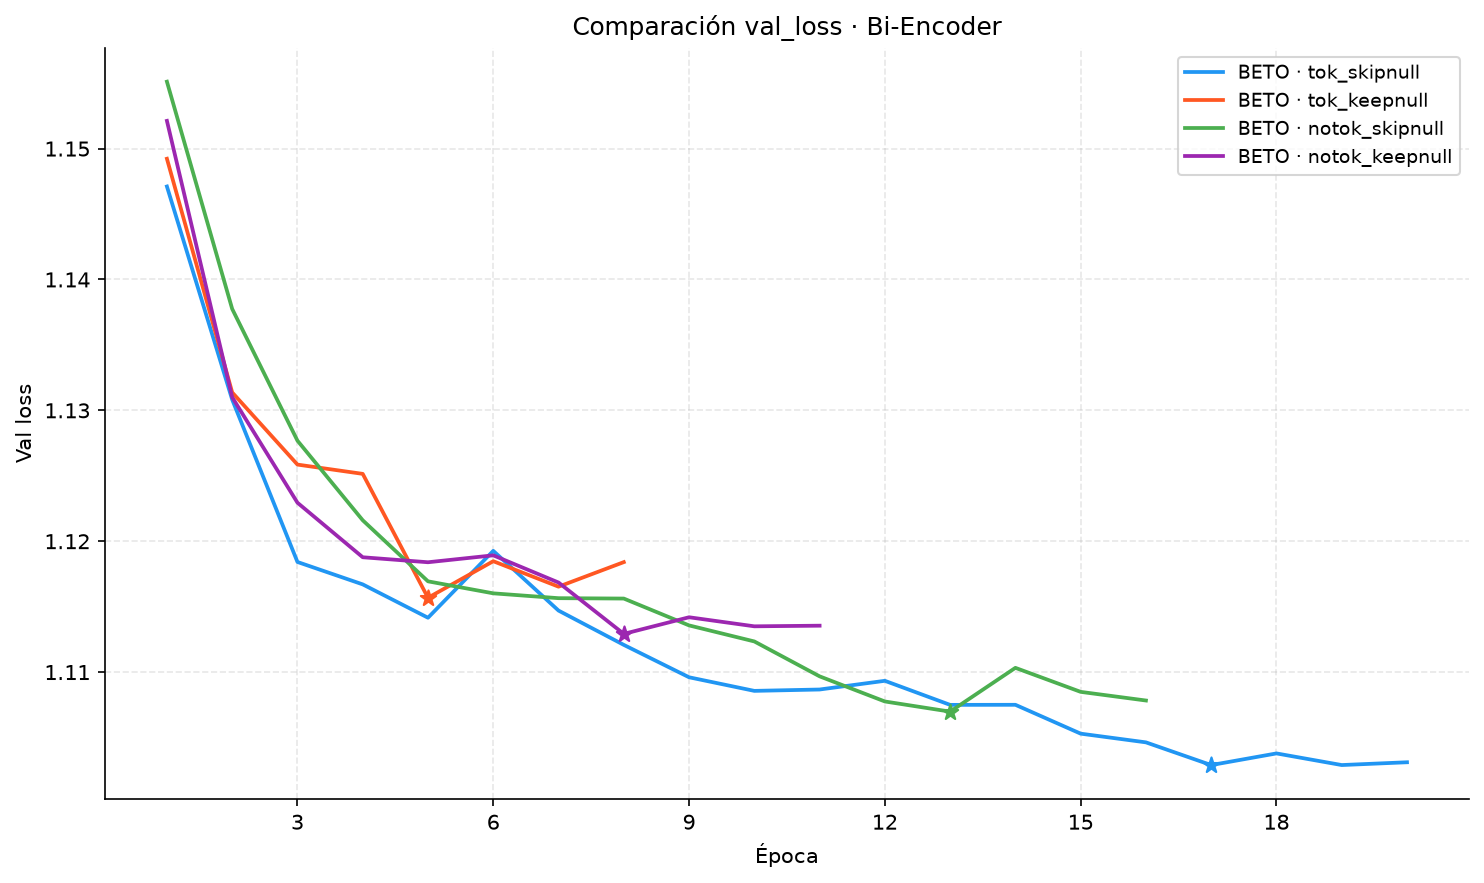
\includegraphics[width=0.90\textwidth]{Figuras/biencoder_serialization_comparison.png}
    \caption{Pérdida de validación por época para las cuatro variantes de serialización del Bi-Encoder BETO. Las estrellas indican el checkpoint de menor pérdida de cada corrida.}
    \label{fig:biencoder_serialization_comparison}
\end{figure}

La Figura~\ref{fig:biencoder_serialization_comparison} muestra además una diferencia en la dinámica de optimización. Las dos variantes que omiten nulos conservaron mejoras durante más épocas. La configuración \texttt{tok\_skipnull} alcanzó su mejor checkpoint en la época 17 y ejecutó 20 épocas; \texttt{notok\_skipnull} alcanzó su mínimo en la época 13 y ejecutó 16. En cambio, los mejores checkpoints de \texttt{tok\_keepnull} y \texttt{notok\_keepnull} ocurrieron en las épocas 5 y 8, y las corridas finalizaron por \textit{early stopping} en las épocas 8 y 11, respectivamente, sin recuperar una mejora sostenida de la pérdida de validación.

La omisión de valores nulos evita repetir información ausente que no discrimina entidades y permite que el modelo continúe refinando la representación con las observaciones disponibles. Los tokens estructurales, por su parte, conservan la delimitación entre bloques y pares clave-valor. Esta combinación permite al modelo identificar qué tipo de información representa cada fragmento sin sobrecargar la secuencia con ausencias. La ventaja en separación es moderada frente a \texttt{notok\_skipnull}, por lo que la conclusión debe interpretarse como una selección empírica dentro de este conjunto de datos y no como una regla universal.


% ==============================================================================
% 5.2 RECUPERACIÓN CON BI-ENCODER
% ==============================================================================
\section{Recuperación eficiente: Bi-Encoder}

Como referencia, se evaluaron sin ajuste fino BETO, RoBERTa-biomedical y paraphrase-multilingual sobre la variante \texttt{notok\_skipnull}. La Tabla~\ref{tab:zeroshot_resultados} muestra que ninguno de los modelos preentrenados produce una recuperación útil sin entrenamiento específico para el problema.

\begin{table}[htbp]
    \centering
    \small
    \caption{Promedios direccionales de los baselines zero-shot en test.}
    \label{tab:zeroshot_resultados}
    \begin{tabular}{lrrr}
        \hline
        Modelo & Recall@1 & MRR & $\Delta_{\mathrm{sep}}$ \\
        \hline
        BETO & 0.0051 & 0.0184 & 0.1583 \\
        RoBERTa-biomedical & 0.0045 & 0.0183 & 0.1651 \\
        paraphrase-multilingual & 0.0047 & 0.0248 & 0.1489 \\
        \hline
    \end{tabular}
\end{table}

Tras el entrenamiento contrastivo, el Bi-Encoder BETO con \texttt{tok\_skipnull} alcanza Recall@1 promedio de 0.9837, Recall@5 perfecto y MRR de 0.9998. La diferencia frente a los baselines confirma que la arquitectura preentrenada por sí sola no organiza los registros institucionales por identidad; el ajuste fino con pares cross-source es el componente que construye el espacio métrico útil para recuperación.


% ==============================================================================
% 5.3 HARD NEGATIVE MINING
% ==============================================================================
\section{Hard Negative Mining}

Con la variante canónica se recuperaron los 20 candidatos más similares por registro para construir los pares del Cross-Encoder. El procedimiento generó 8,513 pares positivos y 69,122 negativos difíciles en entrenamiento; 1,851 y 14,415 en validación; y 1,860 y 14,490 en test, respectivamente.

No se observaron positivos difíciles en las tres particiones: todos los pares positivos conocidos aparecieron en los primeros 20 candidatos. Este resultado confirma que el Bi-Encoder conserva la cobertura necesaria para la segunda etapa. Sin embargo, no demuestra cobertura sobre coincidencias ausentes del \textit{silver standard}; esa limitación se retoma en la discusión final.


% ==============================================================================
% 5.4 CLASIFICACIÓN FINA CON CROSS-ENCODER
% ==============================================================================
\section{Clasificación fina: Cross-Encoder}

El Cross-Encoder recibe los pares plausibles recuperados por el Bi-Encoder y decide si ambos registros pertenecen a la misma entidad. A diferencia de la primera etapa, procesa ambos textos conjuntamente y puede contrastar atributos específicos del par antes de emitir una puntuación. Se entrenó con BETO durante tres épocas sobre 8,513 positivos y 69,122 negativos difíciles, usando BCE ponderada con $\texttt{pos\_weight}=8$. La pérdida de validación descendió de 0.00233 en la primera época a $6.51\times10^{-5}$ en la tercera, que se seleccionó como checkpoint final.

La regla de decisión se ajustó de forma independiente al entrenamiento. Con el checkpoint final fijo, se puntuaron los 16,266 pares de validación y se evaluaron 51 umbrales uniformemente espaciados entre cero y uno. El máximo F1 de validación fue 1.0000 con $\tau=0.12$. Este umbral se congeló antes de evaluar el conjunto de prueba, por lo que las cifras de test no intervienen en su selección.

\begin{table}[htbp]
    \centering
    \small
    \caption{Evaluación del Cross-Encoder canónico en test con $\tau=0.12$.}
    \label{tab:cross_encoder_results}
    \begin{tabular}{l r}
        \hline
        Métrica & Valor \\
        \hline
        Pares evaluados & 16,350 \\
        F1 & 0.9997 \\
        Precisión & 1.0000 \\
        Recall & 0.9995 \\
        Exactitud & 0.9999 \\
        PR-AUC / ROC-AUC & 1.0000 / 1.0000 \\
        Verdaderos positivos / negativos & 1,859 / 14,490 \\
        Falsos positivos / negativos & 0 / 1 \\
        \hline
    \end{tabular}
\end{table}

La distribución de puntuaciones confirma la separación lograda en los pares candidatos: la media de los positivos fue 0.99943 (desviación estándar 0.02318), mientras que la de los negativos fue $2.90\times10^{-5}$ (desviación estándar $6.82\times10^{-5}$). Este resultado no implica que la tarea completa esté resuelta, pues mide solo los pares propuestos por la etapa de recuperación y las etiquetas disponibles constituyen un \textit{silver standard}.

La inspección del único falso negativo, correspondiente al caso PRADO APOLINAR, reveló una inconsistencia en el \textit{ground truth}: los registros atribuidos a una misma entidad contenían nombres y eventos incompatibles. El modelo asignó una puntuación de 0.0001 al par. Más que interpretar el caso como una prueba concluyente de exactitud, se considera evidencia de que el modelo puede apoyar la auditoría de etiquetas y priorizar casos para revisión humana. La calibración mediante \textit{temperature scaling} se ejecutó después de esta evaluación para analizar incertidumbre; no volvió a seleccionar ni modificó el umbral de decisión.


% ==============================================================================
% 5.5 VISUALIZACIÓN UMAP
% ==============================================================================
\section{Visualización del espacio métrico}

Para examinar cualitativamente la estructura aprendida por el Bi-Encoder, se proyectaron sus embeddings de 768 dimensiones a tres dimensiones mediante UMAP (\textit{Uniform Manifold Approximation and Projection})~\cite{mcinnes2018}. UMAP construye primero un grafo ponderado de vecindades en el espacio original y después optimiza una representación de baja dimensionalidad que preserva, en lo posible, esas relaciones locales. Esta técnica permite inspeccionar en una misma figura cómo se distribuyen registros de distintas fuentes y si las observaciones de una misma entidad ocupan vecindades comunes; no se utiliza como medida de desempeño ni como sustituto de la evaluación de recuperación.

La Figura~\ref{fig:umap_entidad_471} muestra una vista 3D de los registros pertenecientes a entidades observadas en más de una fuente. Cada punto corresponde a un registro y el color identifica su base de origen. Las anotaciones destacan los tres registros de la entidad 471, correspondientes a JUAN SANCHEZ LAGUNES, provenientes de Económico, Comorbilidad y Trabajo Social. Los tres puntos se encuentran en la misma vecindad local a pesar de las variaciones en el orden del nombre entre fuentes, lo que ilustra el comportamiento que se busca inducir mediante el entrenamiento contrastivo.

\begin{figure}[htbp]
    \centering
    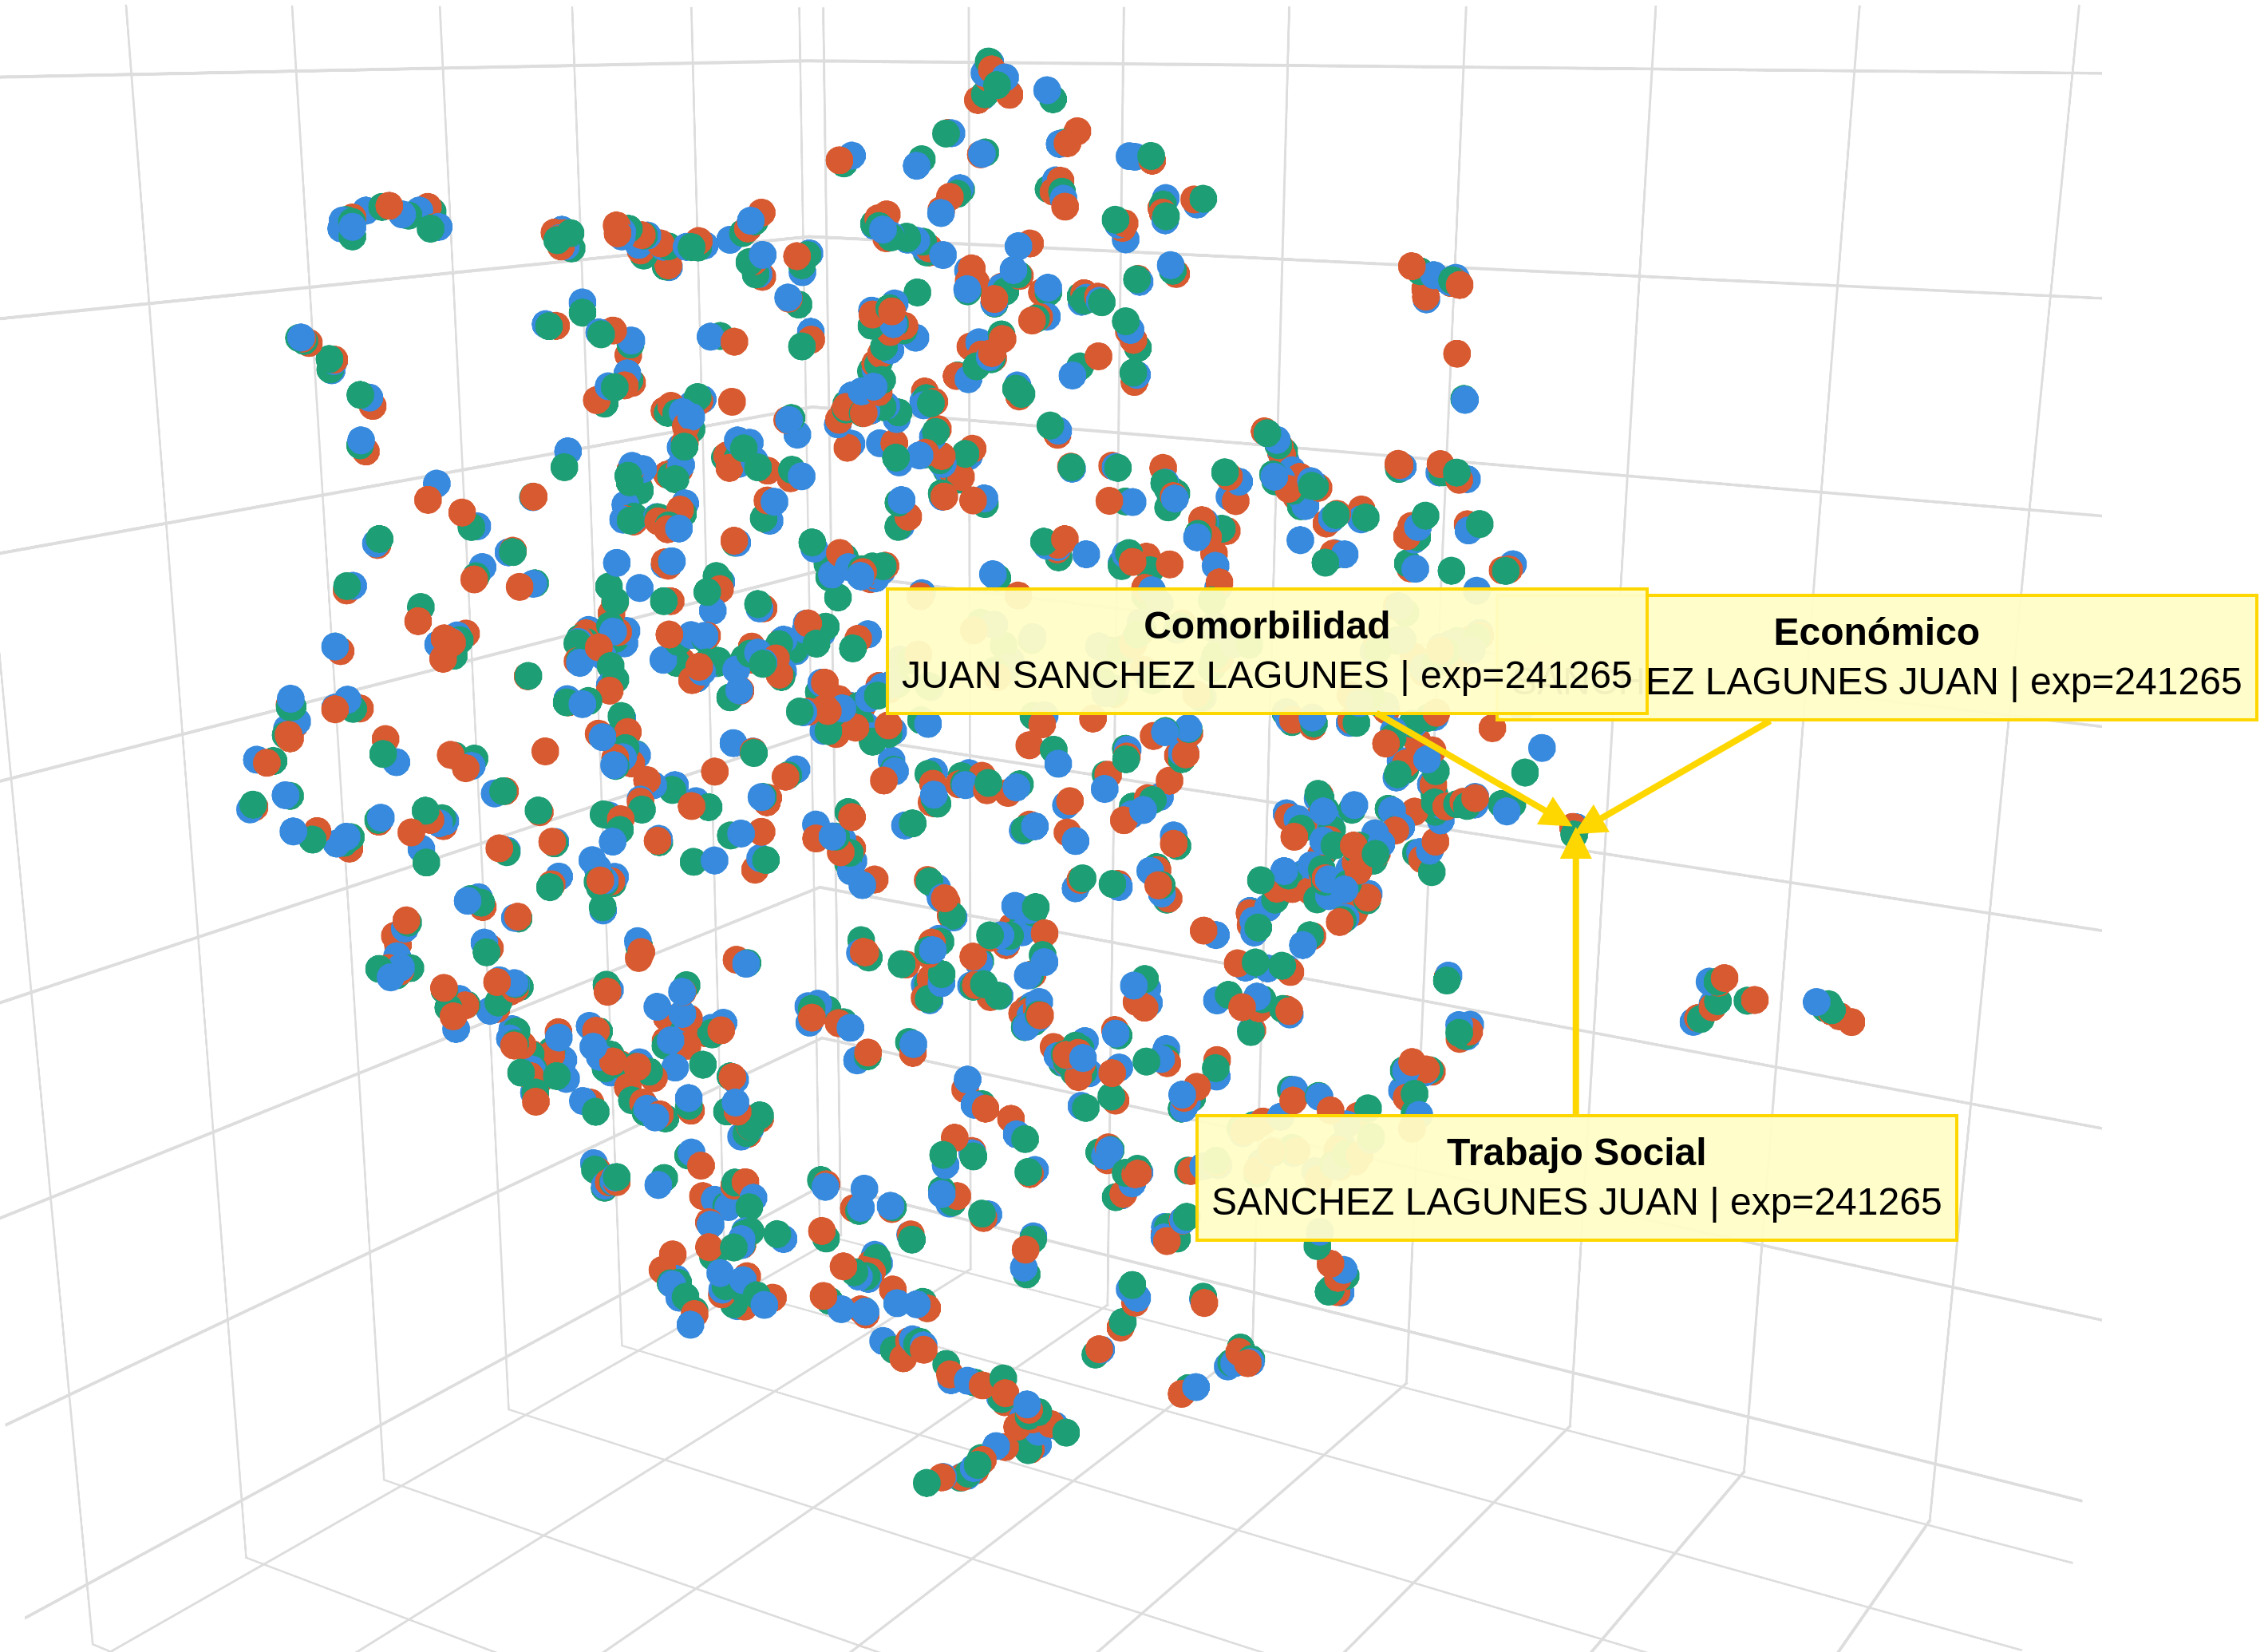
\includegraphics[width=\textwidth]{Figuras/umap_entidad_471_poster.png}
    \caption{Proyección UMAP tridimensional del espacio métrico aprendido por el Bi-Encoder. Cada punto representa un registro de una entidad presente en más de una fuente y el color identifica la base de origen. Las anotaciones resaltan los tres registros de la entidad 471, que quedan ubicados en una misma vecindad local.}
    \label{fig:umap_entidad_471}
\end{figure}

La proximidad visual de esos puntos es consistente con las métricas de recuperación y separación reportadas anteriormente, pero su interpretación debe mantenerse acotada. UMAP privilegia la preservación de estructura local y puede distorsionar distancias globales; por tanto, la figura sirve para comunicar y diagnosticar el espacio aprendido, no para demostrar por sí sola la cobertura de coincidencias no observadas ni la calidad del sistema completo.


% ==============================================================================
% 5.6 CALIBRACIÓN E INCERTIDUMBRE
% ==============================================================================
\section{Calibración e incertidumbre}

La calibración mediante \textit{temperature scaling} se ejecutó después de fijar el umbral y no modificó la regla de decisión. Sobre validación, el ajuste produjo $T=0.065256$, con ECE de $3.7\times10^{-5}$ antes de calibrar y 0 después. La validación perfectamente separable hizo que la transformación llevara las probabilidades calibradas a valores extremos; en test, la entropía calibrada media fue prácticamente nula.

Por esta razón, el diagnóstico de ambigüedad se realizó con la entropía de la puntuación cruda. Nueve de los 16,350 pares de test alcanzaron $H(p)\geq0.01$ bits; ninguno superó 0.1 bits. El Parquet de incertidumbre conserva, por par, la puntuación cruda, la probabilidad calibrada, ambas entropías y el margen respecto de $\tau=0.12$. El caso PRADO ilustra el límite de esta lectura: una predicción muy confiada puede discrepar de una etiqueta que posteriormente requiere revisión. La incertidumbre cuantificada se limita a los pares que llegan al Cross-Encoder; no incorpora posibles coincidencias que la etapa de recuperación no haya propuesto.


% ==============================================================================
% 5.7 DISCUSIÓN INTEGRADORA
% ==============================================================================
\section{Discusión integradora}

El sistema \textit{Retrieve \& Re-rank} logra una recuperación de alta cobertura y una clasificación casi perfecta respecto del \textit{silver standard} disponible. La comparación entre variantes identifica a \texttt{tok\_skipnull} como la mejor configuración dentro del experimento, aunque la ventaja en separación frente a \texttt{notok\_skipnull} es reducida. Esta conclusión se sostiene en pérdida de validación y $\Delta_{\mathrm{sep}}$, pues las métricas de ranking se saturan en el conjunto de prueba.

El resultado no equivale a una validación clínica ni a una garantía de que se recuperen todas las coincidencias reales. Las etiquetas fueron construidas mediante un proceso de consolidación y revisión, por lo que pueden conservar errores o coincidencias no observadas. En consecuencia, el sistema debe entenderse como un apoyo a la integración de registros y a la priorización de revisión humana, no como un sustituto autónomo de validación institucional.


\chapter{Conclusiones}

% ==============================================================================
% 6.1 CONTRIBUCIONES
% ==============================================================================
\section{Resumen de contribuciones}

\textbf{Estructura:}
\begin{itemize}
    \item Se implementó y validó un pipeline completo de Record Linkage neuronal (Retrieve \& Re-rank) sobre bases de datos clínicas reales del INER, alcanzando F1 $\approx$ 1.0 en el silver standard generado.
    \item Contribución metodológica: la serialización \texttt{tok\_skipnull} (tokens de bloque semántico + omisión de nulos) como configuración óptima para Early Fusion en registros tabulares heterogéneos.
    \item Contribución experimental: $\Delta_{\text{sep}}$ como métrica discriminativa para evaluar Bi-Encoders cuando Recall@K se satura.
    \item Contribución práctica: el pipeline de etiquetado determinístico (Ruta A) con revisión manual produjo 11,447 pares confirmados (+1,592 vs baseline), y el Cross-Encoder demostró capacidad de auditoría al detectar un error de etiquetado humano (caso PRADO).
    \item La arquitectura se entrenó y evaluó en HPC con CUDA; el mejor modelo (BETO, MNRL, 17 épocas) y su checkpoint están disponibles para reproducción.
\end{itemize}


% ==============================================================================
% 6.2 LIMITACIONES
% ==============================================================================
\section{Limitaciones}

Los resultados deben interpretarse dentro de los límites del conjunto de datos, del protocolo de evaluación y de la arquitectura implementada.
\begin{itemize}
    \item \textbf{Conjunto de referencia imperfecto:} las etiquetas constituyen un \textit{silver standard}, construido a partir del expediente, reglas determinísticas y revisión manual. Puede contener errores residuales y puede omitir coincidencias reales cuando el expediente difiere entre fuentes.
    \item \textbf{Cobertura condicionada a los candidatos recuperados:} el Cross-Encoder solo evalúa los pares que el Bi-Encoder recupera entre sus candidatos. Dada la naturaleza imperfecta del conjunto de referencia y la ambigüedad de los datos, no puede descartarse que existan coincidencias reales fuera de ese conjunto de candidatos.
    \item \textbf{Entrada limitada del Cross-Encoder:} cada par se procesa en un orden fijo y comparte una ventana máxima de 512 tokens. En una parte de los pares la secuencia excede ese límite y se trunca, por lo que no toda la información de ambos registros llega al clasificador.
    \item \textbf{Incertidumbre acotada:} la calibración y el análisis de incertidumbre se aplicaron a la decisión del Cross-Encoder, no a la etapa de recuperación. La métrica $\Delta_{\mathrm{sep}}$ describe la separación sobre los pares observados del split, pero no cuantifica coincidencias reales que no hayan sido incluidas en el conjunto de referencia.
    \item \textbf{Robustez y generalización:} los operadores de aumento genéricos no reprodujeron las diferencias reales entre las fuentes y no mejoraron la generalización. Los resultados se limitan a las tres bases clínicas del INER; aplicarlos en otra institución requeriría revisar la representación de campos, reentrenar y validar de nuevo el sistema.
\end{itemize}


% ==============================================================================
% 6.3 TRABAJO FUTURO
% ==============================================================================
\section{Trabajo futuro}

Las extensiones siguientes no son necesarias para interpretar los resultados actuales, pero permitirían evaluar con mayor amplitud la robustez y el alcance operativo del sistema.
\begin{itemize}
    \item \textbf{Robustecer la recuperación y la minería de pares difíciles:} ampliar el conjunto de candidatos para incluir registros presentes en una sola fuente, filtrar comparaciones inválidas antes de elegir los candidatos principales y reportar los resultados según la dirección de búsqueda entre bases.
    \item \textbf{Evaluar el efecto del orden y del truncamiento:} procesar cada par en ambas orientaciones, preservando en cada pasada uno de los registros completo, y combinar ambas puntuaciones antes de tomar una decisión.
    \item \textbf{Auditar coincidencias no observadas:} revisar pares no etiquetados con alta similitud y candidatos próximos al límite de recuperación para buscar coincidencias que el conjunto de referencia no contiene.
    \item \textbf{Comparar con una referencia léxica (baseline):} contrastar el enfoque neuronal con representaciones TF-IDF en ambas etapas: recuperación mediante similitud léxica para el Bi-Encoder y clasificación de características del par para el Cross-Encoder. Cada etapa requiere un método apropiado, pero la comparación permitiría aislar la contribución del modelado contextual frente a alternativas clásicas.
    \item \textbf{Estimar la estabilidad del desempeño:} complementar la partición actual con validación cruzada K-fold por entidad. Una evaluación completa exigiría entrenar un nuevo Bi-Encoder en cada partición, regenerar los candidatos y los pares difíciles, y entrenar después un nuevo Cross-Encoder; por ello, multiplica de manera importante el costo de cómputo y el tiempo experimental.
    \item \textbf{Experimento de ablación de bloques semánticos:} retirar un bloque a la vez en el conjunto de prueba y medir el cambio en el desempeño, para identificar qué información contribuye a las decisiones del sistema.
    \item \textbf{Validación y operación en otros contextos:} evaluar el método con datos de otras instituciones e incorporar mecanismos de búsqueda eficientes y herramientas de apoyo a la revisión humana cuando exista un flujo de inferencia definido.
\end{itemize}


% ==============================================================================
% 6.4 CIERRE
% ==============================================================================
\section{Palabras finales}

\textbf{Estructura:}
\begin{itemize}
    \item Párrafo de cierre: la resolución de entidades en bases de datos clínicas fragmentadas es un problema vigente y relevante para la salud pública en México. Este trabajo demostró que un enfoque neuronal basado en aprendizaje métrico y modelos de lenguaje pre-entrenados puede alcanzar precisión de producción, siempre que se acompañe de un proceso cuidadoso de etiquetado y validación humana. La combinación de métodos determinísticos, revisión humana y representaciones semánticas profundas ofrece una ruta viable para integrar sistemas de información hospitalaria heredados sin requerir armonización previa de esquemas.
\end{itemize}


%%%%%%%%%%%%%%%%%%%%%%%%%%%%%%%%%%%%%%%%%%%%%%
%%%           Bibliografía                 %%%
%%%%%%%%%%%%%%%%%%%%%%%%%%%%%%%%%%%%%%%%%%%%%%
\backmatter
\printbibliography

\end{document}
